%=====================================================================
%  BÁO CÁO ĐỒ ÁN TỐT NGHIỆP
%  Đề tài: Xây dựng hệ thống quản lý văn phòng chia sẻ (CoSpace)
%  Trường ĐH Bách khoa - ĐHQG TP.HCM, Khoa KH & KT Máy tính
%---------------------------------------------------------------------
%  Cách biên dịch:  pdflatex main  ->  pdflatex main  ->  pdflatex main
%  (hoặc: latexmk -pdf main.tex)
%---------------------------------------------------------------------
%  Khi nộp bản chính thức: mở preamble.tex, đổi \hienghichutrue
%  thành \hienghichufalse để ẩn toàn bộ khung hướng dẫn màu xám.
%=====================================================================
\documentclass[a4paper,13pt,oneside]{report}
%=====================================================================
%  preamble.tex — Cấu hình chung cho báo cáo Đồ án Tốt nghiệp
%  Biên dịch: pdflatex (chạy 2-3 lần để cập nhật mục lục / tham chiếu)
%=====================================================================

%---------------------- Ngôn ngữ & phông chữ -------------------------
\usepackage[utf8]{vntex}
\usepackage{mathptmx}          % Times New Roman cho cả văn bản và công thức

%---------------------- Trình bày trang ------------------------------
\usepackage{geometry}
\geometry{a4paper, left=30mm, right=20mm, top=25mm, bottom=25mm}
\usepackage{setspace}
\onehalfspacing                % Giãn dòng 1.5 theo quy định báo cáo
\setlength{\parindent}{1cm}
\usepackage{indentfirst}
\usepackage{lastpage}
\usepackage{emptypage}

%---------------------- Bảng biểu & hình ảnh -------------------------
\usepackage{graphicx}
\graphicspath{{Images/}{../Images/}}   % dùng lại kho ảnh của báo cáo ĐACN
\usepackage{array, multirow, multicol, longtable, tabularx, booktabs, hhline}
\usepackage{float}
\usepackage{caption, subcaption}
\usepackage{rotating}
\usepackage{diagbox}
\usepackage{tikz}
\usetikzlibrary{arrows, backgrounds, calc, positioning, shapes.geometric}

%---------------------- Toán học & thuật toán ------------------------
\usepackage{amsmath, amssymb, amsthm}
\usepackage[lined, boxed, commentsnumbered]{algorithm2e}

%---------------------- Mã nguồn -------------------------------------
\usepackage{xcolor}
\usepackage{listings}
\lstdefinestyle{cospace}{
    basicstyle=\footnotesize\ttfamily,
    keywordstyle=\color{blue!70!black}\bfseries,
    commentstyle=\color{green!40!black}\itshape,
    stringstyle=\color{red!60!black},
    numbers=left, numberstyle=\tiny\color{gray}, numbersep=8pt,
    frame=single, rulecolor=\color{gray!50},
    backgroundcolor=\color{gray!5},
    breaklines=true, breakatwhitespace=false,
    showstringspaces=false, tabsize=2, captionpos=b,
    extendedchars=true, literate={ă}{{\u a}}1 {â}{{\^a}}1 {đ}{{\dj}}1 {ê}{{\^e}}1 {ô}{{\^o}}1 {ơ}{{\ohorn}}1 {ư}{{\uhorn}}1
}
\lstset{style=cospace}

%---------------------- Danh mục & liên kết --------------------------
\usepackage[unicode]{hyperref}
\hypersetup{
    colorlinks=true,
    linkcolor=black, citecolor=black, urlcolor=blue,
    pdftitle={Bao cao Do an Tot nghiep - He thong quan ly Co-working Space CoSpace},
    pdfauthor={Vuong Song Toan - Le Dang Khoa}
}
\usepackage[nottoc]{tocbibind}   % đưa Tài liệu tham khảo vào mục lục

%---------------------- Việt hóa tên mục ----------------------------
\renewcommand{\chaptername}{Chương}
\renewcommand{\contentsname}{Mục lục}
\renewcommand{\listfigurename}{Danh sách hình vẽ}
\renewcommand{\listtablename}{Danh sách bảng}
\renewcommand{\bibname}{Tài liệu tham khảo}
\renewcommand{\appendixname}{Phụ lục}
\renewcommand{\figurename}{Hình}
\renewcommand{\tablename}{Bảng}
\renewcommand{\lstlistingname}{Đoạn mã}

%---------------------- Đầu trang / chân trang -----------------------
\usepackage{fancyhdr}
\setlength{\headheight}{40pt}
\pagestyle{fancy}
\fancyhf{}
\fancyhead[L]{%
 \begin{tabular}{rl}
    \begin{picture}(25,15)(0,0)
    \put(0,-8){
\includegraphics[width=10mm, height=10mm]{hcmut.png}}
   \end{picture}&
	\begin{tabular}{l}
		\textbf{\small Trường Đại học Bách khoa -- Đại học Quốc gia TP.HCM}\
		\textbf{\small Khoa Khoa học \& Kỹ thuật Máy tính}
	\end{tabular}
 \end{tabular}%
}
\fancyfoot[L]{\scriptsize Báo cáo Đồ án Tốt nghiệp -- Hệ thống quản lý văn phòng chia sẻ CoSpace}
\fancyfoot[R]{\scriptsize Trang {\thepage}/\pageref{LastPage}}
\renewcommand{\headrulewidth}{0.3pt}
\renewcommand{\footrulewidth}{0.3pt}
\fancypagestyle{plain}{%   % trang đầu mỗi chương vẫn giữ header/footer
  \fancyhf{}
  \fancyhead[L]{%
    \begin{tabular}{rl}
      \begin{picture}(25,15)(0,0)\put(0,-8){
\includegraphics[width=10mm, height=10mm]{hcmut.png}}\end{picture}&
      \begin{tabular}{l}
        \textbf{\small Trường Đại học Bách khoa -- Đại học Quốc gia TP.HCM}\
        \textbf{\small Khoa Khoa học \& Kỹ thuật Máy tính}
      \end{tabular}
    \end{tabular}%
  }
  \fancyfoot[L]{\scriptsize Báo cáo Đồ án Tốt nghiệp -- Hệ thống quản lý văn phòng chia sẻ CoSpace}
  \fancyfoot[R]{\scriptsize Trang {\thepage}/\pageref{LastPage}}
}

%---------------------- Cấp mục & đánh số ---------------------------
\setcounter{secnumdepth}{4}
\setcounter{tocdepth}{3}
\makeatletter
\newcounter{subsubsubsection}[subsubsection]
\renewcommand\thesubsubsubsection{\thesubsubsection.\@alph\c@subsubsubsection}
\newcommand\subsubsubsection{\@startsection{subsubsubsection}{4}{\z@}%
    {-3.25ex\@plus -1ex \@minus -.2ex}{1.5ex \@plus .2ex}{\normalfont\normalsize\bfseries}}
\newcommand*\l@subsubsubsection{\@dottedtocline{4}{10.0em}{4.1em}}
\providecommand*{\toclevel@subsubsubsection}{4}
\newcommand*{\subsubsubsectionmark}[1]{}
\makeatother

%---------------------- Định lý / định nghĩa -------------------------
\newtheorem{definition}{\bf Định nghĩa}[chapter]
\newtheorem{theorem}{\bf Định lý}[chapter]
\newtheorem{property}{\bf Tính chất}[chapter]

%=====================================================================
%  CÁC LỆNH TIỆN ÍCH DÙNG TRONG SƯỜN BÁO CÁO
%=====================================================================

% Bật/tắt toàn bộ khung hướng dẫn viết bài:
%   \hienghichutrue  -> hiển thị (khi đang viết nháp)
%   \hienghichufalse -> ẩn hết (khi nộp bản chính thức)
\newif\ifhienghichu
\hienghichutrue

% \ghichu{...} : khung gợi ý nội dung cần viết cho mục đang soạn
\newcommand{\ghichu}[1]{%
  \ifhienghichu
    \par\vspace{2pt}
    \noindent\begin{tikzpicture}
      \node[draw=gray!55, fill=gray!8, rounded corners=3pt, line width=0.4pt,
            inner sep=7pt, text width=\dimexpr\linewidth-18pt\relax, align=justify]
        {\small\itshape\color{black!72}\textbf{[Nội dung cần viết]}~#1};
    \end{tikzpicture}
    \par\vspace{4pt}
  \fi
}

% \nguon{...} : chỉ ra tài liệu/mã nguồn trong repo dùng làm dữ liệu viết mục này
\newcommand{\nguon}[1]{%
  \ifhienghichu
    \par\noindent{\footnotesize\color{blue!45!black}\textbf{Nguồn dữ liệu:} \texttt{#1}}\par\vspace{4pt}
  \fi
}

% \hinhcho{tỉ lệ bề rộng}{chú thích}{nhãn} : chỗ trống chờ chèn hình
\newcommand{\hinhcho}[3]{%
  \begin{figure}[H]
    \centering
    \begin{tikzpicture}
      \node[draw=gray!60, dashed, fill=gray!5, rounded corners=4pt,
            minimum height=3.2cm, text width=\dimexpr#1\linewidth-20pt\relax, align=center]
        {\small\color{black!60}\textit{[Chèn hình: #2]}};
    \end{tikzpicture}
    \caption{#2}
    \label{#3}
  \end{figure}%
}

% \bangcho{chú thích}{nhãn} : chỗ trống chờ chèn bảng
\newcommand{\bangcho}[2]{%
  \begin{table}[H]
    \centering
    \begin{tabular}{|p{0.9\linewidth}|}
      \hline
      \rule{0pt}{2.2cm}\centering\small\color{black!60}\textit{[Chèn bảng: #1]}\tabularnewline
      \hline
    \end{tabular}
    \caption{#1}
    \label{#2}
  \end{table}%
}


%---------------------------------------------------------------------
%  THÔNG TIN ĐỀ TÀI - chỉnh sửa tập trung tại đây
%---------------------------------------------------------------------
\newcommand{\tendetai}{XÂY DỰNG HỆ THỐNG QUẢN LÝ VĂN PHÒNG CHIA SẺ}
\newcommand{\tendetaiphu}{(CoSpace -- Co-working Space Management System)}
\newcommand{\nganh}{KHOA HỌC MÁY TÍNH}
\newcommand{\hoidong}{\ldots\ldots\ldots}          % TODO: điền hội đồng
\newcommand{\gvhd}{ThS. Trương Quỳnh Chi}
\newcommand{\gvpb}{\ldots\ldots\ldots}             % TODO: điền GV phản biện
\newcommand{\svmot}{Vương Song Toàn (2213544)}
\newcommand{\svhai}{Lê Đăng Khoa (2211599)}
\newcommand{\thoigian}{TP. HỒ CHÍ MINH, THÁNG 12/NĂM 2026}  % TODO: chỉnh tháng bảo vệ

\begin{document}
\hypersetup{pageanchor=false}

%=====================================================================
%  TRANG BÌA
%=====================================================================
\begin{titlepage}
\begin{tikzpicture}[remember picture, overlay]
  \draw[line width=4pt] ($(current page.north west)+(0.4in,-0.5in)$) rectangle ($(current page.south east)+(-0.4in,0.5in)$);
  \draw[line width=1.5pt] ($(current page.north west)+(0.45in,-0.55in)$) rectangle ($(current page.south east)+(-0.45in,0.55in)$);
\end{tikzpicture}

\begin{center}
\LARGE \textbf{ĐẠI HỌC QUỐC GIA THÀNH PHỐ HỒ CHÍ MINH}\\[0.2cm]
\LARGE \textbf{TRƯỜNG ĐẠI HỌC BÁCH KHOA}\\[0.2cm]
\LARGE \textbf{KHOA KHOA HỌC VÀ KỸ THUẬT MÁY TÍNH}
\end{center}

\vspace{0.4cm}
\begin{figure}[h!]
\centering

\includegraphics[width=4cm]{hcmut.png}
\end{figure}

\begin{center}
\parbox{0.95\textwidth}{\centering
\textbf{{\LARGE BÁO CÁO}}\\[0.25cm]
\textbf{{\LARGE ĐỒ ÁN TỐT NGHIỆP}}\\[0.6cm]
\textbf{\LARGE ĐỀ TÀI:}\\[0.2cm]
\textbf{\LARGE \tendetai}\\[0.25cm]
{\large \tendetaiphu}\\[0.6cm]
{\Large NGÀNH: \nganh}
}
\end{center}

\vspace{0.6cm}
\begin{table}[h]
\begin{tabular}{rll}
\hspace{4.5cm} & \textbf{\Large HỘI ĐỒNG:} & {\Large \hoidong}\\[0.35cm]
\hspace{4.5cm} & \textbf{\Large GVHD:}     & {\Large \gvhd}\\[0.35cm]
\hspace{4.5cm} & \textbf{\Large GVPB:}     & {\Large \gvpb}\\[0.35cm]
\hspace{4.5cm} & \multicolumn{2}{l}{\hspace{2.2cm}\textbf{\Large ---o0o---}}\\[0.35cm]
\hspace{4.5cm} & \textbf{\Large SVTH 1:}   & {\Large \svmot}\\[0.35cm]
\hspace{4.5cm} & \textbf{\Large SVTH 2:}   & {\Large \svhai}\\[0.35cm]
\end{tabular}
\end{table}

\vspace{0.4cm}
\begin{center}{\Large \thoigian}\end{center}
\end{titlepage}

%=====================================================================
%  PHẦN ĐẦU (đánh số La Mã)
%=====================================================================
\pagenumbering{roman}
\chapter*{Lời cảm ơn}
\addcontentsline{toc}{chapter}{Lời cảm ơn}
\markboth{LỜI CẢM ƠN}{}

Đồ án Tốt nghiệp là dấu mốc quan trọng khép lại chặng đường học tập, rèn luyện và nghiên cứu của chúng em dưới mái trường Đại học Bách Khoa -- Đại học Quốc gia Thành phố Hồ Chí Minh. Để hoàn thành được công trình nghiên cứu và phát triển phần mềm này, chúng em đã nhận được sự dạy dỗ tận tâm, hỗ trợ chuyên môn sâu sắc và động viên to lớn từ quý Thầy Cô, gia đình và bạn bè.

Lời đầu tiên, chúng em xin bày tỏ lòng biết ơn sâu sắc và chân thành nhất đến \textbf{ThS. Trương Quỳnh Chi}, người cán bộ hướng dẫn đã tận tụy đồng hành, định hướng nghiên cứu và góp ý chuyên môn quý báu cho chúng em trong suốt quá trình thực hiện đồ án. Những nhận xét sắc bén, những định hướng kiến trúc chuẩn mực và sự chỉ bảo tỉ mỉ của Cô không chỉ giúp hệ thống CoSpace đạt được sự hoàn thiện về mặt kỹ thuật mà còn giúp chúng em rèn luyện tác phong nghiên cứu khoa học, kỷ luật công nghệ và tinh thần trách nhiệm của người kỹ sư công nghệ thông tin.

Chúng em cũng xin trân trọng gửi lời tri ân đến Ban Giám hiệu Trường Đại học Bách Khoa cùng toàn thể quý Thầy Cô Khoa Khoa học và Kỹ thuật Máy tính. Những nền tảng kiến thức vững chắc, tư duy hệ thống và phương pháp luận kỹ thuật mà quý Thầy Cô đã truyền đạt trong suốt bốn năm học vừa qua chính là hành trang cốt lõi giúp chúng em tự tin tiếp cận, phân tích và giải quyết trọn vẹn bài toán thực tế của đề tài này. Chúng em xin chân thành cảm ơn quý Thầy Cô trong Hội đồng phản biện và chấm đồ án đã dành thời gian quý báu để đọc, đánh giá và đóng góp các nhận xét chuyên môn nhằm giúp công trình của chúng em được hoàn thiện hơn nữa.

Cuối cùng, chúng con xin gửi lời cảm ơn và lòng tri ân sâu sắc nhất tới cha mẹ và gia đình, những người luôn là điểm tựa tinh thần vững chắc, thầm lặng hy sinh, ủng hộ và tiếp thêm niềm tin cho chúng con trên mọi chặng đường học tập. Nhóm cũng xin gửi lời cảm ơn đến tất cả bạn bè, đồng môn đã luôn đồng hành, thảo luận và hỗ trợ lẫn nhau trong suốt những năm tháng đại học.

Mặc dù nhóm đã nỗ lực hết mình với tinh thần nghiêm túc và cầu thị cao nhất, song do giới hạn về thời gian và kinh nghiệm thực tiễn, báo cáo khó tránh khỏi những điểm còn thiếu sót. Chúng em rất mong nhận được những nhận xét, góp ý và chỉ dẫn quý báu từ quý Thầy Cô và các bạn.

\vspace{1.5cm}
\begin{flushright}
\textit{TP. Hồ Chí Minh, tháng 12 năm 2026}\\[0.4cm]
\textbf{Nhóm sinh viên thực hiện}\\[1.5cm]
\textbf{Vương Song Toàn \hspace{1.5cm} Lê Đăng Khoa}
\end{flushright}

\chapter*{Lời cam đoan}
\addcontentsline{toc}{chapter}{Lời cam đoan}
\markboth{LỜI CAM ĐOAN}{}

\ghichu{Cam đoan đề tài do nhóm tự thực hiện dưới sự hướng dẫn của giảng viên; các số liệu, kết quả kiểm thử và hình ảnh trong báo cáo là trung thực, thu được từ hệ thống do nhóm xây dựng; mọi tài liệu tham khảo đều được trích dẫn đầy đủ trong mục Tài liệu tham khảo. Nêu rõ phần nào sử dụng thư viện/dịch vụ bên thứ ba (Supabase, PayOS, MoMo, Google Gemini) và phạm vi sử dụng.}
\nguon{report/Intro/LoiCamDoan.tex}

\vspace{2cm}
\begin{flushright}
\textbf{Nhóm sinh viên thực hiện}
\end{flushright}

\chapter*{Tóm tắt đề tài}
\addcontentsline{toc}{chapter}{Tóm tắt đề tài}
\markboth{TÓM TẮT ĐỀ TÀI}{}

\ghichu{Viết 3--5 đoạn (khoảng 1 trang) theo mạch: (1) Bối cảnh và vấn đề của mô hình văn phòng chia sẻ đa chi nhánh; (2) Đề tài giải quyết gì --- nền tảng quản lý tập trung gồm quản lý không gian phân cấp, sơ đồ mặt bằng SVG tương tác, đặt chỗ chống xung đột, đa cổng thanh toán, hủy--hoàn tiền tự động, check-in/check-out, kết nối cộng đồng và trợ lý ảo AI; (3) Phương pháp và công nghệ --- Spring Boot 3, React 18/TypeScript, PostgreSQL/Supabase, Docker, triển khai đám mây; (4) Kết quả đạt được, có số liệu cụ thể (số bảng CSDL, số API, số ca kiểm thử, hiệu năng); (5) Hướng phát triển.}
\nguon{docs/SYSTEM_SPEC.md \S1 --- report/Intro/TomTat.tex (bản Đồ án chuyên ngành)}

\vspace{0.6cm}
\noindent\textbf{Từ khóa:} co-working space, đặt chỗ trực tuyến, chống xung đột đồng thời, advisory lock, tích hợp thanh toán, gợi ý đối tác, trợ lý ảo AI.

\ghichu{Nếu hội đồng yêu cầu, bổ sung bản tóm tắt tiếng Anh (Abstract) với nội dung tương đương ngay sau phần này.}

\chapter*{Danh mục từ viết tắt và thuật ngữ}
\addcontentsline{toc}{chapter}{Danh mục từ viết tắt và thuật ngữ}
\markboth{DANH MỤC TỪ VIẾT TẮT}{}

\ghichu{Liệt kê các từ viết tắt và thuật ngữ xuất hiện trong báo cáo, sắp xếp theo bảng chữ cái. Bảng dưới đây đã điền sẵn các mục chắc chắn dùng đến; bổ sung thêm khi viết các chương sau.}
\nguon{docs/glossary.md}

\begin{longtable}{|p{3cm}|p{5cm}|p{6.5cm}|}
\hline
\textbf{Viết tắt} & \textbf{Thuật ngữ đầy đủ} & \textbf{Giải thích} \
\hline
\endfirsthead
\hline
\textbf{Viết tắt} & \textbf{Thuật ngữ đầy đủ} & \textbf{Giải thích} \
\hline
\endhead
API & Application Programming Interface & Giao diện lập trình ứng dụng \ \hline
CSDL & Cơ sở dữ liệu & Nơi lưu trữ dữ liệu có cấu trúc của hệ thống \ \hline
ERD & Entity Relationship Diagram & Sơ đồ quan hệ thực thể \ \hline
JWT & JSON Web Token & Chuẩn token dùng để xác thực người dùng \ \hline
RBAC & Role-Based Access Control & Kiểm soát truy cập theo vai trò \ \hline
REST & Representational State Transfer & Kiểu kiến trúc thiết kế dịch vụ web \ \hline
SPA & Single Page Application & Ứng dụng web một trang \ \hline
SSO & Single Sign-On & Đăng nhập một lần qua nhà cung cấp danh tính \ \hline
SVG & Scalable Vector Graphics & Định dạng ảnh vector dùng vẽ sơ đồ mặt bằng \ \hline
UAT & User Acceptance Testing & Kiểm thử chấp nhận người dùng \ \hline
\ldots & \ldots & \ldots \ \hline
\caption{Danh mục từ viết tắt sử dụng trong báo cáo}
\label{tab:viettat}
\end{longtable}


\newpage \tableofcontents
\newpage \listoffigures
\newpage \listoftables

%=====================================================================
%  PHẦN NỘI DUNG (đánh số Ả Rập)
%=====================================================================
\newpage
\hypersetup{pageanchor=true}
\pagenumbering{arabic}

\chapter{Giới thiệu đề tài}
\label{ch:gioithieu}

\section{Bối cảnh và động lực thực hiện}
\label{sec:boicanh}

\subsection{Sự phát triển của mô hình văn phòng chia sẻ}
Trong bối cảnh nền kinh tế số và làn sóng khởi nghiệp đổi mới sáng tạo đang phát triển mạnh mẽ tại Việt Nam, nhu cầu về một môi trường làm việc linh hoạt, hiện đại và tối ưu hóa chi phí ngày càng trở nên cấp thiết. Theo các báo cáo nghiên cứu thị trường bất động sản thương mại của CBRE và Savills \cite{fielding2000rest}, thị trường không gian làm việc chia sẻ (Co-working Space) tại các đô thị lớn như TP. Hồ Chí Minh và Hà Nội ghi nhận mức tăng trưởng bình quân trên 20\% mỗi năm trong giai đoạn hậu đại dịch. Sự dịch chuyển từ mô hình văn phòng truyền thống dài hạn sang không gian làm việc linh hoạt (Flexible Workspace) đã trở thành xu thế tất yếu của lực lượng lao động tri thức mới, bao gồm các lập trình viên làm việc tự do (Freelancers), các nhóm làm việc từ xa (Remote teams) và các doanh nghiệp vừa và nhỏ (SMEs).

Mô hình văn phòng chia sẻ mang lại khả năng tối ưu hóa chi phí vận hành đáng kể khi người thuê không phải chịu gánh nặng chi phí đầu tư ban đầu về thiết kế mặt bằng, trang thiết bị văn phòng, mạng Internet hay dịch vụ lễ tân. Thay vì ký kết các hợp đồng thuê mặt bằng cố định kéo dài nhiều năm kèm khoản tiền đặt cọc lớn, doanh nghiệp và cá nhân có thể lựa chọn các gói thuê linh hoạt theo giờ, theo ngày, theo tuần hoặc theo tháng tùy theo nhu cầu sử dụng thực tế.

\subsection{Thực trạng vận hành của các chuỗi văn phòng chia sẻ đa chi nhánh}
Mặc dù nhu cầu thị trường rất lớn, phần lớn các đơn vị kinh doanh văn phòng chia sẻ tại Việt Nam hiện nay, đặc biệt là các chuỗi quy mô vừa và nhỏ (từ 2 đến 10 chi nhánh), vẫn đang vận hành dựa trên các phương thức bán thủ công hoặc chắp vá nhiều công cụ rời rạc. Qua khảo sát thực tế, các khó khăn vận hành điển hình bao gồm:
\begin{itemize}
    \item \textbf{Quản lý chỗ ngồi thủ công và thiếu sơ đồ trực quan:} Thông tin chỗ ngồi thường được theo dõi qua bảng tính (Excel/Google Sheets) hoặc ghi chép sổ sách. Khách hàng không thể nắm bắt được sơ đồ mặt bằng vật lý trực quan, vị trí không gian làm việc thực tế, khoảng cách đến các tiện ích (máy in, quầy cà phê, phòng họp) trước khi đến cơ sở.
    \item \textbf{Xung đột lịch đặt chỗ (Double Booking):} Vào các khung giờ cao điểm, việc nhận đặt chỗ qua nhiều kênh không đồng bộ (tin nhắn Zalo, Fanpage, điện thoại và khách đến trực tiếp tại quầy) thường xuyên dẫn đến tình trạng hai khách hàng cùng đặt một vị trí trong cùng một khoảng thời gian, gây ảnh hưởng nghiêm trọng đến uy tín của thương hiệu.
    \item \textbf{Đối soát thanh toán và quy trình hoàn tiền thủ công:} Việc thanh toán chủ yếu thông qua chuyển khoản ngân hàng truyền thống đòi hỏi nhân viên lễ tân phải đối soát sao kê ngân hàng thủ công, chụp ảnh màn hình và đối chiếu vào cuối ca làm việc. Khi khách hàng có nhu cầu hủy đơn, việc tính toán tiền phạt và hoàn tiền diễn ra chậm trễ, dễ xảy ra sai sót và nhầm lẫn dòng tiền.
    \item \textbf{Chính sách hủy không nhất quán giữa các chi nhánh:} Mỗi chi nhánh tại các vị trí địa lý khác nhau có đặc thù vận hành và chi phí mặt bằng khác nhau, dẫn đến nhu cầu áp dụng biểu phí phạt hủy linh hoạt theo từng chi nhánh. Các công cụ quản lý thủ công hiện tại không thể hỗ trợ phân cấp chính sách theo bậc thời gian một cách tự động và minh bạch.
    \item \textbf{Báo cáo kinh doanh phân mảnh:} Ban giám đốc và các nhà quản lý chi nhánh gặp nhiều khó khăn trong việc tổng hợp số liệu doanh thu thực tế, tính toán tỷ lệ lấp đầy (Occupancy Rate) theo thời gian thực để đưa ra các quyết định điều chỉnh giá hoặc tối ưu hóa diện tích mặt bằng kịp thời.
\end{itemize}

\subsection{Nhu cầu kết nối cộng đồng trong không gian làm việc chung}
Điểm khác biệt cốt lõi tạo nên giá trị gia tăng của mô hình văn phòng chia sẻ so với văn phòng truyền thống chính là \textbf{tính cộng đồng (Community Networking)}. Các thành viên cùng làm việc dưới một mái nhà chung sở hữu những kỹ năng chuyên môn, lĩnh vực hoạt động và nhu cầu tìm kiếm đối tác đa dạng. Tuy nhiên, các hệ thống phần mềm quản lý hiện có trên thị trường hầu như chỉ tập trung vào nghiệp vụ cho thuê mặt bằng vật lý đơn thuần, hoàn toàn bỏ ngỏ bài toán kết nối các thành viên.

Thực tế cho thấy việc giao lưu giữa các cá nhân chủ yếu diễn ra một cách tự phát hoặc thông qua các sự kiện sinh hoạt cộng đồng do ban quản lý tổ chức định kỳ. Nhu cầu xây dựng một nền tảng hỗ trợ thành viên chia sẻ hồ sơ năng lực (Profile), tìm kiếm cộng sự tiềm năng thông qua giải thuật so khớp độ tương đồng và trao đổi thông tin chuyên môn trên bảng tin nội bộ là một động lực then chốt để phát triển hệ thống CoSpace.

\section{Phát biểu bài toán}
\label{sec:baitoan}

Từ những đòi hỏi thực tiễn nêu trên, bài toán đặt ra cho đề tài là: \textbf{Nghiên cứu, thiết kế và xây dựng một hệ thống phần mềm quản lý văn phòng chia sẻ tập trung (CoSpace)}, phục vụ đồng thời bốn nhóm tác nhân gồm: Khách hàng (Customer), Nhân viên vận hành quầy (Staff), Quản lý chi nhánh (Branch Admin) và Quản trị viên hệ thống (Super Admin). 

Hệ thống phải số hóa toàn diện quy trình nghiệp vụ đặt chỗ từ khâu tra cứu trên sơ đồ mặt bằng SVG tương tác, thanh toán trực tuyến qua cổng thanh toán quốc gia VietQR Napas 24/7 và ví điện tử, quản lý nhận và trả phòng (Check-in/Check-out), tự động hóa chính sách hủy--hoàn tiền theo bậc thời gian, đến hỗ trợ kết nối mạng lưới cộng đồng thành viên và trợ lý ảo thông minh. Về mặt kỹ thuật, hệ thống phải giải quyết triệt để bài toán kiểm soát tương tranh dữ liệu tài nguyên hữu hạn (ngăn chặn hoàn toàn việc đặt trùng lịch khi nhiều người cùng thao tác), bảo đảm tính bất biến khi tiếp nhận webhook thanh toán, phân quyền bảo mật chặt chẽ theo vai trò (RBAC) và cô lập dữ liệu tuyệt đối giữa các chi nhánh.

Bảng \ref{tab:vande_chucnang} tổng hợp mối liên kết giữa các vấn đề tồn tại trong thực tiễn vận hành và các giải pháp chức năng tương ứng được đề xuất trong hệ thống CoSpace.

\begin{table}[H]
\centering
\caption{Ánh xạ từ vấn đề thực tiễn sang nhu cầu chức năng của hệ thống CoSpace}
\label{tab:vande_chucnang}
\small
\renewcommand{\arraystretch}{1.25}
\begin{tabular}{|p{4.2cm}|p{5.2cm}|p{5.0cm}|}
\hline
\textbf{Vấn đề thực tiễn} & \textbf{Nhu cầu chức năng hệ thống} & \textbf{Giải pháp kỹ thuật CoSpace} \\
\hline
Khách không hình dung được vị trí chỗ ngồi thực tế & Sơ đồ mặt bằng tương tác theo thời gian thực & Kết xuất đồ họa vector SVG động, tích hợp bộ chọn không gian trực quan \\
\hline
Xung đột trùng lịch khi đặt chỗ đồng thời & Kiểm soát lịch khả dụng, chống đặt trùng lịch tuyệt đối & Khóa tư vấn \texttt{pg\_advisory\_xact\_lock} kết hợp ràng buộc \texttt{EXCLUDE USING gist} \\
\hline
Đối soát thanh toán thủ công, chuyển khoản chậm & Thanh toán tự động, tức thời qua mã QR ngân hàng và ví điện tử & Tích hợp cổng PayOS (chuẩn VietQR) và MoMo; xử lý Webhook bất biến (Idempotency) \\
\hline
Chính sách hủy đơn và hoàn tiền nhập nhằng, chậm trễ & Tự động tính toán mức phạt và hoàn tiền theo bậc thời gian & Thuật toán đối chiếu chính sách chi nhánh/toàn cục; hàng chờ duyệt hoàn tiền minh bạch \\
\hline
Thủ tục check-in tại quầy thủ công, mất thời gian & Check-in một chạm bằng mã định danh đặt chỗ hoặc mã QR & Trình quét mã QR trên nền Web, cửa sổ kiểm tra hợp lệ 30 phút, kiểm soát nợ dịch vụ \\
\hline
Các thành viên không có kênh kết nối hợp tác & Hồ sơ năng lực và gợi ý đối tác tiềm năng tự động & Thuật toán tính độ tương đồng Jaccard kết hợp trọng số kỹ năng và chi nhánh; bảng tin \\
\hline
Quản lý chi nhánh thiếu công cụ điều hành và giá & Phân cấp cấu hình bảng giá, dịch vụ thêm và báo cáo theo chi nhánh & Kiến trúc RBAC kết hợp bảo vệ truy cập tầng chi nhánh (\texttt{BranchAccessGuard}); xuất CSV \\
\hline
\end{tabular}
\end{table}

\section{Mục tiêu đề tài}
\label{sec:muctieu}

\subsection{Mục tiêu về nghiệp vụ}
Đề tài hướng tới việc giải quyết trọn vẹn các bài toán vận hành thông qua các mục tiêu nghiệp vụ cụ thể:
\begin{enumerate}
    \item \textbf{Số hóa toàn diện vòng đời đặt chỗ:} Hỗ trợ khách hàng tìm kiếm, giữ chỗ tạm thời trong 15 phút, thanh toán trực tuyến tức thời và nhận mã QR xác nhận đơn hoàn toàn tự động trên nền tảng web.
    \item \textbf{Quản lý tập trung chuỗi đa chi nhánh:} Cho phép doanh nghiệp mở rộng quy mô nhiều cơ sở, phân tầng quản lý theo Tòa nhà -- Tầng -- Không gian làm việc, hỗ trợ thiết lập bảng giá và dịch vụ gia tăng riêng biệt cho từng chi nhánh.
    \item \textbf{Tự động hóa chính sách hủy và minh bạch hoàn tiền:} Cung cấp cơ chế tính toán phí phạt và số tiền hoàn tự động dựa trên mốc thời gian khách gửi yêu cầu hủy so với thời điểm bắt đầu đơn, giải phóng chỗ trống ngay lập tức cho khách hàng khác.
    \item \textbf{Tối ưu hóa quy trình vận hành quầy:} Trang bị cho nhân viên lễ tân công cụ tạo đơn đặt chỗ tại quầy (Walk-in), thu tiền mặt, thực hiện check-in/check-out một chạm và ghi nhận các dịch vụ gọi thêm vào đơn đang hoạt động.
    \item \textbf{Thúc đẩy gắn kết cộng đồng thành viên:} Cung cấp tính năng xây dựng hồ sơ năng lực cá nhân, thuật toán gợi ý đối tác kinh doanh phù hợp và diễn đàn nội bộ để chia sẻ thông tin, sự kiện và cơ hội hợp tác.
    \item \textbf{Cung cấp hệ thống báo cáo quản trị trực quan:} Giúp ban điều hành nắm bắt doanh thu thực tế, tỷ lệ lấp đầy mặt bằng và so sánh hiệu quả kinh doanh giữa các chi nhánh theo thời gian thực.
\end{enumerate}

\subsection{Mục tiêu về kỹ thuật}
Bên cạnh các yêu cầu nghiệp vụ, đề tài đặt ra các tiêu chuẩn khắt khe về kỹ thuật phần mềm:
\begin{enumerate}
    \item \textbf{Kiến trúc phân tầng và dễ bảo trì:} Xây dựng hệ thống theo mô hình khách--chủ ba tầng (Client--Server 3-Tier), tách bạch rõ ràng giữa tầng trình bày (React/TypeScript), tầng nghiệp vụ (Spring Boot 3) và tầng dữ liệu (PostgreSQL), tuân thủ nguyên lý kiến trúc sạch (Clean Architecture).
    \item \textbf{Bảo đảm tính đúng đắn khi tương tranh cao:} Thiết kế cơ chế khóa hai lớp độc lập ở tầng ứng dụng và tầng cơ sở dữ liệu, cam kết không xảy ra tình trạng đặt trùng lịch (Overbooking) ngay cả khi hàng chục người dùng cùng nhấn nút thanh toán cho cùng một vị trí trong cùng một phần trăm giây.
    \item \textbf{Xử lý Webhook thanh toán an toàn và bất biến:} Xây dựng cơ chế kiểm tra chữ ký điện tử mật mã và chống xử lý trùng lặp giao dịch (Idempotent Consumer), đảm bảo sự kiện thanh toán bị gọi lặp nhiều lần vẫn duy trì kết quả chính xác duy nhất.
    \item \textbf{Bảo mật phân quyền chặt chẽ và cô lập dữ liệu:} Ứng dụng mô hình xác thực kép (Supabase JWT cho đăng nhập mạng xã hội và JWT nội bộ ký HS384), kiểm soát truy cập theo vai trò (RBAC) và cơ chế chốt chặn truy cập chi nhánh ngăn chặn rò rỉ dữ liệu chéo giữa các cơ sở.
    \item \textbf{Tích hợp Trí tuệ nhân tạo có kiểm soát an toàn:} Hiện thực trợ lý ảo thông minh dựa trên mô hình ngôn ngữ lớn (Google Gemini Flash), hỗ trợ cơ chế gọi hàm (Function Calling) với rào chắn bắt buộc khách hàng xác nhận trước khi thực hiện các giao dịch làm thay đổi dữ liệu thật.
    \item \textbf{Khả năng triển khai và vận hành đám mây:} Đóng gói ứng dụng thành các Docker container tinh gọn thông qua kỹ thuật Multi-stage build và tự động hóa quy trình phát hành lên các nền tảng đám mây hiện đại (Vercel, Render và Supabase).
\end{enumerate}

\section{Đối tượng và phạm vi đề tài}
\label{sec:phamvi}

\subsection{Đối tượng người dùng}
Hệ thống CoSpace được thiết kế xoay quanh bốn nhóm tác nhân người dùng với các đặc thù phân quyền và phạm vi dữ liệu rõ ràng:
\begin{itemize}
    \item \textbf{Khách hàng (Customer):} Người thuê không gian làm việc. Khách hàng có thể đăng ký tài khoản tự do, xem sơ đồ mặt bằng, đặt chỗ ngắn hạn (theo giờ/ngày) hoặc dài hạn (theo tuần/tháng), thanh toán trực tuyến, check-in, hủy đơn, tham gia diễn đàn cộng đồng, tìm kiếm đối tác và tương tác với trợ lý ảo. Khách hàng không bị ràng buộc vào một chi nhánh cố định và có thể đặt chỗ tại bất kỳ chi nhánh nào trong hệ thống.
    \item \textbf{Nhân viên vận hành quầy (Staff):} Nhân viên trực ban tại cơ sở. Nhân viên bắt buộc phải gắn với một chi nhánh cụ thể (\texttt{branch\_id}), chỉ có quyền xem và xử lý các đơn đặt chỗ thuộc chi nhánh của mình: tạo đơn tại quầy cho khách vãng lai, thu tiền mặt, thực hiện check-in/out, ghi nhận dịch vụ phát sinh và quản lý lịch bảo trì không gian tại chi nhánh.
    \item \textbf{Quản lý chi nhánh (Branch Admin):} Người chịu trách nhiệm điều hành toàn diện một cơ sở. Quản lý chi nhánh cũng bắt buộc gắn với một \texttt{branch\_id}, có quyền cấu hình không gian làm việc, chỉnh sửa sơ đồ mặt bằng SVG, thiết lập bảng giá riêng, cấu hình biểu phí hủy riêng, quản lý tài khoản nhân viên của cơ sở, duyệt các yêu cầu hoàn tiền và xem báo cáo tài chính nội bộ của chi nhánh.
    \item \textbf{Quản trị viên hệ thống (Super Admin):} Cán bộ quản trị cấp cao nhất của chuỗi. Super Admin không bị giới hạn theo chi nhánh, có quyền tạo mới chi nhánh, quản lý danh mục dùng chung (loại không gian, tiện ích), quản lý toàn bộ tài khoản nhân sự và phân quyền, thiết lập các chính sách toàn cục mặc định, xem báo cáo tổng hợp đối chiếu giữa các cơ sở và tra cứu nhật ký kiểm toán (Audit Log) toàn hệ thống.
\end{itemize}

\subsection{Phạm vi chức năng}
\textbf{Trong phạm vi đề tài (In-scope):}
\begin{itemize}
    \item Quản lý thông tin chuỗi chi nhánh, cấu trúc tòa nhà, tầng và danh mục không gian làm việc phân loại theo đặc tính.
    \item Soạn thảo và hiển thị sơ đồ mặt bằng đồ họa vector tương tác (SVG Floorplan).
    \item Quy trình đặt chỗ ngắn hạn (theo giờ, ngày) và dài hạn (theo tuần, tháng) với cơ chế giữ chỗ tạm thời có thời hạn 15 phút.
    \item Tích hợp cổng thanh toán trực tuyến PayOS (VietQR) và MoMo (Sandbox), cùng phương thức thanh toán tiền mặt tại quầy do nhân viên xác nhận.
    \item Tự động hóa chính sách hủy theo khoảng thời gian và quản lý quy trình duyệt hoàn tiền minh bạch.
    \item Quy trình check-in/out có kiểm tra khung thời gian cho phép (dung sai 30 phút trước giờ bắt đầu) và kiểm tra thanh toán nợ dịch vụ phát sinh.
    \item Quản lý chương trình khuyến mãi (mã giảm giá) và tự động xếp hạng thành viên dựa trên tổng chi tiêu tích lũy.
    \item Quản lý lịch bảo trì cơ sở vật chất và xử lý các đơn đặt chỗ bị ảnh hưởng.
    \item Tính năng mạng lưới cộng đồng: xây dựng hồ sơ năng lực, diễn đàn thảo luận và thuật toán gợi ý đối tác kinh doanh (Smart Matching).
    \item Trợ lý ảo AI đàm thoại tự nhiên, hỗ trợ giải đáp quy chế và thực hiện đặt chỗ thông qua cơ chế Function Calling có xác nhận.
    \item Báo cáo thống kê kinh doanh, tỷ lệ lấp đầy và nhật ký kiểm toán hệ thống.
\end{itemize}

\textbf{Ngoài phạm vi đề tài (Out-of-scope):}
\begin{itemize}
    \item Tính năng tự động giải ngân chi trả tiền hoàn từ tài khoản doanh nghiệp về ví điện tử/tài khoản ngân hàng của khách hàng qua API (hệ thống hiện tại ghi nhận khoản hoàn tiền được duyệt vào sổ cái để quản lý chi nhánh chi trả thủ công).
    \item Ứng dụng di động bản địa (Native Mobile App) trên iOS hoặc Android (hệ thống hiện tập trung tối ưu hóa giao diện Web ứng dụng theo chuẩn Responsive trên thiết bị di động).
    \item Tích hợp trực tiếp với phần cứng kiểm soát ra vào vật lý (khóa cửa từ thông minh, cổng xoay tripod).
    \item Nghiệp vụ kế toán chuyên sâu, quản trị kho hàng chi tiết và quản lý chấm công, tính lương nhân sự.
\end{itemize}

\subsection{Phạm vi triển khai và thử nghiệm}
Hệ thống được phát triển và kiểm thử trên môi trường thử nghiệm với dữ liệu giả lập đại diện cho chuỗi văn phòng gồm 3 chi nhánh tại các khu vực trọng điểm của TP. Hồ Chí Minh. Các cổng thanh toán PayOS và MoMo được vận hành ở chế độ thử nghiệm (Sandbox / Test environment). Toàn bộ hệ thống được triển khai thực tế trên hạ tầng đám mây công cộng (Frontend trên nền tảng Vercel CDN, Backend đóng gói container chạy trên Render và cơ sở dữ liệu PostgreSQL lưu trữ tại Supabase khu vực Châu Á).

\section{Phương pháp thực hiện}
\label{sec:phuongphap}

Đề tài áp dụng quy trình phát triển phần mềm lặp theo mô hình linh hoạt **Agile/Scrum** kết hợp với kỷ luật công nghệ nghiêm ngặt:
\begin{itemize}
    \item \textbf{Phương pháp tiếp cận Document-First \& Database-First:} Trước khi viết mã, toàn bộ các quy tắc nghiệp vụ (48 quy tắc cốt lõi), đặc tả ca sử dụng (Use Cases) và các hợp đồng giao tiếp API (API Contracts) đều được biên soạn và chuẩn hóa dưới dạng tài liệu sống trong thư mục \texttt{docs/}. Lược đồ cơ sở dữ liệu được thiết kế, tối ưu hóa chuẩn 3NF và quản lý phiên bản di trú chặt chẽ bằng Flyway.
    \item \textbf{Phát triển theo vòng lặp gia tăng (Iterative Sprints):} Dự án được chia thành 6 giai đoạn phát triển (Sprints) nối tiếp nhau, mỗi sprint tập trung hoàn thiện trọn vẹn một nhóm tính năng từ Back-end đến Front-end và kiểm thử.
    \item \textbf{Kiểm thử tự động hóa (Automated Testing):} Triển khai kiểm thử đơn vị và kiểm thử lát cắt web (WebMvc Test) ngay trong quá trình viết mã dịch vụ, bảo đảm độ bao phủ các luồng xử lý chính và các nhánh ngoại lệ.
    \item \textbf{Rà soát logic độc lập (Static Logic Audit):} Thực hiện rà soát tĩnh toàn diện mã nguồn xuyên suốt các tầng kiến trúc (Controller $\rightarrow$ Service $\rightarrow$ Repository $\rightarrow$ Database) nhằm phát hiện sớm các nguy cơ tranh chấp tương tranh, sai lệch công thức tài chính và lỗ hổng bảo mật tiềm ẩn.
\end{itemize}

Bảng \ref{tab:kehoach} trình bày kế hoạch thực hiện đề tài qua các tuần và sự phân công trách nhiệm chi tiết giữa hai thành viên trong nhóm.

\begin{table}[H]
\centering
\caption{Kế hoạch thực hiện đề tài theo tuần và phân công công việc}
\label{tab:kehoach}
\small
\renewcommand{\arraystretch}{1.25}
\begin{tabular}{|p{1.6cm}|p{7.2cm}|p{2.6cm}|p{2.6cm}|}
\hline
\textbf{Thời gian} & \textbf{Nội dung công việc} & \textbf{Vương Song Toàn} & \textbf{Lê Đăng Khoa} \\
\hline
Tuần 1--2 & Khảo sát bài toán thực tế, nghiên cứu các hệ thống tương tự, lập tài liệu đặc tả yêu cầu hệ thống (\texttt{SYSTEM\_SPEC.md}) & Phân tích nghiệp vụ, kiến trúc hệ thống & Khảo sát thị trường, yêu cầu chức năng \\
\hline
Tuần 3--4 & Thiết kế lược đồ CSDL quan hệ, thiết kế hợp đồng API RESTful và thiết lập hạ tầng dự án (Spring Boot, React, Supabase) & Thiết kế CSDL, Flyway, cấu hình Security & Dựng khung Front-end, định tuyến và theme \\
\hline
Tuần 5--6 & Hiện thực Module xác thực người dùng (JWT kép, Google SSO), quản lý chi nhánh, tầng và không gian làm việc & Hiện thực dịch vụ Auth, Branch, Space (BE) & Giao diện Đăng nhập, Profile, Quản trị không gian (FE) \\
\hline
Tuần 7--8 & Hiện thực Trình soạn thảo/hiển thị sơ đồ mặt bằng SVG; hiện thực nghiệp vụ Đặt chỗ và 2 tầng khóa tương tranh & Hiện thực dịch vụ Booking, khóa tư vấn (BE) & Trình hiển thị sơ đồ SVG \texttt{FloorPlanViewer} (FE) \\
\hline
Tuần 9--10 & Tích hợp cổng thanh toán VietQR (PayOS), MoMo và cơ chế Webhook bất biến; tự động hóa hết hạn đơn đặt chỗ & Tích hợp PayOS, MoMo, Scheduler hết hạn đơn & Giao diện Checkout, mã QR động, đếm ngược \\
\hline
Tuần 11--12 & Hiện thực quy trình Hủy--Hoàn tiền theo bậc thời gian; Module vận hành Check-in/out và quản lý lịch bảo trì & Dịch vụ Hủy/Hoàn tiền, Check-in, Bảo trì (BE) & Giao diện Quầy Lễ tân, quét mã QR check-in (FE) \\
\hline
Tuần 13--14 & Xây dựng Module gợi ý đối tác (Jaccard) và Trợ lý ảo AI Google Gemini (Function Calling); quản lý khuyến mãi & Dịch vụ Gemini AI, Matching, Loyalty (BE) & Giao diện Cộng đồng, Chatbot Drawer, Thẻ đối tác (FE) \\
\hline
Tuần 15--16 & Báo cáo thống kê doanh thu, tỷ lệ lấp đầy, xuất dữ liệu CSV; nhật ký kiểm toán; tối ưu hóa Docker và triển khai Cloud & Dịch vụ Report, Audit Log, Dockerfile, Render & Giao diện Báo cáo, biểu đồ Recharts, Vercel \\
\hline
Tuần 17--18 & Rà soát logic toàn diện (\texttt{LOGIC\_AUDIT.md}), sửa đổi 55 phát hiện nghiệp vụ, bổ sung kiểm thử tự động & Rà soát BE, sửa lỗi tương tranh, nâng suite test lên 273 ca & Rà soát luồng FE, tối ưu hóa bundle Vite, kiểm thử UAT \\
\hline
Tuần 19--20 & Hoàn thiện báo cáo Đồ án Tốt nghiệp LaTeX, sinh sơ đồ tự động từ mã nguồn, chuẩn bị slide và bảo vệ & Biên soạn Ch06, Ch07, Ch09, Ch10, Phụ lục & Biên soạn Ch01, Ch02, Ch03, Ch04, Ch05, Ch08, Ch11 \\
\hline
\end{tabular}
\end{table}

\section{Ý nghĩa của đề tài}
\label{sec:ynghia}

\subsection{Ý nghĩa khoa học}
Về mặt khoa học máy tính và kỹ thuật phần mềm, đề tài mang lại những giá trị nghiên cứu và thực nghiệm sâu sắc:
\begin{itemize}
    \item \textbf{Vận dụng cơ chế điều khiển tương tranh phân tán ở tầng dữ liệu:} Đề tài cung cấp mô hình thực nghiệm rõ ràng về việc kết hợp giữa khóa tư vấn ở cấp độ giao dịch (\texttt{pg\_advisory\_xact\_lock}) và ràng buộc loại trừ không gian--thời gian (\texttt{EXCLUDE USING gist}) trên PostgreSQL. Mô hình này giải quyết triệt để vấn đề mất tính nhất quán dữ liệu trong bài toán đặt chỗ tài nguyên hữu hạn mà không phải trả giá đắt về hiệu năng hay gây ra hiện tượng khóa chết (Deadlock).
    \item \textbf{Mô hình hóa kiến trúc tích hợp thanh toán bất biến:} Đưa ra giải pháp chuẩn mực trong việc xử lý sự kiện bất đồng bộ từ các bên thứ ba (Webhooks), đảm bảo tính toán vẹn dữ liệu tài chính trong môi trường mạng thiếu tin cậy có độ trễ cao hoặc xảy ra việc gửi lặp sự kiện.
    \item \textbf{Kiểm soát mô hình ngôn ngữ lớn (LLM) trong hệ thống hướng trạng thái:} Vận dụng kỹ thuật Prompt Engineering và Function Calling kết hợp cơ chế kiểm soát giao dịch có rào chắn xác nhận từ người dùng (Confirmation Barrier), mở ra hướng tiếp cận an toàn khi ứng dụng Trí tuệ nhân tạo tạo sinh vào các hệ thống vận hành thực tế.
\end{itemize}

\subsection{Ý nghĩa thực tiễn}
Về mặt ứng dụng kinh tế -- xã hội, đề tài đóng góp một giải pháp công nghệ mang tính ứng dụng cao:
\begin{itemize}
    \item Cung cấp giải pháp chuyển đổi số toàn diện, đóng gói sẵn sàng cho các doanh nghiệp vận hành văn phòng chia sẻ tại Việt Nam, giúp tiết kiệm tới 50\% thời gian bàn giấy của nhân viên lễ tân và loại trừ hoàn toàn các tổn thất doanh thu do lỗi đặt trùng phòng.
    \item Đem lại trải nghiệm dịch vụ tiện nghi, hiện đại và minh bạch cho khách hàng thông qua sơ đồ trực quan và thanh toán không tiền mặt theo đúng chuẩn ngân hàng quốc gia VietQR Napas 24/7.
    \item Xây dựng một không gian mở kết nối cộng đồng tri thức, hỗ trợ các cá nhân làm việc tự do và các nhóm khởi nghiệp tìm kiếm cơ hội hợp tác kinh doanh, đóng góp tích cực vào sự phát triển của hệ sinh thái khởi nghiệp sáng tạo Việt Nam.
\end{itemize}

\section{Cấu trúc báo cáo}
\label{sec:cautruc}

Bản báo cáo Đồ án Tốt nghiệp được tổ chức thành 11 chương nội dung chính cùng các phần phụ lục, trình bày một cách có hệ thống từ khâu khảo sát thực tế, phân tích, thiết kế, hiện thực đến đánh giá nghiệm thu:
\begin{itemize}
    \item \textbf{Chương \ref{ch:gioithieu} -- Giới thiệu đề tài:} Trình bày bối cảnh ra đời, thực trạng vận hành văn phòng chia sẻ, phát biểu bài toán, mục tiêu, đối tượng, phạm vi nghiên cứu và phương pháp thực hiện đề tài.
    \item \textbf{Chương \ref{ch:khaosat} -- Khảo sát và phân tích tổng quan:} Khảo sát chi tiết các mô hình không gian làm việc chung, đánh giá các hệ thống phần mềm trong nước và quốc tế hiện nay, phân tích khoảng trống và đề xuất định vị giải pháp CoSpace cùng các bài toán kỹ thuật trọng tâm.
    \item \textbf{Chương \ref{ch:nentang} -- Kiến thức nền tảng và công nghệ sử dụng:} Cung cấp cơ sở lý thuyết về kiến trúc phân tầng, chuẩn REST, mô hình xác thực OAuth2/JWT, lý thuyết giao dịch tương tranh ACID, độ đo tương đồng Jaccard và mô hình ngôn ngữ lớn LLM; tổng hợp các công nghệ sử dụng phía Client, Server, Database và DevOps.
    \item \textbf{Chương \ref{ch:yeucau} -- Phân tích yêu cầu hệ thống:} Xác định bốn nhóm tác nhân người dùng, đặc tả danh mục yêu cầu chức năng (FR) và phi chức năng (NFR), phân tích hệ thống 48 quy tắc nghiệp vụ cốt lõi, sơ đồ use-case tổng quát và ma trận phân quyền chức năng.
    \item \textbf{Chương \ref{ch:usecase} -- Mô hình hóa và đặc tả use-case:} Chi tiết hóa các use-case của bốn phân hệ, mô hình hóa các quy trình nghiệp vụ cốt lõi bằng sơ đồ hoạt động (Activity Diagrams), diễn giải 14 sơ đồ tuần tự kỹ thuật (Sequence Diagrams) và các mô hình máy trạng thái (Statechart).
    \item \textbf{Chương \ref{ch:thietke} -- Kiến trúc và thiết kế hệ thống:} Trình bày kiến trúc tổng thể ba tầng, thiết kế chi tiết 11 sơ đồ lớp miền dữ liệu và tầng dịch vụ, thiết kế lược đồ cơ sở dữ liệu quan hệ (ERD 30 bảng), thiết kế API và kiến trúc an ninh bảo mật nhiều lớp.
    \item \textbf{Chương \ref{ch:hienthuc} -- Hiện thực hệ thống:} Thuyết minh chi tiết các kỹ thuật lập trình then chốt ở phía máy chủ Spring Boot (khóa tư vấn, xử lý webhook bất biến, bộ lập lịch nền, trợ lý ảo AI) và phía giao diện React/TypeScript (trình kết xuất sơ đồ SVG, đồng hồ đếm ngược, định tuyến bảo vệ).
    \item \textbf{Chương \ref{ch:giaodien} -- Giao diện và kết quả đạt được:} Trình bày hình ảnh và trải nghiệm người dùng thực tế của 33 trang giao diện qua bốn phân hệ, đánh giá khả năng đáp ứng trên các loại thiết bị và đối chiếu mức độ hoàn thành với tập yêu cầu ban đầu.
    \item \textbf{Chương \ref{ch:kiemthu} -- Kiểm thử và đánh giá:} Báo cáo kết quả kiểm thử tự động 273 ca kiểm thử phía máy chủ, kiểm thử tương tranh CSDL, công bố kết quả đợt rà soát logic độc lập (55 phát hiện) và đánh giá hiệu năng hệ thống.
    \item \textbf{Chương \ref{ch:trienkhai} -- Triển khai và vận hành:} Hướng dẫn đóng gói container bằng Docker Multi-stage, cấu hình triển khai trên đám mây Vercel và Render, quản lý biến môi trường an toàn và cơ chế giữ máy chủ hoạt động liên tục.
    \item \textbf{Chương \ref{ch:ketluan} -- Kết luận và hướng phát triển:} Tổng kết các kết quả đạt được, đóng góp chính của đề tài, thẳng thắn chỉ ra các hạn chế kỹ thuật còn tồn đọng, rút ra bài học kinh nghiệm và vạch ra lộ trình phát triển trong tương lai.
    \item \textbf{Phần Phụ lục:} Cung cấp hướng dẫn cài đặt chạy thử nghiệm hệ thống (Phụ lục \ref{pl:caidat}), danh mục toàn bộ 133 điểm cuối API (Phụ lục \ref{pl:api}) và bảng tổng hợp 16 quyết định nghiệp vụ đã chốt sau đợt rà soát logic (Phụ lục \ref{pl:quyetdinh}).
\end{itemize}

\chapter{Khảo sát và phân tích tổng quan}
\label{ch:khaosat}

\ghichu{Chương này chứng minh đề tài có chỗ đứng: trình bày nền tảng khái niệm, khảo sát các hệ thống đang vận hành, chỉ ra khoảng trống mà chúng chưa giải quyết, và từ đó đề xuất hệ thống cần xây dựng. Dung lượng đề xuất 10--14 trang.}

\section{Các khái niệm liên quan}
\label{sec:khainiem}

\subsection{Văn phòng chia sẻ (Co-working Space)}
\ghichu{Định nghĩa mô hình, lịch sử hình thành, các loại hình không gian phổ biến: chỗ ngồi linh hoạt (hot desk), chỗ ngồi cố định (dedicated desk), phòng làm việc riêng (private office), phòng họp (meeting room).}
\nguon{report/Contents/PhanTichTongQuan.tex (bản Đồ án chuyên ngành)}

\subsection{Đặc điểm vận hành của mô hình}
\ghichu{Phân tích các đặc trưng ảnh hưởng trực tiếp tới thiết kế hệ thống: tài nguyên hữu hạn theo thời gian, giá theo nhiều đơn vị thời gian, dịch vụ gia tăng đi kèm, tính cộng đồng.}

\subsection{So sánh với văn phòng truyền thống}
\bangcho{So sánh văn phòng chia sẻ và văn phòng truyền thống theo các tiêu chí vận hành}{tab:sosanh_vanphong}

\subsection{Các khái niệm kỹ thuật cốt lõi của bài toán}
\ghichu{Giới thiệu ngắn các khái niệm sẽ dùng xuyên suốt: đặt chỗ theo khoảng thời gian, xung đột lịch (overlap), chính sách hủy theo bậc thời gian, đối soát thanh toán, nhật ký kiểm toán.}

\section{Khảo sát các hệ thống hiện có}
\label{sec:khaosat_hethong}

\subsection{Nhóm chuỗi văn phòng chia sẻ trong nước}
\ghichu{Khảo sát ít nhất ba hệ thống đang vận hành thực tế (ví dụ Regus, CirCO, WorkFlow Space). Với mỗi hệ thống trình bày theo cùng một khuôn: giới thiệu, quy trình đặt chỗ từ góc nhìn khách hàng, điểm mạnh, hạn chế. Kèm ảnh chụp màn hình có chú thích nguồn và ngày truy cập.}
\nguon{report/Images/Chuong2/ (ảnh chụp đã có sẵn: regus, circo, workflow)}
\hinhcho{0.85}{Giao diện đặt chỗ của một hệ thống văn phòng chia sẻ trong nước}{fig:khaosat_trongnuoc}

\subsection{Nhóm nền tảng phần mềm quản lý chuyên dụng quốc tế}
\ghichu{Khảo sát các nền tảng phần mềm dạng dịch vụ chuyên cho văn phòng chia sẻ. Nhấn mạnh mức độ đầy đủ tính năng nhưng chi phí thuê bao cao, khó tùy biến theo quy trình và phương thức thanh toán nội địa Việt Nam.}

\subsection{Nhóm giải pháp thủ công đang được sử dụng phổ biến}
\ghichu{Mô tả cách vận hành bằng bảng tính, tin nhắn và sổ giấy còn phổ biến ở các đơn vị quy mô nhỏ; chỉ ra rủi ro sai sót và mất dữ liệu.}

\section{So sánh và đánh giá các hệ thống khảo sát}
\label{sec:sosanh}
\ghichu{Lập bảng so sánh theo bộ tiêu chí thống nhất: sơ đồ mặt bằng trực quan, đặt chỗ theo thời gian thực, chống trùng lịch, phương thức thanh toán nội địa, chính sách hủy tự động, quản lý đa chi nhánh, báo cáo, tính năng cộng đồng, chi phí. Sau bảng cần có đoạn nhận xét diễn giải, không để bảng đứng một mình.}
\bangcho{So sánh các hệ thống khảo sát theo bộ tiêu chí vận hành và kỹ thuật}{tab:sosanh_hethong}

\section{Phân tích khoảng trống và cơ hội}
\label{sec:gap}
\ghichu{Từ bảng so sánh, rút ra các khoảng trống cụ thể: thiếu bản đồ chỗ ngồi tương tác, thiếu phương thức thanh toán quét mã nội địa, chính sách hủy không minh bạch với khách, thiếu công cụ kết nối thành viên, chi phí sở hữu cao. Mỗi khoảng trống gắn với một đề xuất tính năng tương ứng.}
\bangcho{Ánh xạ khoảng trống khảo sát sang tính năng đề xuất của hệ thống}{tab:gap_tinhnang}

\section{Đề xuất hệ thống CoSpace}
\label{sec:dexuat}

\subsection{Ý tưởng và định vị giải pháp}
\ghichu{Mô tả ngắn gọn hệ thống đề xuất và điểm khác biệt so với các hệ thống đã khảo sát.}

\subsection{Nhóm người dùng mục tiêu}
\ghichu{Mô tả bốn vai trò cùng nhu cầu chính của từng vai trò, làm cầu nối sang phần phân tích yêu cầu ở Chương \ref{ch:yeucau}.}

\subsection{Các nhóm chức năng chính}
\ghichu{Liệt kê theo nhóm module, mỗi nhóm một đến hai dòng. Đây là bản đồ tổng thể để người đọc định vị trước khi vào chi tiết.}
\nguon{docs/SYSTEM\_SPEC.md muc 1.2 va muc 3}

\section{Các bài toán kỹ thuật trọng tâm}
\label{sec:baitoan_kythuat}
\ghichu{Nêu các bài toán khó mà đề tài phải giải, mỗi bài toán trình bày theo khuôn: phát biểu bài toán, khó khăn, hướng giải quyết dự kiến, và chương trình bày lời giải chi tiết. Danh sách đề xuất: (1) trực quan hóa và tương tác với sơ đồ mặt bằng; (2) chống xung đột khi nhiều người đặt cùng một chỗ; (3) tích hợp nhiều cổng thanh toán và xử lý webhook đến muộn; (4) tự động hóa chính sách hủy và hoàn tiền; (5) gợi ý đối tác dựa trên hồ sơ năng lực; (6) trợ lý ảo có khả năng thực hiện thao tác đặt chỗ.}
\nguon{docs/SYSTEM\_SPEC.md muc 7 (48 quy tac nghiep vu), report/LOGIC\_AUDIT.md}

\chapter{Kiến thức nền tảng và công nghệ sử dụng}
\label{ch:nentang}

\ghichu{Chương này chỉ trình bày những kiến thức thực sự được dùng trong hệ thống, và mỗi phần phải kết lại bằng câu trả lời cho câu hỏi: kiến thức này được dùng ở đâu trong đề tài. Tránh sao chép tài liệu giới thiệu công nghệ. Dung lượng đề xuất 14--18 trang.}

\section{Cơ sở lý thuyết}
\label{sec:coso_lythuyet}

\subsection{Kiến trúc ứng dụng web nhiều tầng}
\ghichu{Trình bày mô hình client--server ba tầng và kiến trúc phân tầng trong ứng dụng phía máy chủ (controller, service, repository). Giải thích vì sao tách tầng giúp kiểm thử và bảo trì.}
\hinhcho{0.8}{Mô hình kiến trúc phân tầng của ứng dụng web}{fig:kientruc_phantang}

\subsection{Kiến trúc REST và giao thức HTTP}
\ghichu{Các ràng buộc của REST, ánh xạ phương thức HTTP sang thao tác nghiệp vụ, quy ước mã trạng thái và định dạng lỗi thống nhất mà hệ thống áp dụng.}
\nguon{docs/api-contracts/}

\subsection{Xác thực và phân quyền}
\ghichu{Trình bày OAuth2, cấu trúc JSON Web Token, cơ chế ký và kiểm tra chữ ký, mô hình kiểm soát truy cập theo vai trò. Nêu rõ mô hình xác thực kép mà hệ thống sử dụng và lý do lựa chọn.}
\nguon{docs/api-contracts/auth.md, docs/SYSTEM\_SPEC.md muc 3.1}

\subsection{Giao dịch và điều khiển tương tranh trong cơ sở dữ liệu quan hệ}
\ghichu{Đây là phần lý thuyết quan trọng nhất của đề tài. Trình bày: tính chất ACID; các mức cô lập giao dịch; hiện tượng tranh chấp khi hai giao dịch cùng ghi; khóa bi quan; khóa tư vấn ở mức giao dịch; ràng buộc loại trừ theo khoảng thời gian; thứ tự lấy khóa để tránh khóa chết. Mỗi khái niệm gắn với một tình huống cụ thể trong hệ thống đặt chỗ.}
\nguon{docs/SYSTEM\_SPEC.md muc 7, quy tac 1, 24, 43, 44}
\hinhcho{0.8}{Tình huống tương tranh khi hai người dùng cùng đặt một không gian}{fig:race_condition}

\subsection{Tính bất biến khi xử lý lặp trong tích hợp thanh toán}
\ghichu{Giải thích vì sao cổng thanh toán gọi lại webhook nhiều lần, hệ quả nếu xử lý lặp, và cách dùng khóa chống lặp để bảo đảm một sự kiện chỉ được ghi nhận một lần.}
\nguon{docs/api-contracts/payments.md, docs/SYSTEM\_SPEC.md muc 3.4}

\subsection{Bộ nhớ đệm trong ứng dụng}
\ghichu{Trình bày nguyên lý bộ nhớ đệm trong tiến trình, chiến lược vô hiệu hóa khi dữ liệu thay đổi, và các loại dữ liệu phù hợp để đệm trong hệ thống này.}

\subsection{Độ đo tương đồng Jaccard}
\ghichu{Định nghĩa công thức, ví dụ tính tay trên hai tập kỹ năng, ưu điểm và hạn chế, lý do phù hợp cho bài toán gợi ý đối tác ở quy mô hiện tại. Trình bày cả công thức tính điểm tổng hợp có trọng số mà hệ thống sử dụng.}
\begin{equation}
J(A,B) = \frac{|A \cap B|}{|A \cup B|}
\label{eq:jaccard}
\end{equation}
\nguon{docs/api-contracts/matching.md, docs/SYSTEM\_SPEC.md muc 3.8}

\subsection{Mô hình ngôn ngữ lớn và khả năng gọi hàm}
\ghichu{Giới thiệu mô hình ngôn ngữ lớn ở mức đủ dùng, tập trung vào cơ chế gọi hàm cho phép mô hình sinh ra lời gọi tới API nghiệp vụ, và các rủi ro cần kiểm soát khi cho mô hình thao tác trên dữ liệu thật.}

\section{Công nghệ phía giao diện người dùng}
\label{sec:cn_frontend}
\ghichu{Với mỗi công nghệ, viết theo khuôn thống nhất: giới thiệu, đặc điểm kỹ thuật đáng chú ý, vai trò trong đề tài. Mỗi mục khoảng nửa đến một trang, kèm logo hoặc sơ đồ minh họa nếu cần.}
\nguon{FE/package.json, FE/vite.config.ts}

\subsection{Thư viện React và mô hình thành phần}
\subsection{Ngôn ngữ TypeScript}
\subsection{Công cụ xây dựng Vite}
\subsection{Tailwind CSS và hệ thống thiết kế giao diện}
\subsection{Kết xuất và tương tác với đồ họa vector SVG}

\section{Công nghệ phía máy chủ}
\label{sec:cn_backend}
\ghichu{Trình bày nền tảng Spring Boot và các thành phần thực sự dùng: Spring Web, Spring Security với vai trò máy chủ tài nguyên OAuth2, Spring Data JPA, Spring Cache, bộ lập lịch tác vụ định kỳ, cơ chế quản lý giao dịch khai báo.}
\nguon{BE/pom.xml, BE/src/main/java/com/cospace/}

\subsection{Nền tảng Spring Boot}
\subsection{Spring Security và bảo mật tầng ứng dụng}
\subsection{Spring Data JPA và ánh xạ đối tượng sang quan hệ}
\subsection{Bộ nhớ đệm Caffeine và tác vụ định kỳ}

\section{Cơ sở dữ liệu và nền tảng dữ liệu}
\label{sec:cn_database}

\subsection{Hệ quản trị cơ sở dữ liệu PostgreSQL}
\ghichu{Nêu các đặc tính được khai thác trực tiếp: kiểu liệt kê, kiểu thời gian có múi giờ, chỉ mục, ràng buộc kiểm tra, khóa tư vấn, trigger.}

\subsection{Nền tảng Supabase}
\ghichu{Vai trò của Supabase trong hệ thống: dịch vụ xác thực, lưu trữ tệp sơ đồ mặt bằng, và cơ sở dữ liệu được quản lý. Nêu rõ ranh giới giữa phần Supabase đảm nhiệm và phần máy chủ ứng dụng tự xử lý.}

\section{Các dịch vụ tích hợp bên thứ ba}
\label{sec:cn_tichhop}
\ghichu{Với mỗi dịch vụ: mục đích tích hợp, luồng dữ liệu, chế độ thử nghiệm được dùng trong đề tài. Gồm cổng thanh toán quét mã theo chuẩn ngân hàng, ví điện tử, và dịch vụ mô hình ngôn ngữ.}
\nguon{docs/api-contracts/payments.md}

\section{Công cụ phát triển và triển khai}
\label{sec:cn_devops}
\ghichu{Trình bày công cụ quản lý mã nguồn, đóng gói bằng Docker, nền tảng triển khai giao diện và máy chủ, quy trình tích hợp liên tục. Chi tiết cấu hình triển khai để ở Chương \ref{ch:trienkhai}.}

\section{Tổng hợp lựa chọn công nghệ}
\label{sec:tonghop_congnghe}
\ghichu{Lập bảng đối chiếu: hạng mục, công nghệ được chọn, phương án thay thế đã cân nhắc, lý do lựa chọn. Bảng này thể hiện năng lực ra quyết định kỹ thuật và thường là nơi hội đồng đặt câu hỏi.}
\bangcho{Bảng đối chiếu lựa chọn công nghệ và lý do}{tab:lua_chon_congnghe}

\chapter{Phân tích yêu cầu hệ thống}
\label{ch:yeucau}

\section{Xác định tác nhân của hệ thống}
\label{sec:tacnhan}

Hệ thống CoSpace xác định bốn tác nhân (Actors) chính tham gia tương tác trực tiếp, mỗi tác nhân đại diện cho một vai trò người dùng trong chuỗi giá trị vận hành của doanh nghiệp văn phòng chia sẻ:
\begin{enumerate}
    \item \textbf{Khách hàng (Customer):} Cá nhân hoặc người đại diện doanh nghiệp có nhu cầu tìm kiếm, thuê chỗ ngồi làm việc hoặc phòng họp, sử dụng tiện ích và kết nối cộng đồng. Khách hàng là đối tượng sử dụng cổng dịch vụ công cộng và các trang tính năng cá nhân.
    \item \textbf{Nhân viên vận hành quầy (Staff):} Cán bộ trực tiếp tại quầy lễ tân của từng chi nhánh. Nhân viên chịu trách nhiệm tiếp đón khách, xử lý thủ tục check-in/out, tạo đơn cho khách vãng lai, thu tiền mặt, phục vụ dịch vụ phát sinh và quản lý lịch bảo trì không gian tại chỗ.
    \item \textbf{Quản lý chi nhánh (Branch Admin):} Người chịu trách nhiệm quản trị vận hành và hiệu quả kinh doanh của một cơ sở cụ thể. Quản lý chi nhánh quản lý cơ sở vật chất, thiết lập bảng giá, cấu hình chính sách hủy, giám sát nhân viên, duyệt hoàn tiền và phân tích báo cáo doanh thu tại cơ sở.
    \item \textbf{Quản trị viên hệ thống (Super Admin):} Cấp quản trị cao nhất của toàn chuỗi văn phòng chia sẻ. Quản trị viên chịu trách nhiệm mở rộng mạng lưới chi nhánh, cấu hình danh mục toàn cục, phân quyền nhân sự, ban hành chính sách khung và giám sát an ninh dữ liệu toàn hệ thống qua nhật ký kiểm toán.
\end{enumerate}

\noindent\textbf{Ràng buộc gắn kết dữ liệu theo chi nhánh:} Để bảo đảm tính cô lập dữ liệu và an toàn bảo mật, hệ thống thiết lập ràng buộc nghiêm ngặt ở cả tầng ứng dụng và cơ sở dữ liệu:
\begin{itemize}
    \item Tác nhân **Khách hàng** và **Quản trị viên hệ thống** không bị ràng buộc vào bất kỳ chi nhánh nào (\texttt{branch\_id IS NULL}). Khách hàng có thể đặt chỗ tại mọi chi nhánh trong mạng lưới, trong khi Super Admin có toàn quyền truy cập dữ liệu hợp nhất của tất cả các chi nhánh.
    \item Tác nhân **Nhân viên quầy** và **Quản lý chi nhánh** bắt buộc phải gắn với duy nhất một chi nhánh cụ thể (\texttt{branch\_id IS NOT NULL}). Người dùng thuộc hai vai trò này tuyệt đối không được phép xem hoặc chỉnh sửa dữ liệu (đơn đặt chỗ, sơ đồ, bảng giá, nhân sự, doanh thu) của chi nhánh khác.
\end{itemize}

Bảng \ref{tab:tacnhan} tổng hợp danh mục tác nhân và phạm vi dữ liệu cho phép truy cập.

\begin{table}[H]
\centering
\caption{Danh sách tác nhân và phạm vi tác động dữ liệu trong hệ thống CoSpace}
\label{tab:tacnhan}
\small
\renewcommand{\arraystretch}{1.25}
\begin{tabular}{|p{2.8cm}|p{2.2cm}|p{4.6cm}|p{4.6cm}|}
\hline
\textbf{Tác nhân} & \textbf{Ràng buộc chi nhánh} & \textbf{Phạm vi dữ liệu cho phép} & \textbf{Mục tiêu tương tác chính} \\
\hline
Khách hàng (\texttt{customer}) & Không gắn (\texttt{NULL}) & Toàn bộ không gian công khai; dữ liệu cá nhân, đơn đặt chỗ và giao dịch của chính mình & Tìm chỗ, đặt chỗ, thanh toán trực tuyến, check-in, hủy đơn, kết nối đối tác \\
\hline
Nhân viên (\texttt{staff}) & Bắt buộc gắn (\texttt{NOT NULL}) & Các đơn đặt chỗ, thông tin check-in, dịch vụ thêm và bảo trì thuộc chi nhánh được gán & Vận hành quầy: check-in/out, đặt chỗ tại quầy, thu tiền mặt, ghi nhận dịch vụ \\
\hline
Quản lý chi nhánh (\texttt{branch\_admin}) & Bắt buộc gắn (\texttt{NOT NULL}) & Toàn bộ không gian, bảng giá, chính sách hủy, nhân sự, hàng chờ hoàn tiền và báo cáo của chi nhánh & Cấu hình mặt bằng, quản lý giá, duyệt hoàn tiền, giám sát vận hành chi nhánh \\
\hline
Quản trị hệ thống (\texttt{super\_admin}) & Không gắn (\texttt{NULL}) & Toàn bộ dữ liệu của tất cả các chi nhánh; danh mục dùng chung; nhật ký kiểm toán & Mở chi nhánh, phân quyền tài khoản, ban hành chính sách toàn chuỗi, kiểm toán \\
\hline
\end{tabular}
\end{table}

\section{Yêu cầu chức năng}
\label{sec:yeucau_chucnang}

Yêu cầu chức năng của hệ thống được chuẩn hóa và đánh mã định danh duy nhất theo cấu trúc \texttt{FR-xx} (Functional Requirement).

\subsection{Nhóm chức năng dành cho khách hàng}
\begin{itemize}
    \item \textbf{FR-01 (Đăng ký và Đăng nhập):} Hệ thống cho phép người dùng đăng ký tài khoản mới bằng email/mật khẩu hoặc đăng nhập nhanh bằng tài khoản Google thông qua dịch vụ Supabase Auth.
    \item \textbf{FR-02 (Quản lý hồ sơ cá nhân và năng lực):} Khách hàng có thể cập nhật thông tin cá nhân, ảnh đại diện, chức danh nghề nghiệp, danh mục kỹ năng chuyên môn (kèm mức độ thành thạo) và sở thích kết nối.
    \item \textbf{FR-03 (Tra cứu chi nhánh và sơ đồ mặt bằng):} Khách hàng có thể xem danh sách chi nhánh, thông tin liên hệ, hình ảnh và tương tác trực quan với sơ đồ mặt bằng SVG của từng tầng để xem vị trí bàn ghế thực tế.
    \item \textbf{FR-04 (Tìm kiếm và lọc không gian làm việc):} Hệ thống cung cấp bộ lọc không gian theo chi nhánh, tầng, loại không gian (Hot Desk, Dedicated Desk, Meeting Room, Private Office), sức chứa và khoảng thời gian sử dụng.
    \item \textbf{FR-05 (Đặt chỗ linh hoạt):} Khách hàng có thể chọn chỗ ngồi và khoảng thời gian (theo giờ, ngày, tuần, tháng). Hệ thống tự động khóa giữ chỗ tạm thời trong 15 phút với trạng thái \texttt{PENDING\_PAYMENT}. Khách hàng bị giới hạn tối đa 3 đơn chờ thanh toán đồng thời.
    \item \textbf{FR-06 (Thanh toán trực tuyến tự động):} Hỗ trợ thanh toán qua cổng PayOS bằng mã VietQR động tự động điền số tiền và nội dung chuyển khoản, hoặc ví điện tử MoMo. Đơn được xác nhận tự động tức thời (\texttt{CONFIRMED}) ngay khi nhận được Webhook.
    \item \textbf{FR-07 (Lựa chọn dịch vụ bổ sung và ưu đãi):} Khách hàng có thể chọn thêm các tiện ích (máy in, nước uống, thiết bị) trong quá trình đặt chỗ và áp dụng mã khuyến mãi hợp lệ hoặc hưởng mức giảm giá theo hạng thành viên.
    \item \textbf{FR-08 (Quản lý lịch sử đặt chỗ và mã QR Check-in):} Cho phép tra cứu các đơn đặt chỗ Sắp tới, Đã hoàn thành và Đã hủy; hiển thị mã QR đặt chỗ (Booking Pass) dùng để check-in tại quầy lễ tân.
    \item \textbf{FR-09 (Hủy đặt chỗ trực tuyến):} Khách hàng có thể gửi yêu cầu hủy đơn đặt chỗ trước giờ bắt đầu. Hệ thống tự động áp dụng biểu phí hủy theo bậc thời gian để tính số tiền hoàn và phí phạt minh bạch.
    \item \textbf{FR-10 (Gợi ý đối tác thông minh):} Hệ thống tự động tính toán và hiển thị danh sách các thành viên phù hợp dựa trên thuật toán so khớp độ tương đồng hồ sơ năng lực (Jaccard Matching) và chi nhánh làm việc chung.
    \item \textbf{FR-11 (Bảng tin cộng đồng):} Cho phép thành viên đăng bài chia sẻ kiến thức, tìm kiếm cộng sự, đặt câu hỏi thảo luận và xem các sự kiện sắp diễn ra trong không gian co-working.
    \item \textbf{FR-12 (Tương tác với Trợ lý ảo AI):} Khách hàng có thể trò chuyện bằng ngôn ngữ tự nhiên với trợ lý ảo Google Gemini để tra cứu thông tin giá, tìm chỗ trống, giải đáp chính sách và tạo bản đề xuất đặt chỗ có bước xác nhận an toàn.
\end{itemize}

\subsection{Nhóm chức năng dành cho nhân viên vận hành quầy}
\begin{itemize}
    \item \textbf{FR-13 (Bảng điều khiển trực ban chi nhánh):} Nhân viên theo dõi tổng quan tình trạng hoạt động trong ngày tại chi nhánh: số đơn sắp tới, số lượng khách đang có mặt (\texttt{CHECKED\_IN}), số chỗ đang trống và danh sách các đơn cần xử lý.
    \item \textbf{FR-14 (Tạo đơn đặt chỗ tại quầy -- Walk-in Booking):} Hỗ trợ tạo đơn đặt chỗ nhanh cho khách vãng lai trực tiếp tại quầy lễ tân, gắn với tài khoản khách hàng có sẵn hoặc tạo nhanh thông tin liên hệ.
    \item \textbf{FR-15 (Thu tiền mặt tại quầy):} Nhân viên có quyền xác nhận thu tiền mặt cho các đơn đặt chỗ tại quầy, hệ thống lập tức chuyển trạng thái đơn sang \texttt{CONFIRMED} và ghi nhận nguồn thu.
    \item \textbf{FR-16 (Xác thực Check-in cho khách):} Nhân viên nhập mã đặt chỗ hoặc quét mã QR từ điện thoại của khách hàng để thực hiện check-in. Hệ thống chỉ cho phép check-in trong khoảng dung sai thời gian hợp lệ (tối đa 30 phút trước giờ bắt đầu đến hết giờ kết thúc của đơn).
    \item \textbf{FR-17 (Thực hiện Check-out):} Nhân viên thực hiện check-out khi khách kết thúc ca làm việc. Hệ thống tự động kiểm tra xem đơn có phát sinh dịch vụ gọi thêm chưa thanh toán hay không; nếu còn nợ dịch vụ, hệ thống sẽ chặn check-out cho đến khi thanh toán xong.
    \item \textbf{FR-18 (Ghi nhận dịch vụ gọi thêm -- Running Tab):} Trong quá trình khách đang sử dụng phòng, nhân viên có thể ghi nhận thêm đồ ăn, thức uống hoặc thiết bị vào đơn đặt chỗ của khách theo đơn giá hiện hành.
    \item \textbf{FR-19 (Quản lý lịch bảo trì cơ sở vật chất):} Nhân viên có thể báo cáo sự cố hỏng hóc thiết bị, thiết lập lịch bảo trì cho một không gian làm việc và xem danh sách các đơn đặt chỗ bị ảnh hưởng để hỗ trợ khách đổi phòng.
    \item \textbf{FR-20 (Hủy đơn thay khách trong ca ngoại lệ):} Trong trường hợp khách hàng gặp sự cố đột xuất tại quầy hoặc lỗi kỹ thuật, nhân viên có quyền hủy đơn thay khách kèm theo việc nhập lý do bắt buộc và được ghi lại trong nhật ký kiểm toán.
\end{itemize}

\subsection{Nhóm chức năng dành cho quản lý chi nhánh}
\begin{itemize}
    \item \textbf{FR-21 (Quản lý không gian và cấu trúc tầng):} Quản lý chi nhánh có quyền thêm, sửa, tắt trạng thái hoạt động của các tầng và các không gian làm việc thuộc chi nhánh mình phụ trách.
    \item \textbf{FR-22 (Thiết kế và chỉnh sửa sơ đồ mặt bằng SVG):} Cung cấp công cụ chỉnh sửa sơ đồ mặt bằng trực quan: tải lên mã SVG, gán mã định danh không gian vào các hình khối đồ họa bàn ghế trên bản vẽ.
    \item \textbf{FR-23 (Cấu hình bảng giá riêng chi nhánh):} Cho phép thiết lập bảng giá theo giờ, ngày, tuần, tháng riêng biệt cho từng loại không gian tại cơ sở, ghi đè bảng giá toàn cục của hệ thống.
    \item \textbf{FR-24 (Cấu hình biểu phí phạt hủy riêng):} Thiết lập các mốc thời gian và tỷ lệ phần trăm hoàn tiền linh hoạt phù hợp với tình hình kinh doanh của chi nhánh.
    \item \textbf{FR-25 (Quản lý nhân viên chi nhánh):} Xem danh sách, tạo tài khoản nhân viên mới, khóa hoặc mở khóa tài khoản của các nhân viên lễ tân thuộc cơ sở.
    \item \textbf{FR-26 (Quản lý hàng chờ hoàn tiền):} Quản lý chi nhánh xem danh sách các yêu cầu hoàn tiền phát sinh từ các đơn hủy tại chi nhánh; thực hiện chi trả tiền thật cho khách (chuyển khoản ngoài hoặc tiền mặt) rồi bấm nút Duyệt (\texttt{APPROVED}) hoặc Từ chối (\texttt{REJECTED}) kèm lý do.
    \item \textbf{FR-27 (Báo cáo tài chính và hiệu suất chi nhánh):} Theo dõi biểu đồ doanh thu thực tế (chỉ tính các đơn đã hoàn thành hoặc đơn không đến), tỷ lệ lấp đầy theo khung giờ và xuất dữ liệu báo cáo ra tệp định dạng CSV.
\end{itemize}

\subsection{Nhóm chức năng dành cho quản trị hệ thống}
\begin{itemize}
    \item \textbf{FR-28 (Quản trị mạng lưới chi nhánh):} Quản trị viên tối cao có quyền khởi tạo chi nhánh mới, cập nhật thông tin địa chỉ, giờ mở cửa/đóng cửa và vô hiệu hóa chi nhánh ngừng hoạt động.
    \item \textbf{FR-29 (Quản trị danh mục dùng chung toàn chuỗi):} Định nghĩa danh mục các loại không gian làm việc chuẩn và danh mục các tiện ích (Amenities) dùng chung toàn hệ thống.
    \item \textbf{FR-30 (Quản lý người dùng và phân quyền toàn diện):} Tra cứu toàn bộ tài khoản người dùng, gán vai trò (\texttt{customer}, \texttt{staff}, \texttt{branch\_admin}, \texttt{super\_admin}), điều chuyển chi nhánh làm việc cho nhân sự và khóa tài khoản vi phạm.
    \item \textbf{FR-31 (Quản trị chính sách và bảng giá mặc định):} Thiết lập bảng giá niêm yết chuẩn và chính sách hủy mặc định toàn cục áp dụng cho các chi nhánh chưa có cấu hình riêng.
    \item \textbf{FR-32 (Quản trị chương trình khuyến mãi và hạng thành viên):} Khởi tạo các mã giảm giá (theo phần trăm hoặc số tiền cố định, giới hạn số lượt dùng và thời hạn hiệu lực); cấu hình các ngưỡng chi tiêu để tự động nâng hạng thành viên (Đồng, Bạc, Vàng, Kim Cương).
    \item \textbf{FR-33 (Báo cáo hợp nhất toàn hệ thống):} Xem bảng điều khiển hợp nhất doanh thu toàn chuỗi, đối chiếu hiệu quả hoạt động giữa các chi nhánh và phân tích xu hướng tăng trưởng.
    \item \textbf{FR-34 (Tra cứu nhật ký kiểm toán hệ thống):} Tìm kiếm và lọc chi tiết các bản ghi nhật ký kiểm toán an ninh theo khoảng thời gian, người thực hiện, đối tượng bị tác động và loại hành động.
\end{itemize}

\section{Yêu cầu phi chức năng}
\label{sec:yeucau_phichucnang}

Yêu cầu phi chức năng đặt ra các tiêu chuẩn đo lường được về chất lượng phần mềm, bảo đảm tính sẵn sàng, bảo mật và hiệu năng cao trong môi trường vận hành thực tế. Toàn bộ các yêu cầu được chuẩn hóa theo mã \texttt{NFR-xx} (Non-Functional Requirement) tại Bảng \ref{tab:nfr}.

\begin{table}[H]
\centering
\caption{Danh sách yêu cầu phi chức năng và tiêu chí nghiệm thu của hệ thống CoSpace}
\label{tab:nfr}
\small
\renewcommand{\arraystretch}{1.25}
\begin{tabular}{|p{1.5cm}|p{3.2cm}|p{5.5cm}|p{4.2cm}|}
\hline
\textbf{Mã} & \textbf{Nhóm yêu cầu} & \textbf{Đặc tả kỹ thuật} & \textbf{Tiêu chí nghiệm thu đo được} \\
\hline
NFR-01 & Tính đúng đắn dữ liệu (Data Integrity) & Tuyệt đối không để xảy ra hiện tượng đặt trùng lịch (Double booking) trên cùng một không gian trong cùng khung giờ & Tỷ lệ trùng lịch bằng $0\%$ khi thử nghiệm tương tranh đồng thời \\
\hline
NFR-02 & Hiệu năng phản hồi API (Performance) & Thời gian xử lý và phản hồi của các yêu cầu API đọc và ghi dữ liệu cơ bản & Thời gian phản hồi $< 300$ ms cho $95\%$ các yêu cầu tải bình thường \\
\hline
NFR-03 & Thời gian tải trang (Frontend Speed) & Tốc độ tải lần đầu của ứng dụng Single Page Application trên trình duyệt & Thời gian tải trang hoàn chỉnh $< 2.5$ giây trên kết nối mạng tiêu chuẩn \\
\hline
NFR-04 & An toàn và bảo mật (Security) & Toàn bộ lưu lượng giao tiếp qua HTTPS/TLS; mật khẩu người dùng mã hóa một chiều; bảo vệ chống tấn công CSRF, XSS và SQL Injection & Mật khẩu băm bằng BCrypt; áp dụng CSP header; không lưu mật khẩu dạng rõ \\
\hline
NFR-05 & Tính bất biến thanh toán (Financial Integrity) & Sự kiện Webhook từ cổng thanh toán gửi lặp lại không làm biến đổi số dư tài chính hoặc trạng thái đơn & $100\%$ các giao dịch Webhook trùng lặp được bỏ qua an toàn (Idempotent) \\
\hline
NFR-06 & Cô lập dữ liệu chi nhánh (Multi-tenant Isolation) & Nhân viên và Quản lý chi nhánh tuyệt đối không thể truy cập dữ liệu của chi nhánh khác & Ngăn chặn $100\%$ các truy cập trái phép chéo chi nhánh qua \texttt{BranchAccessGuard} \\
\hline
NFR-07 & Tính sẵn sàng (Availability) & Mức độ sẵn sàng phục vụ của hệ thống máy chủ và cơ sở dữ liệu trên môi trường đám mây & Cam kết thời gian hoạt động (Uptime) $\ge 99.5\%$ trong chu kỳ đánh giá \\
\hline
NFR-08 & Khả năng tương thích (Responsiveness) & Giao diện người dùng tự động thích ứng trên các độ phân giải màn hình khác nhau & Hoạt động mượt mà từ màn hình máy tính để bàn (1440px) đến điện thoại di động (375px) \\
\hline
NFR-09 & Khả năng kiểm thử (Testability) & Độ bao phủ kiểm thử tự động của các thành phần dịch vụ nghiệp vụ cốt lõi phía máy chủ & Đạt $100\%$ tỷ lệ thành công trên bộ kiểm thử tự động 273 ca kiểm thử \\
\hline
NFR-10 & Khả năng truy vết (Auditability) & Ghi nhận đầy đủ thông tin định danh và dấu vết của mọi hành động nhạy cảm & $100\%$ các thao tác thay đổi giá, hủy đơn, duyệt tiền được lưu nhật ký kiểm toán \\
\hline
\end{tabular}
\end{table}

\section{Quy tắc nghiệp vụ và ràng buộc hệ thống}
\label{sec:quytac}

Tính chặt chẽ của hệ thống CoSpace được xây dựng dựa trên tập hợp **48 quy tắc nghiệp vụ cốt lõi** và **16 quyết định kỹ thuật** đã được rà soát và chuẩn hóa. Các quy tắc được chia thành hai nhóm chính: quy tắc về đặt chỗ -- chống trùng lịch (Bảng \ref{tab:rule_booking}) và quy tắc về thanh toán -- hủy -- hoàn tiền (Bảng \ref{tab:rule_payment}).

\begin{table}[H]
\centering
\caption{Nhóm quy tắc nghiệp vụ về đặt chỗ và kiểm soát tương tranh}
\label{tab:rule_booking}
\small
\renewcommand{\arraystretch}{1.25}
\begin{tabular}{|p{1.4cm}|p{7.4cm}|p{5.6cm}|}
\hline
\textbf{Mã rule} & \textbf{Phát biểu quy tắc nghiệp vụ} & \textbf{Ý nghĩa và mục đích bảo vệ} \\
\hline
Rule 01 & Hai đơn đặt chỗ không thể cùng tồn tại trên một không gian trong khoảng thời gian giao nhau nếu trạng thái thuộc nhóm giữ chỗ: \texttt{PENDING\_PAYMENT}, \texttt{CONFIRMED}, \texttt{CHECKED\_IN} & Loại trừ hoàn toàn hiện tượng đặt trùng lịch; bảo vệ quyền lợi của khách hàng đã giữ chỗ \\
\hline
Rule 02 & Đơn đặt chỗ mới tạo có thời hạn thanh toán chính xác là 15 phút. Quá 15 phút không thanh toán, chỗ sẽ tự động được giải phóng & Tránh tình trạng khách hàng giữ chỗ ảo làm thất thoát cơ hội bán hàng của doanh nghiệp \\
\hline
Rule 03 & Một người dùng chỉ được phép có tối đa 3 đơn đặt chỗ ở trạng thái \texttt{PENDING\_PAYMENT} tại cùng một thời điểm & Ngăn chặn hành vi cố tình tạo đơn hàng loạt để chiếm dụng toàn bộ chỗ ngồi của chi nhánh \\
\hline
Rule 04 & Thời gian đặt chỗ bắt buộc phải nằm trong khung giờ mở cửa và đóng cửa của chi nhánh trong ngày & Đảm bảo khách hàng không đặt chỗ vào những thời điểm cơ sở không có nhân sự phục vụ \\
\hline
Rule 15 & Đơn đặt chỗ không được phép có thời điểm bắt đầu nằm trong quá khứ ($start\_at > now$) & Tránh sai lệch logic kế toán và dữ liệu lịch sử đặt chỗ \\
\hline
Rule 17 & Số lượng đơn vị tính tiền (\texttt{unit\_count}) phải được suy ra từ khoảng thời gian thực tế ở máy chủ, không tin máy khách & Chống gian lận sửa đổi số giờ/ngày trên trình duyệt để giảm giá tiền thanh toán \\
\hline
Rule 24 & Lịch bảo trì không gian được kiểm tra tương tranh dùng chung khóa tư vấn với luồng đặt chỗ & Đảm bảo không thể tạo lịch bảo trì đè lên đơn đặt chỗ mà không được kiểm soát \\
\hline
Rule 43 & Giới hạn thời lượng đặt chỗ tối đa theo từng đơn vị: 24 giờ (đơn giờ), 30 ngày (đơn ngày), 52 tuần (đơn tuần), 12 tháng (đơn tháng) & Ràng buộc logic hợp đồng thuê, tránh nhập sai dữ liệu khoảng thời gian quá xa \\
\hline
\end{tabular}
\end{table}

\begin{table}[H]
\centering
\caption{Nhóm quy tắc nghiệp vụ về thanh toán, hủy đơn và hoàn tiền}
\label{tab:rule_payment}
\small
\renewcommand{\arraystretch}{1.25}
\begin{tabular}{|p{1.4cm}|p{7.4cm}|p{5.6cm}|}
\hline
\textbf{Mã rule} & \textbf{Phát biểu quy tắc nghiệp vụ} & \textbf{Ý nghĩa và mục đích bảo vệ} \\
\hline
Rule 05 & Khách hàng tuyệt đối không được phép hủy đơn đặt chỗ khi thời gian hiện tại đã đến hoặc vượt quá giờ bắt đầu ($now \ge start\_at$) & Quyết định Q1: Ngăn chặn việc khách dùng phòng xong mới bấm hủy để đòi hoàn tiền \\
\hline
Rule 06 & Khách hàng không đến nhận phòng sau khi đơn đã hết giờ kết thúc sẽ tự động chuyển sang trạng thái \texttt{NO\_SHOW} và mất $100\%$ tiền & Quyết định Q7: Doanh thu được bảo toàn cho doanh nghiệp do chỗ đã được giữ trọn ca \\
\hline
Rule 07 & Đơn đang sử dụng (\texttt{CHECKED\_IN}) không được hủy; khách muốn rời đi sớm phải thực hiện thủ tục Check-out & Quyết định Q8: Đảm bảo kiểm soát tài sản và đối soát đầy đủ các dịch vụ gọi thêm \\
\hline
Rule 08 & Khoảng thời gian trong chính sách hủy được so khớp theo phút trên nửa khoảng mở $[min, max)$ & Quyết định Q2: Tránh lỗi chồng lấn biên chính sách tại các mốc giờ chẵn (ví dụ đúng 72 giờ) \\
\hline
Rule 09 & Ưu tiên áp dụng chính sách hủy riêng của chi nhánh; nếu không khớp mới rơi về chính sách toàn cục; không khớp thì hoàn $0\%$ & Quyết định Q3: Trao quyền tự chủ giá cho cơ sở nhưng vẫn đảm bảo có chính sách dự phòng \\
\hline
Rule 10 & Luôn bảo đảm đẳng thức bất biến tài chính: $\text{Số tiền hoàn} + \text{Phí phạt} = \text{Tổng tiền đã thanh toán}$ & Bảo đảm tính nhất quán toán học trong mọi giao dịch tài chính \\
\hline
Rule 11 & Hệ thống ghi nhận yêu cầu hoàn tiền vào hàng chờ phê duyệt có kiểm toán; không tự ý chi tiền qua cổng thanh toán & Quyết định Q4: Quản lý chi nhánh chủ động kiểm soát dòng tiền chi trả thật \\
\hline
Rule 12 & Khách hàng thanh toán muộn khi đơn đã bị hủy sẽ tự động được đưa vào hàng chờ hoàn tiền $100\%$ & Bảo vệ quyền lợi tài sản của khách hàng khi sự cố mạng làm chậm trễ giao dịch \\
\hline
Rule 28 & Khách hàng tạo đơn trên Web chỉ được chọn PayOS VietQR hoặc MoMo; nhân viên tạo tại quầy mới được thu tiền mặt & Quyết định Q5: Chặn hành vi đặt giữ chỗ trực tuyến rồi không đến thanh toán tiền mặt \\
\hline
Rule 30 & Doanh thu hợp lệ chỉ được tính trên các đơn đã sử dụng (\texttt{COMPLETED}, \texttt{NO\_SHOW}), trừ đi phần đã hoàn & Quyết định Q11: Chuẩn mực kế toán doanh thu thực tế, không tính đơn ảo \\
\hline
\end{tabular}
\end{table}

\noindent\textbf{Các quy tắc về Check-in, Bảo trì và Phân quyền:}
\begin{itemize}
    \item \textbf{Quy tắc Check-in (Rule 18, 19):} Khách hàng chỉ có thể check-in tại đúng chi nhánh đã đặt, đơn phải ở trạng thái \texttt{CONFIRMED}, chưa có lượt check-in mở và nằm trong cửa sổ thời gian từ 30 phút trước giờ bắt đầu đến trước giờ kết thúc ($start\_at - 30m \le now \le end\_at$).
    \item \textbf{Quy tắc Gói nhiều ngày (Rule 20):} Đối với đơn đặt chỗ dài hạn nhiều ngày, khách hàng thực hiện check-in và check-out mỗi ngày. Sau khi check-out trong ngày, đơn sẽ tự động quay trở lại trạng thái \texttt{CONFIRMED} để sẵn sàng cho lượt check-in của ngày tiếp theo.
    \item \textbf{Quy tắc Chặn Check-out khi còn nợ dịch vụ (Rule 21):} Khách hàng không thể check-out nếu trong ca làm việc có gọi thêm dịch vụ mà chưa hoàn tất thanh toán cho nhân viên quầy.
    \item \textbf{Quy tắc Bảo trì ảnh hưởng đơn (Rule 25):} Khi tạo lịch bảo trì đột xuất chồng lên đơn đang có: nếu bảo trì chỉ cắt một phần thời gian thì đơn vẫn duy trì và được hoàn tiền phần thời gian bị mất (Quyết định Q6); nếu bảo trì phủ hết đơn chưa dùng thì đơn bị hủy và hoàn tiền $100\%$.
\end{itemize}

\section{Sơ đồ use-case tổng quát}
\label{sec:usecase_tongquat}

Sơ đồ use-case tổng quát tại Hình \ref{fig:uc_tongquat} phác họa cái nhìn toàn cảnh về ranh giới hệ thống CoSpace và sự tương tác của bốn nhóm tác nhân người dùng đối với các khối chức năng nghiệp vụ cốt lõi.

\begin{figure}[H]
  \centering
  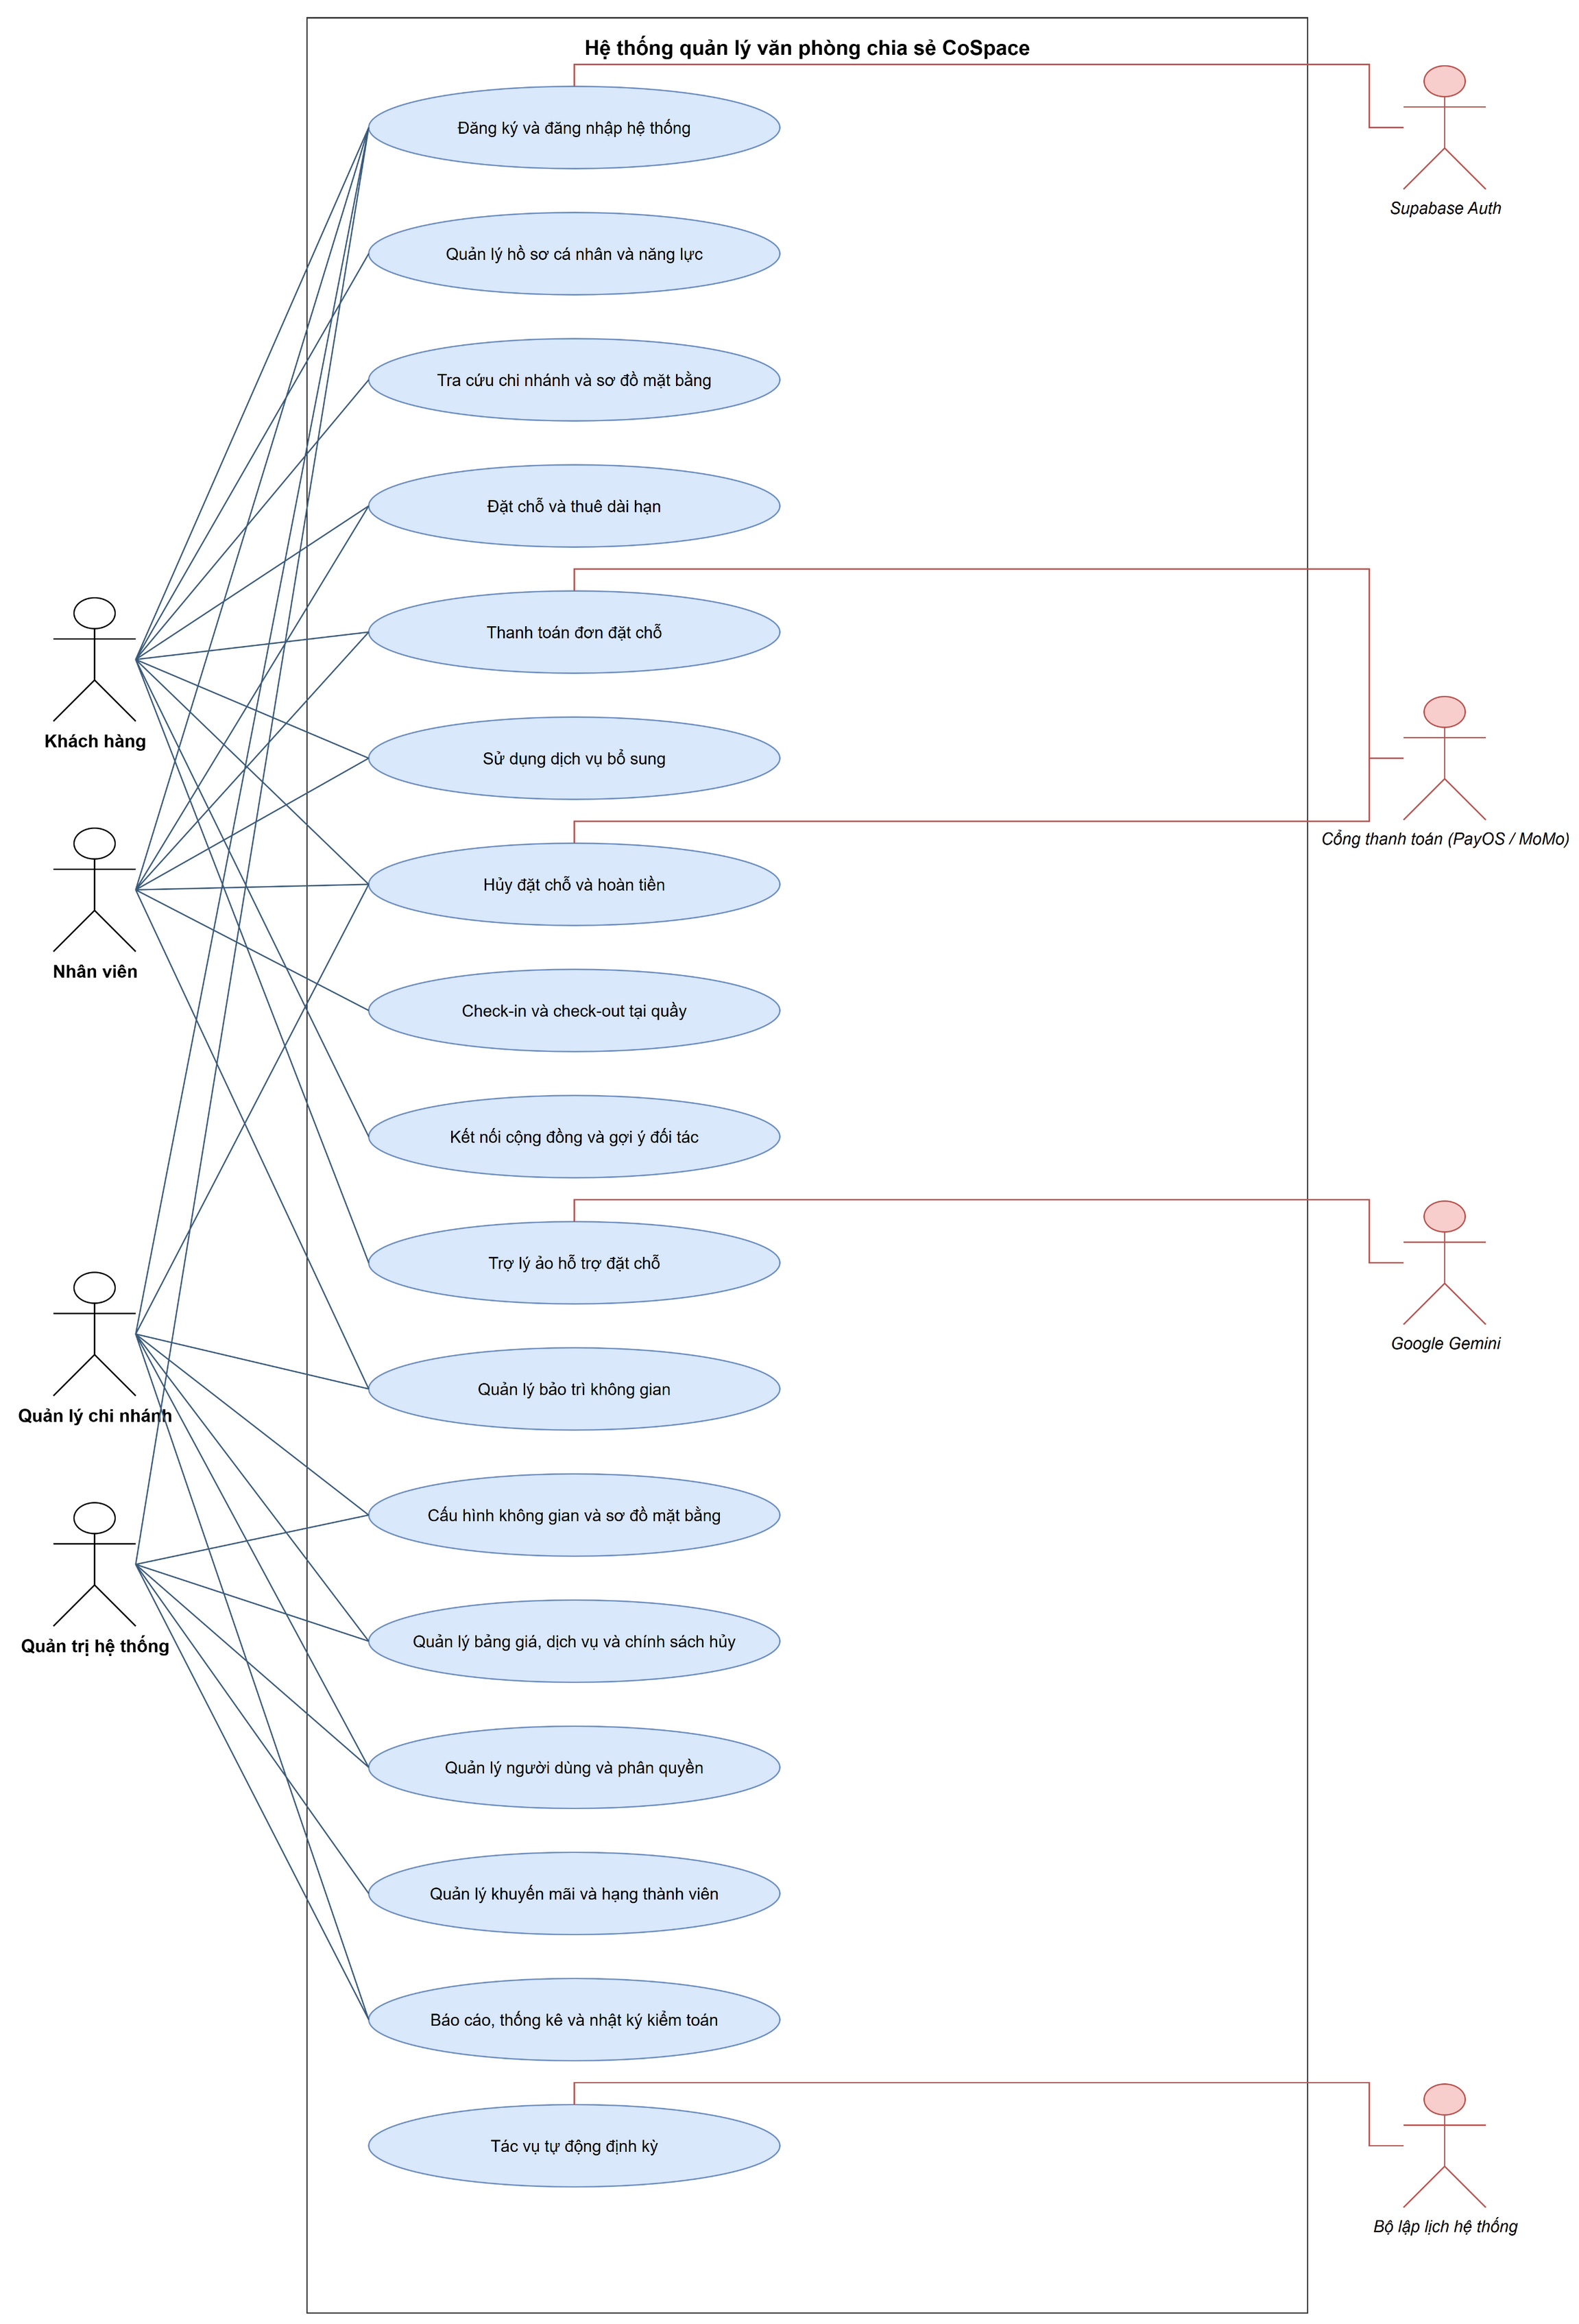
\includegraphics[width=\linewidth,height=0.72\textheight,keepaspectratio]{Chuong5/uc-tongquat.png}
  \caption{Sơ đồ use-case tổng quát của hệ thống quản lý văn phòng chia sẻ CoSpace}
  \label{fig:uc_tongquat}
\end{figure}

Như được thể hiện trên sơ đồ:
\begin{itemize}
    \item Tác nhân **Khách hàng** tương tác chủ yếu với các use-case thuộc phân hệ Đặt chỗ, Thanh toán trực tuyến, Quản lý lịch sử, Xem sơ đồ mặt bằng, Quản lý hồ sơ kết nối đối tác và Trợ lý ảo AI.
    \item Tác nhân **Nhân viên** phụ trách nhóm use-case phục vụ tại quầy: Đặt chỗ cho khách vãng lai, Thu tiền mặt, Check-in/out, Ghi nhận dịch vụ gọi thêm và Báo cáo bảo trì.
    \item Tác nhân **Quản lý chi nhánh** thực hiện các use-case Quản trị không gian, Chỉnh sửa sơ đồ SVG, Thiết lập giá và chính sách hủy của chi nhánh, Quản lý nhân viên cơ sở và Duyệt hoàn tiền.
    \item Tác nhân **Quản trị viên hệ thống** điều phối toàn chuỗi thông qua các use-case Quản lý chi nhánh, Cấu hình danh mục dùng chung, Phân quyền người dùng, Quản lý khuyến mãi, Báo cáo hợp nhất và Tra cứu kiểm toán.
\end{itemize}

\section{Ma trận phân quyền chức năng}
\label{sec:ma_tran_phan_quyen}

Để làm cơ sở cấu hình bảo mật ở tầng ứng dụng và kiểm thử phân quyền, Bảng \ref{tab:matran_phanquyen} mô tả chi tiết ma trận phân quyền (CRUD: Create, Read, Update, Delete) của bốn vai trò đối với từng nhóm tài nguyên dữ liệu trong hệ thống.

\begin{table}[H]
\centering
\caption{Ma trận phân quyền chức năng theo vai trò trong hệ thống CoSpace}
\label{tab:matran_phanquyen}
\small
\renewcommand{\arraystretch}{1.2}
\begin{tabular}{|p{4.0cm}|c|c|c|c|}
\hline
\textbf{Nhóm tài nguyên dữ liệu} & \textbf{Khách hàng} & \textbf{Nhân viên quầy} & \textbf{Quản lý chi nhánh} & \textbf{Quản trị hệ thống} \\
\hline
Xem thông tin chi nhánh, không gian & R & R (chi nhánh) & R (chi nhánh) & CRUD \\
\hline
Cấu hình không gian, tầng, sơ đồ SVG & --- & --- & CRUD (chi nhánh) & CRUD \\
\hline
Đơn đặt chỗ trực tuyến của mình & CRUD & --- & --- & R \\
\hline
Tạo đơn tại quầy cho khách vãng lai & --- & CR (chi nhánh) & CR (chi nhánh) & CR \\
\hline
Xác nhận thanh toán tiền mặt & --- & U (chi nhánh) & U (chi nhánh) & U \\
\hline
Thực hiện Check-in / Check-out & --- & U (chi nhánh) & U (chi nhánh) & U \\
\hline
Ghi nhận dịch vụ phát sinh & --- & CR (chi nhánh) & CR (chi nhánh) & CRUD \\
\hline
Lịch bảo trì cơ sở vật chất & --- & CR (chi nhánh) & CRUD (chi nhánh) & CRUD \\
\hline
Cấu hình bảng giá và chính sách hủy & --- & --- & CRUD (riêng CN) & CRUD (toàn cục) \\
\hline
Hàng chờ phê duyệt hoàn tiền & --- & --- & RU (chi nhánh) & CRUD \\
\hline
Quản lý người dùng và phân quyền & --- & --- & R (NV cơ sở) & CRUD \\
\hline
Báo cáo kinh doanh và xuất CSV & --- & R (trực ban ngày) & R (báo cáo CN) & R (hợp nhất) \\
\hline
Hồ sơ năng lực và gợi ý đối tác & CRUD (cá nhân) & --- & --- & R \\
\hline
Trợ lý ảo AI & CRUD & --- & --- & --- \\
\hline
Nhật ký kiểm toán (Audit Log) & --- & --- & --- & R (toàn hệ thống) \\
\hline
\end{tabular}
\end{table}

\noindent\textit{Ghi chú:} Ký hiệu \textbf{C} (Create -- Tạo mới), \textbf{R} (Read -- Đọc/Xem), \textbf{U} (Update -- Cập nhật), \textbf{D} (Delete -- Xóa/Vô hiệu hóa). Các mục có chú thích ``(chi nhánh)'' biểu thị quyền hạn bị giới hạn nghiêm ngặt trong phạm vi cơ sở mà nhân sự đó đang công tác.

\chapter{Mô hình hóa và đặc tả use-case}
\label{ch:usecase}

\ghichu{Chương này là phần dài nhất của báo cáo phân tích. Mỗi phân hệ gồm: sơ đồ use-case, bảng danh sách use-case, và đặc tả chi tiết cho các use-case quan trọng. Các use-case đơn giản (xem danh sách, xem chi tiết) có thể gom vào một bảng tóm tắt thay vì đặc tả đầy đủ. Dung lượng đề xuất 25--35 trang.}

\section{Quy ước đặc tả use-case}
\label{sec:quyuoc_uc}
\ghichu{Nêu khuôn đặc tả áp dụng thống nhất cho toàn chương: mã use-case, tên, tác nhân, mô tả, điều kiện kích hoạt, tiền điều kiện, hậu điều kiện, luồng sự kiện chính, các luồng thay thế, luồng ngoại lệ, quy tắc nghiệp vụ liên quan. Đưa một bảng mẫu ngay tại đây để người đọc nắm cấu trúc trước khi đọc hàng chục bảng phía sau.}
\nguon{report/Contents/DacTaUseCase.tex (ban Do an chuyen nganh), docs/use\_cases/}
\bangcho{Khuôn mẫu đặc tả chi tiết một use-case}{tab:uc_template}

\section{Phân hệ khách hàng}
\label{sec:uc_customer}
\hinhcho{0.85}{Sơ đồ use-case phân hệ khách hàng}{fig:uc_customer}
\ghichu{Đặc tả các use-case sau, mỗi use-case một bảng: đăng ký tài khoản; đăng nhập; cập nhật hồ sơ cá nhân và hồ sơ năng lực; tra cứu chi nhánh và sơ đồ mặt bằng; tìm kiếm và đặt chỗ; thanh toán đơn đặt chỗ; chọn dịch vụ bổ sung; xem lịch sử đặt chỗ; gửi yêu cầu hủy; xem gợi ý đối tác; tương tác bảng tin cộng đồng; tra cứu điểm tích lũy; đặt chỗ qua trợ lý ảo.}

\subsection{Danh sách use-case của phân hệ}
\subsection{Đặc tả use-case Đăng ký tài khoản}
\subsection{Đặc tả use-case Đăng nhập}
\subsection{Đặc tả use-case Tìm kiếm và đặt chỗ}
\subsection{Đặc tả use-case Thanh toán đơn đặt chỗ}
\subsection{Đặc tả use-case Hủy đặt chỗ và nhận hoàn tiền}
\subsection{Đặc tả use-case Xem gợi ý kết nối đối tác}
\subsection{Đặc tả use-case Đặt chỗ thông qua trợ lý ảo}

\section{Phân hệ nhân viên}
\label{sec:uc_staff}
\hinhcho{0.85}{Sơ đồ use-case phân hệ nhân viên}{fig:uc_staff}

\subsection{Danh sách use-case của phân hệ}
\subsection{Đặc tả use-case Tạo đơn đặt chỗ tại quầy}
\subsection{Đặc tả use-case Xác nhận thanh toán tiền mặt}
\subsection{Đặc tả use-case Check-in và check-out cho khách}
\subsection{Đặc tả use-case Ghi nhận dịch vụ gọi thêm}
\subsection{Đặc tả use-case Quản lý lịch bảo trì không gian}

\section{Phân hệ quản lý chi nhánh}
\label{sec:uc_branchadmin}
\hinhcho{0.85}{Sơ đồ use-case phân hệ quản lý chi nhánh}{fig:uc_branchadmin}

\subsection{Danh sách use-case của phân hệ}
\subsection{Đặc tả use-case Cấu hình không gian và sơ đồ mặt bằng}
\subsection{Đặc tả use-case Thiết lập bảng giá và biểu phí hủy}
\subsection{Đặc tả use-case Quản lý tài khoản nhân viên}
\subsection{Đặc tả use-case Xem báo cáo và xuất dữ liệu}

\section{Phân hệ quản trị hệ thống}
\label{sec:uc_admin}
\hinhcho{0.85}{Sơ đồ use-case phân hệ quản trị hệ thống}{fig:uc_admin}

\subsection{Danh sách use-case của phân hệ}
\subsection{Đặc tả use-case Quản lý chi nhánh và danh mục dùng chung}
\subsection{Đặc tả use-case Quản lý người dùng và phân quyền}
\subsection{Đặc tả use-case Thiết lập chính sách mặc định toàn hệ thống}
\subsection{Đặc tả use-case Tra cứu nhật ký kiểm toán}

\section{Mô hình hóa quy trình nghiệp vụ}
\label{sec:activity}
\ghichu{Vẽ sơ đồ hoạt động cho các quy trình có nhiều nhánh rẽ và nhiều tác nhân tham gia. Mỗi sơ đồ kèm một đoạn diễn giải các nhánh quan trọng, đặc biệt là nhánh lỗi.}

\subsection{Quy trình đặt chỗ và thanh toán trực tuyến}
\hinhcho{0.8}{Sơ đồ hoạt động quy trình đặt chỗ và thanh toán trực tuyến}{fig:act_booking}

\subsection{Quy trình đặt chỗ tại quầy và thanh toán tiền mặt}
\hinhcho{0.8}{Sơ đồ hoạt động quy trình đặt chỗ tại quầy}{fig:act_counter}

\subsection{Quy trình check-in và check-out}
\hinhcho{0.8}{Sơ đồ hoạt động quy trình check-in và check-out}{fig:act_checkin}

\subsection{Quy trình hủy đặt chỗ và hoàn tiền tự động}
\hinhcho{0.8}{Sơ đồ hoạt động quy trình hủy và hoàn tiền}{fig:act_cancel}

\subsection{Quy trình bảo trì không gian và xử lý đơn bị ảnh hưởng}
\hinhcho{0.8}{Sơ đồ hoạt động quy trình bảo trì không gian}{fig:act_maintenance}

\section{Mô hình hóa tương tác giữa các thành phần}
\label{sec:sequence}
\ghichu{Vẽ sơ đồ tuần tự cho các luồng kỹ thuật cần thể hiện thứ tự thời gian và ranh giới giao dịch: luồng xin khóa tư vấn rồi kiểm tra chồng lấn khi tạo đơn; luồng nhận webhook từ cổng thanh toán và cập nhật trạng thái; luồng tác vụ định kỳ quét đơn quá hạn thanh toán; luồng trợ lý ảo gọi hàm nghiệp vụ.}

\subsection{Luồng tạo đơn đặt chỗ có khóa chống tương tranh}
\hinhcho{0.8}{Sơ đồ tuần tự luồng tạo đơn đặt chỗ}{fig:seq_booking}

\subsection{Luồng xử lý thông báo kết quả thanh toán}
\hinhcho{0.8}{Sơ đồ tuần tự luồng xử lý webhook thanh toán}{fig:seq_webhook}

\section{Mô hình trạng thái}
\label{sec:statechart}
\ghichu{Vẽ sơ đồ trạng thái cho đơn đặt chỗ và cho giao dịch thanh toán, kèm bảng liệt kê điều kiện chuyển trạng thái và tác nhân gây ra chuyển trạng thái. Đây là căn cứ để kiểm thử máy trạng thái ở Chương \ref{ch:kiemthu}.}
\nguon{docs/SYSTEM\_SPEC.md muc 3.3 va 3.4}
\hinhcho{0.8}{Sơ đồ trạng thái của đơn đặt chỗ}{fig:state_booking}
\hinhcho{0.8}{Sơ đồ trạng thái của giao dịch thanh toán}{fig:state_payment}

\chapter{Kiến trúc và thiết kế hệ thống}
\label{ch:thietke}

\section{Kiến trúc tổng thể}
\label{sec:kientruc}

Hệ thống CoSpace được thiết kế theo mô hình kiến trúc khách--chủ ba tầng (Client--Server 3-Tier Architecture) kết hợp kiến trúc hướng dịch vụ nội bộ tinh gọn. Toàn bộ các thành phần của hệ thống và các kênh giao tiếp liên tầng được thể hiện tại Hình \ref{fig:kientruc_tongthe}.

\hinhdo{Chuong6/arch-tongthe}{Kiến trúc tổng thể của hệ thống CoSpace}{fig:kientruc_tongthe}

Kiến trúc bao gồm ba tầng chính và các dịch vụ tích hợp bên ngoài:
\begin{enumerate}
    \item \textbf{Tầng trình bày (Presentation Tier -- Front-end):} Ứng dụng Single Page Application (SPA) xây dựng trên React 18 và TypeScript, được đóng gói tối ưu bằng Vite và phân phối qua mạng lưới máy chủ biên Vercel Edge CDN. Người dùng cuối giao tiếp với ứng dụng thông qua trình duyệt web trên máy tính hoặc thiết bị di động.
    \item \textbf{Tầng ứng dụng (Application Tier -- Back-end):} Máy chủ ứng dụng Spring Boot 3 đóng gói trong Docker container và vận hành trên nền tảng đám mây Render. Máy chủ tiếp nhận các yêu cầu HTTPS từ Front-end, chịu trách nhiệm xử lý logic nghiệp vụ, quản lý giao dịch ACID, phân quyền bảo mật và điều phối tương tranh.
    \item \textbf{Tầng dữ liệu (Data Tier -- Database):} Hệ quản trị cơ sở dữ liệu quan hệ PostgreSQL vận hành trên nền tảng đám mây Supabase tại khu vực Châu Á. Tầng ứng dụng kết nối trực tiếp đến PostgreSQL thông qua giao thức JDBC với bể kết nối HikariCP được mã hóa SSL (cổng 6543).
    \item \textbf{Các dịch vụ đám mây tích hợp bên thứ ba:}
    \begin{itemize}
        \item \textit{Supabase Auth:} Đảm nhận xác thực đăng nhập một lần (Google SSO) và cấp phát thẻ xác thực OAuth2.
        \item \textit{PayOS:} Cổng thanh toán quốc gia VietQR Napas 24/7, phát hành mã QR động và gửi tín hiệu xác nhận qua Webhook.
        \item \textit{Ví điện tử MoMo:} Cung cấp kênh thanh toán ví điện tử thử nghiệm qua giao thức IPN Webhook.
        \item \textit{Google Gemini AI:} Mô hình ngôn ngữ lớn cung cấp dịch vụ trí tuệ nhân tạo đàm thoại và gọi hàm công cụ qua luồng dữ liệu một chiều SSE (Server-Sent Events).
    \end{itemize}
\end{enumerate}

\subsection{Kiến trúc phân tầng phía máy chủ}
\label{ssec:phantang_be}
Mã nguồn Back-end được tổ chức thành các gói tính năng theo mô hình phân lớp chuẩn mực của Spring Boot:
\begin{itemize}
    \item \textbf{Gói \texttt{controller}:} Gồm 26 lớp điều khiển RESTful đón nhận các yêu cầu HTTP. Controller chỉ đóng vai trò phân tích tham số, xác thực dữ liệu đầu vào (Bean Validation) và ủy quyền xử lý cho tầng dịch vụ.
    \item \textbf{Gói \texttt{service}:} Gồm 32 lớp dịch vụ nghiệp vụ (trong đó 23 lớp được quản lý giao dịch khai báo bằng chú thích \texttt{@Transactional}). Điểm cốt lõi là sự hiện diện của lớp \texttt{BookingStateMachine} -- cổng kiểm soát duy nhất cho mọi chuyển đổi trạng thái của đơn đặt chỗ, ngăn ngừa hoàn toàn các chuyển trạng thái vi phạm quy tắc.
    \item \textbf{Gói \texttt{repository}:} Gồm 29 giao diện kế thừa \texttt{JpaRepository}, cung cấp các phương thức truy vấn tối ưu và các câu lệnh khóa dòng dữ liệu bi quan (\texttt{findByIdWithLock}).
    \item \textbf{Gói \texttt{entity}:} Gồm 29 lớp thực thể đại diện cho cấu trúc 30 bảng trong cơ sở dữ liệu quan hệ.
    \item \textbf{Gói \texttt{security}:} Chứa các thành phần xác thực và phân quyền: \texttt{SecurityConfig}, \texttt{SupabaseJwtAuthenticationConverter}, \texttt{BranchAccessGuard} và \texttt{JwtUtil}.
\end{itemize}

\subsection{Kiến trúc phía giao diện người dùng}
\label{ssec:phantang_fe}
Ứng dụng Front-end được cấu trúc theo định hướng mô-đun hóa chức năng (Feature-based structure) như minh họa tại Hình \ref{fig:kientruc_frontend}.

\hinhdongang{Chuong6/arch-frontend}{Kiến trúc phía giao diện người dùng của hệ thống CoSpace}{fig:kientruc_frontend}

Các thành phần kiến trúc chính bao gồm:
\begin{itemize}
    \item \textbf{Tầng truy cập API tập trung (\texttt{src/api/}):} Đóng gói toàn bộ các hàm gọi HTTP thông qua một đối tượng Axios/Fetch duy nhất (\texttt{api.ts}). Mã nguồn tự động gắn thẻ Bearer Token vào tiêu đề \texttt{Authorization}, tự động bắt lỗi \texttt{401 Unauthorized} để làm mới token thông qua Refresh Token và định hình kiểu trả về chuẩn xác theo TypeScript DTO.
    \item \textbf{Bộ quản lý trạng thái xác thực toàn cục (\texttt{AuthContext}):} Lưu trữ thông tin định danh của người dùng hiện tại, trạng thái đăng nhập, vai trò và định danh chi nhánh.
    \item \textbf{Định tuyến phân quyền theo vai trò (\texttt{ProtectedRoute}):} Kiểm soát nghiêm ngặt việc truy cập đường dẫn dựa trên vai trò người dùng, tự động chuyển hướng khách hàng về đúng trang chủ của vai trò đó sau khi đăng nhập thành công.
    \item \textbf{Tải lười (Lazy Loading) và chia nhỏ gói mã (Code Splitting):} Sử dụng hàm \texttt{React.lazy()} cho toàn bộ 34 mô-đun trang, kết hợp với cấu hình chia nhỏ thư viện của Vite (\texttt{manualChunks}) giúp giảm dung lượng tải trang lần đầu xuống dưới 300KB.
\end{itemize}

\subsection{Triển khai và môi trường vận hành}
\label{ssec:trienkhai_tong}
Hệ thống được phát hành và vận hành theo mô hình kiến trúc đám mây đa nền tảng (Multi-cloud Architecture), tách biệt giữa việc phân phối tệp tĩnh và thực thi mã nghiệp vụ (Hình \ref{fig:trienkhai}).

\hinhdo{Chuong6/arch-trienkhai}{Sơ đồ triển khai của hệ thống CoSpace}{fig:trienkhai}

\section{Thiết kế lớp}
\label{sec:thietke_lop}

\noindent\textbf{Quy ước đọc sơ đồ lớp trong đề tài:}
\begin{itemize}
    \item \textbf{Khóa ngoại UUID thuần túy:} Các lớp thực thể trong CoSpace sử dụng thuộc tính khóa ngoại kiểu \texttt{UUID} (được đánh dấu ký hiệu \guillemotleft FK\guillemotright) thay vì khai báo quan hệ đối tượng \texttt{@ManyToOne} hay \texttt{@OneToMany} của Hibernate. Quan hệ giữa các lớp được thể hiện bằng đường liên kết có chỉ số bội số ($1..1$, $0..*$). Quyết định thiết kế này giúp loại bỏ hoàn toàn các lỗi tải lười (LazyInitializationException) và truy vấn thừa $N+1$, giữ các lớp thực thể đơn giản và tăng tính trong sáng khi viết câu lệnh SQL tường minh.
    \item \textbf{Quan hệ kết tập mạnh (Composition):} Biểu thị bằng hình thoi đặc, thể hiện vòng đời của đối tượng con phụ thuộc hoàn toàn vào đối tượng cha (ví dụ: \texttt{BookingAddon} phụ thuộc \texttt{Booking}).
    \item \textbf{Quan hệ phụ thuộc (Dependency):} Biểu thị bằng mũi tên đứt nét, thể hiện sự trao đổi dữ liệu hoặc lời gọi phương thức giữa các lớp dịch vụ.
    \item \textbf{Hộp lớp nét đứt in nghiêng:} Biểu thị các lớp ngoại vi hoặc các lớp đã được định nghĩa chi tiết ở một sơ đồ khác. Các trường thời gian hệ thống (\texttt{createdAt}, \texttt{updatedAt}) được lược bỏ ở mọi lớp để sơ đồ đạt độ trực quan cao nhất.
\end{itemize}

\subsection{Mô hình miền dữ liệu (Domain Model Classes)}
\label{ssec:lop_mien}

Mô hình miền dữ liệu của hệ thống CoSpace được tổ chức thành 6 sơ đồ lớp nghiệp vụ chuyên biệt:

\subsubsection{1. Miền Không gian làm việc (Hình \ref{fig:cd_khonggian})}
Sơ đồ phản ánh cấu trúc phân cấp vật lý: Chi nhánh (\texttt{Branch}) $\rightarrow$ Tầng (\texttt{Floor}) $\rightarrow$ Không gian làm việc (\texttt{Workspace}). Điểm đặc sắc là lớp liên kết \texttt{WorkspaceTypeAmenity}: các tiện ích (\texttt{Amenity}) được gắn kết ở mức Loại không gian (\texttt{WorkspaceType}), nhờ đó mọi không gian làm việc thuộc cùng một loại sẽ tự động thừa hưởng toàn bộ danh mục tiện ích tương ứng.

\hinhuml{cd-01-khonggian}{Sơ đồ lớp miền dữ liệu: không gian làm việc}{fig:cd_khonggian}

\subsubsection{2. Miền Bảng giá, Dịch vụ bổ sung và Chính sách hủy (Hình \ref{fig:cd_gia})}
Sơ đồ thể hiện mô hình kế thừa ``Toàn cục và ghi đè theo chi nhánh'' (Global with Branch Override). Các thực thể \texttt{PricePolicy}, \texttt{ExtraService} và \texttt{CancellationPolicy} đều chứa trường \texttt{branchId} có thể nhận giá trị rỗng (\texttt{NULL}). Nếu \texttt{branchId} là \texttt{NULL}, chính sách đó có hiệu lực toàn hệ thống; nếu có giá trị cụ thể, chính sách đó là độc quyền của chi nhánh và được ưu tiên áp dụng trước.

\hinhuml{cd-02-gia-chinhsach}{Sơ đồ lớp miền dữ liệu: bảng giá, dịch vụ bổ sung và chính sách hủy}{fig:cd_gia}

\subsubsection{3. Miền Đặt chỗ, Check-in và Hủy phòng (Hình \ref{fig:cd_datcho})}
Đây là sơ đồ trung tâm của hệ thống. Lớp \texttt{Booking} đóng vai trò quản lý vòng đời đơn với 4 thuộc tính tài chính độc lập: \texttt{subtotalAmount} (tiền thuê không gian), \texttt{discountAmount} (tiền giảm giá ưu đãi), \texttt{extraServicesAmount} (tiền dịch vụ phát sinh) và \texttt{totalAmount} (tổng tiền thanh toán). Lớp \texttt{BookingAddon} lưu trữ bản chụp đơn giá (\texttt{unitPrice}) tại thời điểm phát sinh dịch vụ, đảm bảo việc điều chỉnh giá dịch vụ sau này không làm thay đổi các hóa đơn cũ. Lớp \texttt{BookingCheckin} cho phép tạo nhiều lượt check-in mở/đóng phục vụ các gói thuê dài hạn nhiều ngày.

\hinhuml{cd-03-datcho}{Sơ đồ lớp miền dữ liệu: đặt chỗ, check-in và hủy}{fig:cd_datcho}

\subsubsection{4. Miền Thanh toán, Hoàn tiền và Ưu đãi thành viên (Hình \ref{fig:cd_thanhtoan})}
Một đơn đặt chỗ có thể có nhiều giao dịch thanh toán (\texttt{Payment}). Thực thể \texttt{RefundRequest} đại diện cho yêu cầu hoàn tiền độc lập, được tạo ra khi đơn bị hủy hoặc khi khách thanh toán muộn, chỉ có thể được duyệt bởi Quản lý chi nhánh hoặc Quản trị viên. Lớp \texttt{UserLoyalty} theo dõi tổng chi tiêu thực tế để xếp hạng hội viên theo các ngưỡng cấu hình trong \texttt{MembershipTier}.

\hinhuml{cd-04-thanhtoan}{Sơ đồ lớp miền dữ liệu: thanh toán, hoàn tiền, khuyến mãi và hạng thành viên}{fig:cd_thanhtoan}

\subsubsection{5. Miền Hồ sơ năng lực và Gợi ý đối tác (Hình \ref{fig:cd_goiy})}
Lớp \texttt{UserProfile} lưu trữ thông tin chuyên môn, liên kết với danh sách kỹ năng (\texttt{UserSkill}) có đánh giá mức độ thành thạo ($1..5$) và danh sách sở thích (\texttt{UserInterest}). Kết quả tính toán độ tương đồng giữa hai thành viên được lưu tạm vào \texttt{PartnerMatch} kèm theo các trường giải thích lý do so khớp dưới dạng JSON.

\hinhuml{cd-05-goiydoitac}{Sơ đồ lớp miền dữ liệu: hồ sơ năng lực và gợi ý đối tác}{fig:cd_goiy}

\subsubsection{6. Miền Cộng đồng, Thông báo và Nhật ký kiểm toán (Hình \ref{fig:cd_congdong})}
Quản lý các bài viết trên diễn đàn (\texttt{Post}), các thẻ phân loại (\texttt{PostTag}), thông báo trong ứng dụng (\texttt{Notification}) và nhật ký kiểm toán bất biến (\texttt{AuditLog}) lưu trữ dấu vết thao tác của người dùng.

\hinhuml{cd-06-congdong}{Sơ đồ lớp miền dữ liệu: bảng tin cộng đồng, thông báo và nhật ký kiểm toán}{fig:cd_congdong}

\subsection{Tầng nghiệp vụ (Service Layer Classes)}
\label{ssec:lop_dichvu}

Tầng dịch vụ nghiệp vụ được thiết kế tuân thủ nguyên lý Trách nhiệm đơn lẻ (Single Responsibility Principle), được mô hình hóa qua 5 sơ đồ lớp dịch vụ:

\subsubsection{1. Tầng dịch vụ Đặt chỗ và Tính giá (Hình \ref{fig:cd_svc_datcho})}
\texttt{BookingService} giữ vai trò nhạc trưởng điều phối việc kiểm tra hạn mức, lấy khóa tư vấn, tính đơn giá qua \texttt{PricingService}, áp dụng giảm giá qua \texttt{LoyaltyService} và chuyển đổi trạng thái an toàn qua \texttt{BookingStateMachine}.

\hinhumlngang{cd-07-svc-datcho}{Sơ đồ lớp tầng nghiệp vụ: đặt chỗ, tính giá và ưu đãi}{fig:cd_svc_datcho}

\subsubsection{2. Tầng dịch vụ Vòng đời tự động, Check-in và Bảo trì (Hình \ref{fig:cd_svc_vongdoi})}
Bao gồm \texttt{BookingLifecycleService}, \texttt{BookingExpiryScheduler} (tác vụ tự động hủy đơn hết hạn 15 phút), \texttt{CheckinService} (xác thực cửa sổ check-in 30 phút) và \texttt{StaffMaintenanceService} (khóa không gian bảo trì và xử lý đơn bị ảnh hưởng).

\hinhuml{cd-08-svc-vongdoi}{Sơ đồ lớp tầng nghiệp vụ: vòng đời tự động, check-in và bảo trì}{fig:cd_svc_vongdoi}

\subsubsection{3. Tầng dịch vụ Thanh toán, Hủy đơn và Hoàn tiền (Hình \ref{fig:cd_svc_thanhtoan})}
Điều phối giao tiếp với cổng PayOS (\texttt{PayosService}), ví MoMo (\texttt{MomoService}), xử lý hủy đơn theo bậc thời gian (\texttt{CancellationService}) và quản lý hàng chờ hoàn tiền (\texttt{RefundService}).

\hinhumlngang{cd-09-svc-thanhtoan}{Sơ đồ lớp tầng nghiệp vụ: thanh toán, hủy và hoàn tiền}{fig:cd_svc_thanhtoan}

\subsubsection{4. Tầng dịch vụ Xác thực và Phân quyền (Hình \ref{fig:cd_svc_xacthuc})}
Bao gồm \texttt{AuthService}, \texttt{JwtUtil} (ký và kiểm tra token HS384), \texttt{SupabaseJwtAuthenticationConverter} (nạp quyền động từ CSDL) và \texttt{BranchAccessGuard} (chốt chặn cô lập dữ liệu chi nhánh).

\hinhuml{cd-10-svc-xacthuc}{Sơ đồ lớp tầng nghiệp vụ: xác thực và phân quyền}{fig:cd_svc_xacthuc}

\subsubsection{5. Tầng dịch vụ Trợ lý ảo AI, Gợi ý đối tác và Kiểm toán (Hình \ref{fig:cd_svc_trolyao})}
Bao gồm \texttt{ChatbotService} (kết nối Gemini API qua \texttt{GeminiClient}, điều phối Function Calling), \texttt{PartnerMatchingService} (tính điểm Jaccard) và \texttt{AuditLogService} (ghi nhận vết an ninh bất đồng bộ).

\hinhuml{cd-11-svc-trolyao}{Sơ đồ lớp tầng nghiệp vụ: trợ lý ảo, gợi ý đối tác và nhật ký kiểm toán}{fig:cd_svc_trolyao}

\clearpage
\section{Thiết kế cơ sở dữ liệu}
\label{sec:thietke_csdl}

Cơ sở dữ liệu của CoSpace được thiết kế ở dạng chuẩn 3NF gồm **30 bảng quan hệ**, được quản lý di trú phiên bản lược đồ bằng Flyway (\texttt{V1\_\_baseline.sql} khởi tạo cấu trúc và \texttt{V2\_\_constraints.sql} bổ sung các ràng buộc toàn vẹn).

\subsection{Sơ đồ quan hệ thực thể tổng quan và các phân hệ}
Bản đồ phân bổ 30 bảng CSDL theo 6 phân hệ chức năng được trình bày tại Hình \ref{fig:erd}.

\hinhdo{Chuong6/erd-00-tongquan}{Bản đồ các module của cơ sở dữ liệu CoSpace (30 bảng)}{fig:erd}

Chi tiết cấu trúc các bảng theo từng phân hệ được thể hiện trong các sơ đồ ERD chuyên sâu:
\begin{itemize}
    \item \textbf{Phân hệ Định danh và Gợi ý đối tác (Hình \ref{fig:erd_dinhdanh}):} Gồm các bảng \texttt{users}, \texttt{user\_profiles}, \texttt{skills}, \texttt{user\_skills}, \texttt{interests}, \texttt{user\_interests}, \texttt{partner\_matches} và \texttt{auth\_accounts}.
    \item \textbf{Phân hệ Không gian làm việc (Hình \ref{fig:erd_khonggian}):} Gồm các bảng \texttt{branches}, \texttt{floors}, \texttt{workspaces}, \texttt{workspace\_types}, \texttt{amenities}, \texttt{workspace\_type\_amenities} và \texttt{workspace\_maintenance}.
    \item \textbf{Phân hệ Giá, Khuyến mãi và Hội viên (Hình \ref{fig:erd_gia}):} Gồm các bảng \texttt{price\_policies}, \texttt{extra\_services}, \texttt{cancellation\_policies}, \texttt{promotions}, \texttt{promotion\_usages}, \texttt{membership\_tiers} và \texttt{user\_loyalty}.
    \item \textbf{Phân hệ Đặt chỗ và Vận hành (Hình \ref{fig:erd_datcho}):} Gồm các bảng \texttt{bookings}, \texttt{booking\_addons}, \texttt{booking\_checkins} và \texttt{booking\_cancellations}.
    \item \textbf{Phân hệ Thanh toán và Hoàn tiền (Hình \ref{fig:erd_thanhtoan}):} Gồm các bảng \texttt{payments}, \texttt{payment\_events} và \texttt{refund\_requests}.
    \item \textbf{Phân hệ Cộng đồng và Kiểm toán (Hình \ref{fig:erd_congdong}):} Gồm các bảng \texttt{posts}, \texttt{post\_tags}, \texttt{notifications} và \texttt{audit\_logs}.
\end{itemize}

\hinhdo{Chuong6/erd-01-dinhdanh}{ERD: định danh, hồ sơ và gợi ý đối tác}{fig:erd_dinhdanh}
\hinhdo{Chuong6/erd-02-khonggian}{ERD: không gian làm việc}{fig:erd_khonggian}
\hinhdo{Chuong6/erd-03-gia}{ERD: bảng giá, dịch vụ bổ sung, chính sách hủy, khuyến mãi và hạng thành viên}{fig:erd_gia}
\hinhdo{Chuong6/erd-04-datcho}{ERD: đặt chỗ, dịch vụ gọi thêm, check-in và hủy}{fig:erd_datcho}
\hinhdo{Chuong6/erd-05-thanhtoan}{ERD: thanh toán và hoàn tiền}{fig:erd_thanhtoan}
\hinhdo{Chuong6/erd-06-congdong}{ERD: bảng tin cộng đồng, thông báo và nhật ký kiểm toán}{fig:erd_congdong}

Bảng \ref{tab:bang_theo_module} thống kê số lượng bảng, khóa chính và vai trò của từng nhóm trong cơ sở dữ liệu.

\begin{table}[H]
\centering
\caption{Thống kê 30 bảng cơ sở dữ liệu theo các phân hệ chức năng}
\label{tab:bang_theo_module}
\small
\renewcommand{\arraystretch}{1.2}
\begin{tabular}{|p{3.8cm}|c|p{8.4cm}|}
\hline
\textbf{Phân hệ chức năng} & \textbf{Số bảng} & \textbf{Danh sách các bảng cơ sở dữ liệu} \\
\hline
Định danh \& Gợi ý đối tác & 8 & \texttt{users}, \texttt{user\_profiles}, \texttt{skills}, \texttt{user\_skills}, \texttt{interests}, \texttt{user\_interests}, \texttt{partner\_matches}, \texttt{auth\_accounts} \\
\hline
Không gian làm việc & 7 & \texttt{branches}, \texttt{floors}, \texttt{workspaces}, \texttt{workspace\_types}, \texttt{amenities}, \texttt{workspace\_type\_amenities}, \texttt{workspace\_maintenance} \\
\hline
Giá, Khuyến mãi \& Hội viên & 7 & \texttt{price\_policies}, \texttt{extra\_services}, \texttt{cancellation\_policies}, \texttt{promotions}, \texttt{promotion\_usages}, \texttt{membership\_tiers}, \texttt{user\_loyalty} \\
\hline
Đặt chỗ \& Vận hành quầy & 4 & \texttt{bookings}, \texttt{booking\_addons}, \texttt{booking\_checkins}, \texttt{booking\_cancellations} \\
\hline
Thanh toán \& Hoàn tiền & 3 & \texttt{payments}, \texttt{payment\_events}, \texttt{refund\_requests} \\
\hline
Cộng đồng \& Kiểm toán & 4 & \texttt{posts}, \texttt{post\_tags}, \texttt{notifications}, \texttt{audit\_logs} \\
\hline
\textbf{Tổng cộng} & \textbf{30} & Quản lý bằng Flyway Migration (\texttt{V1}, \texttt{V2}) \\
\hline
\end{tabular}
\end{table}

\subsection{Các ràng buộc toàn vẹn dữ liệu quan trọng}
\begin{itemize}
    \item \textbf{Ràng buộc loại trừ khoảng thời gian (EXCLUDE constraint):} Trên bảng \texttt{bookings} và \texttt{workspace\_maintenance}, ràng buộc \texttt{EXCLUDE USING gist (workspace\_id WITH =, tstzrange(start\_at, end\_at) WITH \&\&)} ngăn chặn hoàn toàn việc chèn hai bản ghi có khoảng thời gian giao nhau trên cùng một không gian.
    \item \textbf{Ràng buộc đẳng thức tổng tiền:} Bảng \texttt{bookings} có ràng buộc kiểm tra \texttt{CHECK (total\_amount = subtotal\_amount - discount\_amount + extra\_services\_amount)} và \texttt{CHECK (total\_amount >= 0)}.
    \item \textbf{Ràng buộc logic thời gian:} \texttt{CHECK (end\_at > start\_at)} trên toàn bộ các bảng có dữ liệu khoảng thời gian (\texttt{bookings}, \texttt{workspace\_maintenance}, \texttt{price\_policies}, \texttt{promotions}).
    \item \textbf{Ràng buộc vai trò và chi nhánh:} \texttt{CHECK (role IN ('customer', 'super\_admin') OR branch\_id IS NOT NULL)} trên bảng \texttt{users}.
\end{itemize}

\section{Thiết kế giao diện lập trình ứng dụng}
\label{sec:thietke_api}

Hệ thống cung cấp **133 điểm cuối API** được tổ chức thành 26 lớp điều khiển RESTful, tuân thủ các quy chuẩn thiết kế:
\begin{itemize}
    \item \textbf{Phân nhóm đường dẫn theo cấp độ bảo mật:} \texttt{/api/public/**} (công khai không cần đăng nhập), \texttt{/api/customer/**} (dành cho khách hàng), \texttt{/api/staff/**} (dành cho nhân viên quầy), \texttt{/api/branch-admin/**} (dành cho quản lý cơ sở), \texttt{/api/admin/**} (dành cho quản trị viên tối cao).
    \item \textbf{Tiêu đề chống lặp (\texttt{Idempotency-Key}):} Bắt buộc áp dụng cho các điểm cuối tạo giao dịch thanh toán để ngăn chặn việc gửi đúp yêu cầu từ máy khách.
    \item \textbf{Luồng dữ liệu thời gian thực (SSE Stream):} Điểm cuối \texttt{/api/customer/chatbot/stream} sử dụng chuẩn Server-Sent Events để truyền từng phần câu trả lời của mô hình ngôn ngữ lớn đến trình duyệt.
\end{itemize}

Bảng \ref{tab:api_nhom} tóm tắt các nhóm điểm cuối API chính và vai trò được phép truy cập tương ứng.

\begin{table}[H]
\centering
\caption{Các nhóm điểm cuối API và vai trò được phép truy cập trong hệ thống}
\label{tab:api_nhom}
\small
\renewcommand{\arraystretch}{1.2}
\begin{tabular}{|p{4.2cm}|p{4.8cm}|p{4.8cm}|}
\hline
\textbf{Nhóm chức năng API} & \textbf{Tiền tố đường dẫn (Base URI)} & \textbf{Vai trò được phép truy cập} \\
\hline
Xác thực \& Đăng nhập & \texttt{/api/auth/**} & Công khai (Public) \\
\hline
Tra cứu chi nhánh \& Mặt bằng & \texttt{/api/branches/**}, \texttt{/api/spaces/**} & Công khai (chỉ xem thông tin hoạt động) \\
\hline
Đặt chỗ của khách hàng & \texttt{/api/customer/bookings/**} & Khách hàng (\texttt{customer}) \\
\hline
Thanh toán trực tuyến \& Webhook & \texttt{/api/payments/**} & Khách hàng; Webhook công khai (kiểm tra chữ ký) \\
\hline
Hồ sơ, Gợi ý đối tác, Bảng tin & \texttt{/api/customer/profile/**}, \texttt{community} & Khách hàng (\texttt{customer}) \\
\hline
Trợ lý ảo AI đàm thoại & \texttt{/api/customer/chatbot/**} & Khách hàng (\texttt{customer}) \\
\hline
Vận hành quầy (Check-in, Walk-in) & \texttt{/api/staff/**}, \texttt{/api/checkins/**} & Nhân viên, Quản lý chi nhánh, Super Admin \\
\hline
Cấu hình chi nhánh \& Mặt bằng & \texttt{/api/branch-admin/spaces/**} & Quản lý chi nhánh, Super Admin \\
\hline
Hàng chờ phê duyệt hoàn tiền & \texttt{/api/refunds/**} & Quản lý chi nhánh, Super Admin \\
\hline
Báo cáo doanh thu chi nhánh & \texttt{/api/reports/**} & Quản lý chi nhánh, Super Admin \\
\hline
Quản trị toàn hệ thống \& Kiểm toán & \texttt{/api/admin/**} & Quản trị hệ thống (\texttt{super\_admin}) \\
\hline
\end{tabular}
\end{table}

\section{Thiết kế bảo mật}
\label{sec:thietke_baomat}

Kiến trúc bảo mật của CoSpace được thiết kế theo nguyên lý **phòng thủ theo chiều sâu (Defense-in-Depth)** gồm 7 lớp bảo vệ:
\begin{enumerate}
    \item \textbf{Mã hóa đường truyền (Transport Layer Security):} Bắt buộc toàn bộ lưu lượng giao tiếp giữa trình duyệt, máy chủ API và cơ sở dữ liệu đều qua giao thức HTTPS với chuẩn mã hóa TLS 1.3.
    \item \textbf{Xác thực kép và thu hồi quyền tức thì:} Kết hợp Supabase JWT và JWT nội bộ ký HS384. Tại mỗi yêu cầu, \texttt{SupabaseJwtAuthenticationConverter} truy vấn lại trạng thái tài khoản từ CSDL; nếu tài khoản bị vô hiệu hóa, quyền truy cập bị ngắt ngay lập tức.
    \item \textbf{Kiểm soát truy cập theo vai trò (RBAC):} Phân quyền kép tại cấu hình bảo mật đường dẫn (\texttt{SecurityConfig}) và tại mức phương thức thông qua các chú thích \texttt{@PreAuthorize("hasRole('BRANCH\_ADMIN')")}.
    \item \textbf{Cô lập dữ liệu đa chi nhánh (\texttt{BranchAccessGuard}):} Mọi yêu cầu liên quan đến tài nguyên của một chi nhánh đều phải đi qua bộ chốt chặn \texttt{BranchAccessGuard}. Bộ chốt chặn so khớp mã định danh \texttt{branch\_id} của tài khoản đang đăng nhập với \texttt{branch\_id} của tài nguyên; người dùng chỉ được thao tác trên đúng cơ sở của mình, ngoại trừ Super Admin.
    \item \textbf{Xác thực chữ ký số Webhook thanh toán:} Thông báo Webhook từ cổng PayOS và MoMo bắt buộc phải đi kèm chữ ký mật mã HMAC-SHA256. Máy chủ tính toán lại chữ ký bằng khóa bí mật và thực hiện so sánh chuỗi bằng thuật toán thời gian hằng số (Constant-time comparison) để triệt tiêu nguy cơ tấn công kênh kề (Timing attack).
    \item \textbf{Phòng thủ tấn công tiêm mã (Injection \& XSS Defense):} Spring Data JPA sử dụng các câu lệnh Parameterized Queries loại trừ hoàn toàn nguy cơ SQL Injection. Phía Front-end sử dụng thư viện DOMPurify để làm sạch mã HTML trước khi hiển thị trên diễn đàn cộng đồng, kết hợp với các chính sách bảo mật nội dung (Content Security Policy -- CSP) nghiêm ngặt cấu hình trên Vercel.
    \item \textbf{Chốt chặn an toàn môi trường phát hành (\texttt{PayosProductionGuard}):} Khi máy chủ khởi động ở cấu hình Production (\texttt{application-prod.yml}), hệ thống tự động kiểm tra các khóa cấu hình PayOS. Nếu phát hiện hệ thống đang chạy ở chế độ giả lập hoặc thiếu thông tin bảo mật thật, máy chủ sẽ chủ động từ chối khởi động nhằm ngăn ngừa rủi ro thất thoát doanh thu ngoài ý muốn.
\end{enumerate}

\chapter{Hiện thực hệ thống}
\label{ch:hienthuc}

\ghichu{Chương này cho thấy thiết kế ở Chương \ref{ch:thietke} được biến thành mã như thế nào và những kỹ thuật nào bảo đảm các yêu cầu khó nhất: đúng đắn khi tương tranh, an toàn tiền, bảo mật. Không dán mã dài. Mỗi thành phần gồm trách nhiệm, bảng đặc tả phương thức và các bước thuật toán; đoạn mã chỉ dùng cho hai hoặc ba kỹ thuật then chốt, mỗi đoạn tối đa 12 dòng. Dung lượng đề xuất 22--30 trang. Các số liệu trong chương được đo ngày 21/09/2026 trên nhánh \texttt{feat/architecture-optimization-and-fixes}; nếu mã thay đổi thì đo lại.}

\section{Môi trường phát triển và công cụ}
\label{sec:ht_moitruong}

\subsection{Công nghệ và phiên bản sử dụng}
\label{ssec:ht_congnghe}
\ghichu{Chỉ ghi phiên bản có thật trong tệp cấu hình, không ghi theo trí nhớ. Các điểm dễ sai: mã được biên dịch ở mức Java 17 nhưng ảnh Docker chạy trên JRE 21; \texttt{pom.xml} khai báo Spring Boot 3.1.12 ở phần \texttt{parent} (thuộc tính \texttt{spring.boot.version} 3.1.6 chỉ dùng cho plugin đóng gói); bản Đồ án chuyên ngành ghi Spring Boot 3.2 và PostgreSQL 15, hãy sửa theo bảng dưới; phiên bản PostgreSQL thực tế lấy từ bảng điều khiển Supabase. Các lệnh dựng và kiểm thử đã chạy được trên JDK 21.0.6, Node.js 22.17 và npm 10.9.}
\nguon{BE/pom.xml, FE/package.json, BE/Dockerfile}

\begin{table}[H]
\centering
\caption{Công nghệ và phiên bản thực tế của hệ thống CoSpace}
\label{tab:ht_congnghe}
\small
\renewcommand{\arraystretch}{1.25}
\begin{tabular}{|p{2.2cm}|p{4.3cm}|p{2.7cm}|p{4.5cm}|}
\hline
\textbf{Lớp} & \textbf{Thành phần} & \textbf{Phiên bản} & \textbf{Vai trò trong hệ thống} \\
\hline
Máy chủ & Java & biên dịch mức 17, chạy trên JRE 21 & Ngôn ngữ và môi trường chạy \\
\hline
Máy chủ & Spring Boot & 3.1.12 & Khung ứng dụng: web, security, data-jpa, validation, cache \\
\hline
Máy chủ & Spring Security, OAuth2 Resource Server & theo Spring Boot & Xác thực JWT kép, phân quyền theo vai trò \\
\hline
Máy chủ & JJWT & 0.12.3 & Ký và kiểm tra JWT nội bộ (HS384) \\
\hline
Máy chủ & Hibernate, hypersistence-utils & theo Spring Boot, 3.7.0 & ORM; ánh xạ các cột JSON của PostgreSQL \\
\hline
Máy chủ & Flyway & 9.16.3 & Quản lý di trú lược đồ \\
\hline
Máy chủ & Caffeine & theo Spring Boot & Bộ nhớ đệm trong tiến trình \\
\hline
Máy chủ & JUnit 5, Mockito, Spring MockMvc & theo Spring Boot & Kiểm thử tự động \\
\hline
Giao diện & React & 18.3 & Thư viện giao diện \\
\hline
Giao diện & TypeScript, Vite & 5.6, 5.4 & Kiểu tĩnh, công cụ đóng gói \\
\hline
Giao diện & Tailwind CSS & 3.4 & Tạo kiểu giao diện \\
\hline
Giao diện & react-router-dom & 7.14 & Định tuyến theo vai trò \\
\hline
Giao diện & @supabase/supabase-js & 2.57 & Đăng nhập Google qua Supabase Auth \\
\hline
Giao diện & recharts, framer-motion, html5-qrcode, DOMPurify & 2.8, 11, 2.3, 3.4 & Biểu đồ, hiệu ứng, quét mã QR, làm sạch HTML \\
\hline
Dữ liệu & PostgreSQL trên Supabase & theo Supabase & CSDL; phần mở rộng \texttt{uuid-ossp}, \texttt{citext}, \texttt{btree\_gist} \\
\hline
Dịch vụ ngoài & PayOS, MoMo, Google Gemini & --- & Thanh toán VietQR, ví MoMo (sandbox), trợ lý ảo \\
\hline
Hạ tầng & Docker, Vercel, Render, GitHub Actions & --- & Đóng gói, phân phối giao diện, chạy máy chủ, giữ máy chủ hoạt động \\
\hline
\end{tabular}
\ghichu{Phiên bản phía giao diện ghi theo khai báo trong \texttt{package.json} (dấu mũ nghĩa là cho phép bản vá và bản nhỏ hơn); nếu cần độ chính xác tuyệt đối, dùng phiên bản trong \texttt{package-lock.json}.}
\end{table}

\subsection{Cấu trúc mã nguồn và quy mô}
\label{ssec:ht_cautruc}
\ghichu{Giới thiệu kho mã đơn (monorepo) gồm máy chủ, giao diện, cơ sở dữ liệu, tài liệu và báo cáo. Một số thư mục phía giao diện (\texttt{features}, \texttt{layouts}, \texttt{store}, \texttt{routes}) hiện chỉ có tệp giữ chỗ hoặc rỗng: đừng mô tả như thể đã có mã. Gói \texttt{scheduler} không tồn tại, hai bộ lập lịch nằm trong gói \texttt{service}.}
\nguon{README.md, task.md}

\begin{verbatim}
DATN_CoSpace/
|-- BE/            Spring Boot 3.1 (Maven, Dockerfile)
|   |-- src/main/java/com/cospace/app/
|   |     config, controller, dto, entity, exception,
|   |     repository, security, service, util
|   |-- src/main/resources/
|   |     application.yml, application-prod.yml, data.sql,
|   |     db/migration/V1__baseline.sql, V2__constraints.sql
|   `-- src/test/java/com/cospace/app/   (config, security, service, util)
|-- FE/            React 18 + Vite + TypeScript (vercel.json)
|   `-- src/       api, components, config, context, data,
|                  hooks, lib, pages, types, utils
|-- database/      seeds, test workflows, archive/migrations-legacy
|-- docs/          SYSTEM_SPEC, use_cases, api-contracts, plans
|-- report/        LaTeX report (DATN/), LOGIC_AUDIT.md
`-- .github/workflows/keep-alive.yml
\end{verbatim}

\begin{table}[H]
\centering
\caption{Quy mô mã nguồn (đo ngày 21/09/2026)}
\label{tab:ht_quymo}
\small
\renewcommand{\arraystretch}{1.25}
\begin{tabular}{|p{6.2cm}|p{7.6cm}|}
\hline
\textbf{Hạng mục} & \textbf{Số liệu} \\
\hline
Mã Java phía máy chủ & 173 tệp, khoảng 16,5 nghìn dòng \\
\hline
Lớp điều khiển (controller) & 26 lớp với 133 phương thức xử lý yêu cầu; 2 bộ xử lý ngoại lệ \\
\hline
Lớp nghiệp vụ (gói \texttt{service}) & 32 tệp, trong đó 23 tệp dùng \texttt{@Transactional} \\
\hline
Lớp truy cập dữ liệu (repository) & 29 giao diện \\
\hline
Thực thể (entity) & 29 lớp \texttt{@Entity} và 5 kiểu liệt kê \\
\hline
Đối tượng truyền dữ liệu (DTO) & 42 tệp \\
\hline
Kiểm thử phía máy chủ & 20 tệp, khoảng 4,4 nghìn dòng, 273 ca kiểm thử \\
\hline
Mã TypeScript phía giao diện & 106 tệp, khoảng 31,1 nghìn dòng \\
\hline
Trang giao diện (tải lười) & 34 mô-đun trang, 33 trang có đường dẫn \\
\hline
Bảng cơ sở dữ liệu & 30 bảng; hai tệp Flyway (\texttt{V1} 779 dòng, \texttt{V2} 169 dòng) \\
\hline
\end{tabular}
\end{table}

\section{Hiện thực phía máy chủ}
\label{sec:ht_be}

\subsection{Tổ chức mã và quy ước}
\label{ssec:ht_be_tochuc}
\ghichu{Nêu quy ước đã áp dụng thật: controller chỉ nhận yêu cầu, kiểm tra quyền và gọi service; mọi quy tắc và ranh giới giao dịch nằm ở service; entity dùng khóa ngoại UUID thuần. Nhấn mạnh hai quy ước có giá trị kỹ thuật: (1) mọi thay đổi trạng thái đơn đặt chỗ đi qua \texttt{BookingStateMachine.transition}, chuyển trạng thái sai ném ngoại lệ thay vì âm thầm ghi dữ liệu sai; (2) luồng ghi quan trọng đều đọc lại đơn bằng \texttt{findByIdWithLock} (khóa dòng) rồi mới kiểm tra và ghi. Nói thật hiện trạng: có hai bộ xử lý ngoại lệ song song (\texttt{ApiExceptionHandler} và \texttt{GlobalExceptionHandler}), nên gộp lại là việc nên làm.}
\nguon{BE/src/main/java/com/cospace/app/service/BookingStateMachine.java}

\subsection{Xác thực và phân quyền}
\label{ssec:ht_be_xacthuc}
\ghichu{Trình bày theo thứ tự một yêu cầu đi qua hệ thống: (1) \texttt{JwtDecoder} tự chọn bộ giải mã theo nhà phát hành ghi trong token, token Supabase được kiểm bằng khóa công khai ECC P-256 lấy từ JWKS, token nội bộ được kiểm bằng khóa đối xứng HS384; (2) bộ kiểm tra riêng từ chối token làm mới (\texttt{token\_use}) khi dùng làm token truy cập, vì token làm mới sống 30 ngày ký cùng khóa; (3) \texttt{SupabaseJwtAuthenticationConverter} đọc lại vai trò và trạng thái khóa tài khoản từ cơ sở dữ liệu ở mỗi yêu cầu, không tin vai trò do người dùng tự khai trong \texttt{user\_metadata}; (4) quy tắc theo đường dẫn ở bảng dưới; (5) \texttt{BranchAccessGuard} cô lập dữ liệu giữa các chi nhánh; (6) mật khẩu băm BCrypt. Phản hồi 401 và 403 dùng cùng một định dạng JSON. CORS dùng mẫu nguồn gốc (để chấp nhận địa chỉ xem trước của Vercel), không cho gửi thông tin xác thực kèm cookie. Dẫn lại Hình \ref{fig:sd_xacthuc_api} ở Chương \ref{ch:usecase}, không vẽ lại.}
\nguon{BE/src/main/java/com/cospace/app/config/SecurityConfig.java, SupabaseJwtAuthenticationConverter.java, security/BranchAccessGuard.java}

\begin{table}[H]
\centering
\caption{Quy tắc truy cập theo nhóm đường dẫn của \texttt{SecurityConfig}}
\label{tab:ht_route_quyen}
\small
\renewcommand{\arraystretch}{1.25}
\begin{tabular}{|p{8.2cm}|p{5.6cm}|}
\hline
\textbf{Nhóm đường dẫn} & \textbf{Vai trò được phép} \\
\hline
\texttt{/api/health}, \texttt{/api/auth/register}, \texttt{/api/auth/login}, \texttt{/api/auth/refresh}, hai đường dẫn tra cứu chi nhánh và bảng giá công khai, các điểm nhận webhook và trả về của PayOS và MoMo, \texttt{/api/payments/payos/status/**} & Không cần đăng nhập (webhook được bảo vệ bằng chữ ký) \\
\hline
\texttt{/api/staff/**}, \texttt{/api/checkins/**}, \texttt{/api/bookings/branch-today}, \texttt{/api/bookings/code/**} & Nhân viên, quản lý chi nhánh, quản trị hệ thống \\
\hline
\texttt{/api/branch-admin/**}, \texttt{/api/refunds/**}, \texttt{/api/reports/**} & Quản lý chi nhánh, quản trị hệ thống \\
\hline
\texttt{/api/admin/**} & Quản trị hệ thống \\
\hline
Mọi đường dẫn còn lại & Người dùng đã đăng nhập; ràng buộc mịn hơn bằng \texttt{@PreAuthorize} (21 chỗ) và \texttt{BranchAccessGuard} \\
\hline
\end{tabular}
\ghichu{Vai trò cũ \texttt{admin} vẫn được chấp nhận song song với \texttt{super\_admin} để tương thích ngược. Hạn chế cần nêu ở Chương \ref{ch:ketluan}: \texttt{/h2-console/**} vẫn ở danh sách công khai dù dự án không dùng H2 (có một ca kiểm thử bị tắt để nhắc việc này).}
\end{table}

\subsection{Đặt chỗ và chống trùng lịch}
\label{ssec:ht_be_datcho}
\ghichu{Đây là mục quan trọng nhất của chương. Viết theo thứ tự thực thi của \texttt{BookingService.createBooking} trong một giao dịch: kiểm tra đầu vào; khóa tư vấn theo người dùng (\texttt{rate\_limit:\{userId\}}) rồi đếm đơn \texttt{PENDING\_PAYMENT}, từ 3 đơn trở lên thì từ chối; suy ra chi nhánh từ không gian qua tầng (không tin \texttt{branchId} do máy khách gửi); kiểm tra lịch (giờ mở cửa, không đặt vào quá khứ, chi nhánh còn hoạt động, thời lượng tối đa 24 giờ, 30 ngày, 52 tuần hoặc 12 tháng); khóa tư vấn theo không gian (\texttt{booking:\{workspaceId\}}); tìm đơn chồng lấn ở ba trạng thái còn giữ chỗ, đơn giữ chỗ đã quá 15 phút được giải phóng ngay thay vì chờ tác vụ nền; kiểm tra lịch bảo trì; tính giá; lưu đơn. Ràng buộc \texttt{EXCLUDE} là chốt chặn cuối nếu khóa tư vấn bị bỏ sót. Giải thích vì sao khóa tư vấn theo giao dịch tự nhả khi commit hoặc rollback. Dẫn lại Hình \ref{fig:sd_datcho_1} và \ref{fig:sd_datcho_2} ở Chương \ref{ch:usecase}, không vẽ lại.}
\nguon{BE/src/main/java/com/cospace/app/service/BookingService.java, BE/src/main/resources/db/migration/V1\_\_baseline.sql}

\begin{lstlisting}[language=Java, caption={Hai khóa tư vấn trong \texttt{BookingService} (rút gọn)}, label={lst:ht_khoa}]
// 1. per-user lock: serialises the "at most 3 unpaid bookings" check
entityManager.createNativeQuery("SELECT pg_advisory_xact_lock(hashtext(:key))")
        .setParameter("key", "rate_limit:" + userId)
        .getSingleResult();
// ... resolve branch, validate schedule ...
// 2. per-workspace lock: serialises overlap check + insert
entityManager.createNativeQuery("SELECT pg_advisory_xact_lock(hashtext(:key))")
        .setParameter("key", "booking:" + req.getWorkspaceId())
        .getSingleResult();
\end{lstlisting}

\begin{lstlisting}[language=SQL, caption={Ràng buộc loại trừ chống đặt chồng lịch (lớp bảo vệ thứ hai)}, label={lst:ht_exclude}]
ALTER TABLE bookings
ADD CONSTRAINT bookings_workspace_id_start_at_end_at_excl EXCLUDE USING gist (
    workspace_id WITH =,
    tstzrange(start_at, end_at) WITH &&
)
WHERE (status IN ('PENDING_PAYMENT', 'CONFIRMED', 'CHECKED_IN', 'pending_payment', 'confirmed', 'checked_in'));
\end{lstlisting}

\ghichu{Sau hai đoạn mã, giải thích ngắn: khóa tư vấn làm hai giao dịch đặt cùng một chỗ phải xếp hàng nên người đến sau thấy đơn của người đến trước và bị từ chối bằng thông báo rõ ràng; ràng buộc loại trừ chỉ để đề phòng, khi vi phạm nó trả lỗi \texttt{23P01}. Dẫn lại Hình \ref{fig:race_condition} ở Chương \ref{ch:nentang}. Lưu ý điều kiện \texttt{WHERE} liệt kê cả trạng thái chữ hoa và chữ thường vì dữ liệu cũ còn hai dạng.}

\begin{table}[H]
\centering
\caption{Đặc tả các phương thức chính của \texttt{BookingService}}
\label{tab:ht_spec_booking}
\small
\renewcommand{\arraystretch}{1.25}
\begin{tabular}{|p{4.0cm}|p{3.0cm}|p{2.9cm}|p{3.9cm}|}
\hline
\textbf{Phương thức} & \textbf{Tham số} & \textbf{Kết quả} & \textbf{Chức năng} \\
\hline
\texttt{createBooking} & \texttt{userId}, \texttt{BookingCreate\allowbreak Request} & \texttt{BookingDto} & Tạo đơn của khách trong một giao dịch, trạng thái \texttt{PENDING\_PAYMENT} với hạn thanh toán 15 phút (đơn có tổng bằng 0 được xác nhận ngay) \\
\hline
\texttt{createWalkinBooking} & \texttt{staffId}, \texttt{customerId}, \texttt{BookingCreate\allowbreak Request} & \texttt{BookingDto} & Tạo đơn tại quầy, dùng chung luồng trên, nguồn đơn là \texttt{counter} \\
\hline
\texttt{quote} & \texttt{userId}, \texttt{QuoteRequest} & \texttt{QuoteResponse} & Tính thử giá và giảm giá mà không lưu đơn, giao diện dùng để hiển thị tổng tiền \\
\hline
\texttt{computeUnitCount} & \texttt{DurationUnit}, thời điểm đầu và cuối & \texttt{int} & Suy ra số đơn vị tính tiền từ khoảng thời gian, không tin số liệu từ máy khách \\
\hline
\texttt{resolveBranchId\allowbreak ForWorkspace} & \texttt{workspaceId} & \texttt{UUID} & Suy ra chi nhánh của không gian qua tầng \\
\hline
\texttt{getBookingByCode} & \texttt{code}, \texttt{branchId} & \texttt{BookingWith\allowbreak DetailsDto} & Nhân viên tra đơn theo mã trong phạm vi chi nhánh \\
\hline
\texttt{getBranchTodayBookings} & \texttt{branchId} & danh sách \texttt{BookingDto} & Danh sách đơn trong ngày của chi nhánh \\
\hline
\end{tabular}
\end{table}

\subsection{Tính giá, khuyến mãi và hạng thành viên}
\label{ssec:ht_be_gia}
\ghichu{Trình bày công thức tổng tiền: tạm tính bằng đơn giá nhân số đơn vị; giảm giá theo hạng thành viên áp dụng trước, mã khuyến mãi áp dụng sau trên phần còn lại; tổng tiền bằng giá trị lớn hơn giữa 0 và (tạm tính trừ giảm giá), cộng dịch vụ thêm. Đơn giá lấy theo chi nhánh trước, toàn cục sau (\texttt{PricingService.getUnitPriceVnd}). Đơn theo tuần hoặc tháng là hợp đồng. Hạng thành viên đạt khi tổng chi tiêu lớn hơn hoặc bằng ngưỡng chi tiêu HOẶC số đơn lớn hơn hoặc bằng ngưỡng số đơn (ngưỡng bằng 0 bị bỏ qua), lấy hạng cao nhất; chỉ tính đơn \texttt{COMPLETED} và \texttt{NO\_SHOW}, trừ các khoản hoàn tiền đã xử lý, để khách không thể đặt lớn, lên hạng rồi hủy. Mã khuyến mãi có kiểu phần trăm hoặc số tiền cố định, mức giảm tối đa, giá trị đơn tối thiểu, giới hạn lượt dùng tổng và theo người, phạm vi chi nhánh hoặc loại không gian, hạng tối thiểu. Lượt dùng mã được đếm từ các đơn còn giữ mã (truy vấn \texttt{PROMOTION\_STILL\_REDEEMED} ở \texttt{BookingRepository}): đơn hết hạn chưa thanh toán không còn chiếm lượt, còn đơn đã thanh toán rồi hủy vẫn chiếm lượt, để một mã dùng một lần không thể bị đặt rồi hủy lặp lại.}
\nguon{BE/src/main/java/com/cospace/app/service/PricingService.java, PromotionService.java, MembershipService.java, repository/BookingRepository.java, BE/src/main/resources/db/migration/V1\_\_baseline.sql}

\begin{table}[H]
\centering
\caption{Bốn hạng thành viên mặc định trong lược đồ}
\label{tab:ht_hang}
\small
\renewcommand{\arraystretch}{1.25}
\begin{tabular}{|p{2.6cm}|p{3.8cm}|p{3.4cm}|p{3.0cm}|}
\hline
\textbf{Hạng} & \textbf{Chi tiêu tối thiểu} & \textbf{Số đơn tối thiểu} & \textbf{Giảm giá} \\
\hline
Bronze & 0 đ & 0 & 0\% \\
\hline
Silver & 2.000.000 đ & 3 & 3\% \\
\hline
Gold & 5.000.000 đ & 10 & 5\% \\
\hline
Platinum & 15.000.000 đ & 20 & 10\% \\
\hline
\end{tabular}
\ghichu{Quản trị viên chỉnh được các ngưỡng và tỉ lệ này ở trang quản lý hạng thành viên; bảng trên là dữ liệu khởi tạo trong \texttt{V1\_\_baseline.sql}. Nếu muốn nêu số liệu đang chạy, đọc từ cơ sở dữ liệu thật.}
\end{table}

\subsection{Thanh toán và xử lý webhook}
\label{ssec:ht_be_thanhtoan}
\ghichu{Trình bày ba phương thức: PayOS VietQR, MoMo (môi trường thử) và tiền mặt tại quầy chỉ dành cho nhân viên hoặc quản lý chi nhánh (khách hàng không chọn được tiền mặt). Mỗi giao dịch có \texttt{orderId} riêng (ví dụ \texttt{PAYOS-\{orderCode\}}); nếu yêu cầu tạo thanh toán kèm tiêu đề \texttt{Idempotency-Key} và đơn đã có giao dịch \texttt{INITIATED} hoặc \texttt{PENDING} thì trả lại giao dịch cũ. Webhook PayOS: kiểm chữ ký, tìm giao dịch theo \texttt{orderId}, bỏ qua nếu đã \texttt{PAID}, mã \texttt{00} thì chuyển \texttt{PAID} rồi xác nhận đơn dưới khóa dòng; đơn đã hết hạn hoặc đã hủy (thanh toán về muộn) hoặc đã có giao dịch khác thanh toán rồi (trả trùng) thì tạo yêu cầu hoàn tiền \texttt{pending} với lý do \texttt{LATE\_PAYMENT} hoặc \texttt{DUPLICATE\_PAYMENT}; mã khác thì \texttt{FAILED}. Điểm trả về của trình duyệt không tin tham số truy vấn mà hỏi lại PayOS trạng thái và số tiền. Nêu đúng hiện trạng: chống lặp webhook dựa vào trạng thái \texttt{PAID} của giao dịch, bảng \texttt{payment\_events} chưa được ghi. Dẫn lại Hình \ref{fig:sd_thanhtoan}, \ref{fig:sd_webhook} và \ref{fig:state_payment}, không vẽ lại.}
\nguon{BE/src/main/java/com/cospace/app/service/PaymentService.java, PayosService.java, MomoService.java}

\begin{table}[H]
\centering
\caption{Đặc tả các phương thức chính của \texttt{PaymentService} và \texttt{PayosService}}
\label{tab:ht_spec_payment}
\small
\renewcommand{\arraystretch}{1.25}
\begin{tabular}{|p{3.7cm}|p{3.3cm}|p{2.2cm}|p{4.6cm}|}
\hline
\textbf{Phương thức} & \textbf{Tham số} & \textbf{Kết quả} & \textbf{Chức năng} \\
\hline
\texttt{createPayosPayment} & \texttt{userId}, \texttt{bookingId}, \texttt{idempotencyKey} & phản hồi có liên kết và mã QR & Tạo giao dịch, gọi PayOS lấy liên kết VietQR; lỗi thì đặt \texttt{FAILED} \\
\hline
\texttt{createMomoPayment} & như trên & phản hồi có địa chỉ thanh toán & Tương tự với cổng MoMo thử nghiệm \\
\hline
\texttt{createCashPayment} & \texttt{staffId}, \texttt{bookingId} & phản hồi thanh toán tiền mặt & Nhân viên ghi nhận đã thu tiền mặt: khóa dòng đơn, ghi giao dịch \texttt{PAID}, xác nhận đơn \\
\hline
\texttt{handlePayosWebhook} & \texttt{PayosWebhookDto} & \texttt{void} & Xử lý thông báo từ PayOS như mô tả ở trên \\
\hline
\texttt{handleMomoCallback} & bảng tham số & \texttt{void} & Xử lý thông báo từ MoMo, luôn từ chối chữ ký sai \\
\hline
\texttt{handlePayosReturn} & bảng tham số & \texttt{boolean} & Xác nhận khi PayOS báo \texttt{PAID} và đủ tiền \\
\hline
\texttt{simulatePayosPayment} & \texttt{callerId}, \texttt{orderCode} & \texttt{void} & Chỉ chạy khi PayOS ở chế độ demo, chỉ chủ giao dịch được gọi \\
\hline
\texttt{verifyWebhookSignature} & dữ liệu, chữ ký (\texttt{PayosService}) & \texttt{boolean} & Kiểm chữ ký; chế độ demo từ chối mọi webhook \\
\hline
\end{tabular}
\end{table}

\ghichu{Nêu rõ cơ chế trình diễn và chốt chặn: khi thiếu thông tin PayOS, máy chủ chạy chế độ demo và mở đường mô phỏng thanh toán (yêu cầu đăng nhập và đúng chủ giao dịch) để chạy thử cục bộ. Ở môi trường thật, tệp cấu hình \texttt{prod} không có giá trị mặc định và \texttt{PayosProductionGuard} từ chối khởi động nếu PayOS vẫn ở chế độ demo, vì khi đó khách có thể tự xác nhận đơn mà không trả tiền.}

\subsection{Hủy đặt chỗ và hoàn tiền}
\label{ssec:ht_be_huy}
\ghichu{Trình bày theo các quy tắc đã được chủ dự án chốt sau đợt rà soát: (1) không hủy được khi đã đến giờ bắt đầu, khách vắng mặt trở thành \texttt{NO\_SHOW} và mất phí; (2) đơn đang sử dụng (\texttt{CHECKED\_IN}) không hủy được, khách check-out thay vì hủy; (3) nhân viên được hủy thay khách với lý do bắt buộc, có nhật ký kiểm toán và tùy chọn miễn phạt; (4) chọn chính sách của chi nhánh trước, không khớp mới dùng chính sách toàn cục, so khớp theo phút trên khoảng nửa mở \texttt{[min, max)}, không khớp thì hoàn 0\%; (5) số tiền hoàn bằng giá trị nhỏ hơn giữa (tiền thuê nhân tỉ lệ hoàn, cộng dịch vụ đã trả) và số đã thu, còn phí phạt bằng tổng tiền trừ số hoàn. Yêu cầu hoàn tiền không tự chi trả: nằm trong hàng chờ để quản lý chi nhánh hoặc quản trị viên đánh dấu đã xử lý hoặc từ chối (bắt buộc ghi lý do), có ràng buộc duy nhất \texttt{(payment\_id, reason\_type)} và tổng hoàn không vượt số đã thu. Ghi chú: bản rà soát (quyết định Q4) ghi hàng chờ do ``staff hoặc branch admin'' duyệt, nhưng mã hiện chỉ cho quản lý chi nhánh và quản trị hệ thống (\texttt{@PreAuthorize} trên \texttt{RefundController}); hãy viết theo mã và nêu đây là điểm cần thống nhất. Dẫn lại Hình \ref{fig:sd_huy}, \ref{fig:sd_duyet_hoantien} và \ref{fig:act_cancel}, không vẽ lại.}
\nguon{BE/src/main/java/com/cospace/app/service/CancellationService.java, RefundService.java, controller/RefundController.java, BE/src/main/resources/data.sql}

\begin{table}[H]
\centering
\caption{Đặc tả các phương thức chính của \texttt{CancellationService} và \texttt{RefundService}}
\label{tab:ht_spec_cancel}
\small
\renewcommand{\arraystretch}{1.25}
\begin{tabular}{|p{3.5cm}|p{3.3cm}|p{3.2cm}|p{3.8cm}|}
\hline
\textbf{Phương thức} & \textbf{Tham số} & \textbf{Kết quả} & \textbf{Chức năng} \\
\hline
\texttt{cancelBooking} & \texttt{userId}, \texttt{bookingId}, \texttt{reason} & \texttt{BookingCancellation} & Khách hủy đơn của mình, tính hoàn tiền theo chính sách \\
\hline
\texttt{cancelByStaff} & \texttt{staffId}, \texttt{bookingId}, \texttt{reason}, \texttt{waivePenalty} & \texttt{BookingCancellation} & Nhân viên hủy thay khách, lý do bắt buộc, có thể miễn phạt \\
\hline
\texttt{cancelForMaintenance} & \texttt{booking}, \texttt{reason} & \texttt{void} & Hủy đơn chưa dùng do bảo trì phủ trọn, hoàn toàn bộ số đã thanh toán \\
\hline
\texttt{refundableAmount} & \texttt{bookingId} & \texttt{long} & Số đã thu trừ phần đã hoàn hoặc đang chờ hoàn \\
\hline
\texttt{requestRefund} & \texttt{booking}, \texttt{paymentId}, \texttt{amount}, \texttt{reasonType}, \texttt{reason} & \texttt{Refund} & Nơi duy nhất tạo yêu cầu hoàn tiền (\texttt{pending}) \\
\hline
\texttt{markProcessed}, \texttt{reject} & \texttt{refundId}, \texttt{actorId}, \texttt{note} & \texttt{Refund} & Duyệt hoặc từ chối yêu cầu, đồng bộ bản ghi hủy, thông báo cho khách \\
\hline
\end{tabular}
\end{table}

\subsection{Check-in, check-out và các tác vụ nền}
\label{ssec:ht_be_vongdoi}
\ghichu{Check-in được phép từ 30 phút trước giờ bắt đầu đến hết \texttt{end\_at} (cửa sổ kết thúc ở \texttt{end\_at}, không kéo dài thêm 30 phút như tài liệu đặc tả cũ); mỗi đơn chỉ có một lượt check-in đang mở, được bảo đảm bằng chỉ mục duy nhất \texttt{uq\_checkin\_open}. Gói nhiều ngày check-out giữa kỳ thì đơn quay lại \texttt{CONFIRMED} chờ ngày sau, hết kỳ mới \texttt{COMPLETED}. Không cho check-out khi khách còn nợ dịch vụ gọi thêm; check-out sớm thì \texttt{end\_at} được rút về hiện tại để giải phóng chỗ. Hai tác vụ nền ở bảng dưới; nhấn mạnh chúng tách thành hai bean (bộ lập lịch chỉ tìm ứng viên, xử lý từng đơn ở service riêng dưới khóa dòng) vì lời gọi \texttt{@Transactional} trong cùng một lớp không tạo giao dịch, đây là nguyên nhân lỗi mất cập nhật giữa tác vụ hết hạn và webhook đã được phát hiện ở đợt rà soát. Dẫn lại Hình \ref{fig:sd_checkin}, \ref{fig:sd_hethan}, \ref{fig:sd_dongdon} và \ref{fig:act_checkin}, không vẽ lại.}
\nguon{BE/src/main/java/com/cospace/app/service/CheckinService.java, BookingLifecycleService.java, BookingExpiryScheduler.java, BookingLifecycleScheduler.java}

\begin{table}[H]
\centering
\caption{Các tác vụ định kỳ của máy chủ}
\label{tab:ht_lapkich}
\small
\renewcommand{\arraystretch}{1.25}
\begin{tabular}{|p{3.4cm}|p{2.6cm}|p{3.6cm}|p{4.2cm}|}
\hline
\textbf{Bộ lập lịch} & \textbf{Chu kỳ} & \textbf{Điều kiện chọn đơn} & \textbf{Hành động} \\
\hline
\texttt{BookingExpiry\allowbreak Scheduler} & 30 giây (\texttt{fixedRate}) & \texttt{PENDING\_PAYMENT} quá hạn thanh toán & Chuyển \texttt{EXPIRED} dưới khóa dòng, hủy dịch vụ chưa trả, đặt giao dịch chờ thành \texttt{EXPIRED}; đơn đã được webhook xác nhận trước đó thì giữ nguyên \\
\hline
\texttt{BookingLifecycle\allowbreak Scheduler} & 5 phút (\texttt{fixedDelay}), trễ 60 giây khi khởi động & \texttt{CHECKED\_IN} quá \texttt{end\_at} cộng thời gian ân hạn (mặc định 15 phút); \texttt{CONFIRMED} đã quá \texttt{end\_at} & Tự check-out; đơn đã từng check-in thành \texttt{COMPLETED}, chưa từng thành \texttt{NO\_SHOW} (giữ tiền đã thanh toán) \\
\hline
\end{tabular}
\end{table}

\subsection{Bảo trì không gian}
\label{ssec:ht_be_baotri}
\ghichu{Tạo lịch bảo trì dùng chung khóa tư vấn \texttt{booking:\{workspaceId\}} với đặt chỗ nên hai luồng không lọt qua nhau. Từ chối lịch bảo trì bắt đầu ở quá khứ hoặc trùng lịch bảo trì khác. Với mỗi đơn bị ảnh hưởng, đọc lại đơn dưới khóa dòng rồi xử lý ba trường hợp: bảo trì không phủ hết thời gian của đơn thì đơn vẫn giữ chỗ và chỉ hoàn theo tỉ lệ phần thời gian giao nhau; phủ hết và khách đang sử dụng thì check-out tại chỗ, kết thúc đơn sớm và hoàn phần thời gian mất; phủ hết và chưa sử dụng thì hủy đơn và hoàn toàn bộ. Lịch bảo trì chưa đến giờ có trạng thái \texttt{scheduled}, đã đến giờ là \texttt{active}, để sơ đồ mặt bằng không hiện chỗ đang sửa quá sớm. Dẫn lại Hình \ref{fig:sd_baotri} và \ref{fig:act_maintenance}, không vẽ lại.}
\nguon{BE/src/main/java/com/cospace/app/service/StaffMaintenanceService.java}

\subsection{Báo cáo, gợi ý đối tác, cộng đồng và trợ lý ảo}
\label{ssec:ht_be_khac}
\ghichu{Báo cáo: doanh thu là tổng tiền các đơn thực sự đã dùng (\texttt{COMPLETED} và \texttt{NO\_SHOW}) nhóm theo \texttt{end\_at}, trừ khoản hoàn tiền đã xử lý và dịch vụ gọi thêm chưa thu; đơn tương lai và đơn đã hủy (kể cả phí phạt giữ lại) không tính; kết quả tổng quan được lưu đệm 2 phút; xuất CSV có dấu BOM UTF-8 để Excel hiển thị đúng tiếng Việt. Gợi ý đối tác: điểm bằng tổng có trọng số của ba tín hiệu (độ tương đồng Jaccard của kỹ năng với trọng số 0,5, của sở thích với trọng số 0,2, độ trùng chủ đề từ bài viết đã đăng với trọng số 0,2) chuẩn hóa trên các tín hiệu mà cả hai bên đều có, cộng 0,15 nếu cùng chi nhánh, tối đa 1,0; chỉ gợi ý khách hàng đang hoạt động, không gợi ý chính mình hay khách vãng lai, không có ngưỡng điểm tối thiểu để hiển thị. Gemini (khi có khóa) viết câu ``vì sao nên kết nối'' cho mỗi gợi ý và gợi ý thẻ cho bài viết; thiếu khóa hoặc lỗi thì quay về lý do dựa trên thẻ chung và so khớp từ khóa. Trợ lý ảo: xem tiếp ở mục sau. Lưu ý: bản Đồ án chuyên ngành ghi trọng số sở thích 0,35 và ngưỡng hiển thị 0,20, không còn đúng với mã hiện tại.}
\nguon{BE/src/main/java/com/cospace/app/service/ReportService.java, PartnerMatchingService.java, CommunityPostService.java}

Gọi $s_i$ là độ tương đồng của tín hiệu thứ $i$ (giá trị từ 0 đến 1) và $w_i$ là trọng số của nó. Điểm gợi ý giữa hai thành viên được tính bằng
\begin{equation}
\text{điểm} = \min\Bigg(1,\ \frac{\sum_{i \in \mathcal{A}} w_i\, s_i}{\sum_{i \in \mathcal{A}} w_i} + b\Bigg),
\label{eq:ht_matching}
\end{equation}
trong đó $\mathcal{A}$ là tập các tín hiệu mà cả hai bên đều có dữ liệu và $b = 0{,}15$ nếu hai người cùng chi nhánh chính, ngược lại $b = 0$. Các tín hiệu được nêu ở Bảng \ref{tab:ht_matching}.

\begin{table}[H]
\centering
\caption{Các tín hiệu trong công thức gợi ý đối tác}
\label{tab:ht_matching}
\small
\renewcommand{\arraystretch}{1.25}
\begin{tabular}{|p{2.8cm}|p{6.2cm}|p{1.6cm}|p{3.2cm}|}
\hline
\textbf{Tín hiệu} & \textbf{Cách tính $s_i$} & \textbf{Trọng số $w_i$} & \textbf{Điều kiện đưa vào $\mathcal{A}$} \\
\hline
Kỹ năng & Hệ số Jaccard giữa hai tập thẻ kỹ năng & 0,5 & Cả hai đều có ít nhất một kỹ năng \\
\hline
Sở thích & Hệ số Jaccard giữa hai tập thẻ sở thích & 0,2 & Cả hai đều có ít nhất một sở thích \\
\hline
Chủ đề bài viết & Số thẻ chung giữa thẻ bài viết của ứng viên và tập (kỹ năng, sở thích, thẻ bài viết) của mình, chia cho kích thước tập nhỏ hơn & 0,2 & Cả hai đều có chủ đề \\
\hline
\end{tabular}
\end{table}

\subsubsection{Trợ lý ảo}
\label{sssec:ht_chatbot}
\ghichu{Điểm cuối \texttt{POST /api/chatbot/message} trả kết quả theo luồng SSE (sự kiện \texttt{progress} rồi \texttt{result}). Máy chủ lặp tối đa 6 vòng gọi mô hình; mô hình có 9 công cụ: 6 công cụ chỉ đọc (\texttt{list\_branches}, \texttt{find\_workspaces}, \texttt{list\_my\_bookings}, \texttt{get\_booking}, \texttt{get\_cancellation\_policy}, \texttt{list\_extra\_services}) chạy ngay trên máy chủ và bị giới hạn theo \texttt{userId} lấy từ JWT, và 3 công cụ ghi (\texttt{propose\_create\_booking}, \texttt{propose\_cancel\_booking}, \texttt{propose\_add\_extra\_service}) chỉ tạo bản tóm tắt chờ khách bấm xác nhận. Xác nhận đi qua \texttt{POST /api/chatbot/actions/confirm} và gọi lại đúng các service thông thường nên dùng chung khóa và kiểm tra. Mô hình chính \texttt{gemini-3.5-flash}, mô hình dự phòng \texttt{gemini-3.7-flash} khi gặp mã 429, 500, 502, 503 hoặc 504. Đây là thiết kế đáng nhấn mạnh: mô hình ngôn ngữ không được tự ghi dữ liệu. Dẫn lại Hình \ref{fig:sd_chatbot_1} và \ref{fig:sd_chatbot_2}, không vẽ lại.}
\nguon{BE/src/main/java/com/cospace/app/service/ChatbotService.java, GeminiClient.java}

\subsection{Thông báo, nhật ký kiểm toán và bộ nhớ đệm}
\label{ssec:ht_be_phutro}
\ghichu{Thông báo trong ứng dụng do \texttt{NotificationService} tạo (giao diện hỏi lại mỗi 30 giây). Nhật ký kiểm toán lưu người thực hiện, hành động, đối tượng, giá trị cũ và mới, địa chỉ IP và trình duyệt; ghi trong giao dịch riêng (\texttt{REQUIRES\_NEW}) để lỗi ghi nhật ký không làm hỏng thao tác chính. Bộ nhớ đệm Caffeine có 11 vùng, mỗi vùng tối đa 500 phần tử và hết hạn sau khi ghi; controller xóa vùng liên quan khi ghi để quản trị viên không thấy dữ liệu cũ. Nêu giới hạn: đệm và bộ lập lịch nằm trong bộ nhớ tiến trình nên chỉ đúng khi chạy một bản sao máy chủ.}
\nguon{BE/src/main/java/com/cospace/app/config/CacheConfig.java, service/AuditLogService.java, service/NotificationService.java}

\begin{table}[H]
\centering
\caption{Các vùng bộ nhớ đệm và thời gian sống}
\label{tab:ht_cache}
\small
\renewcommand{\arraystretch}{1.2}
\begin{tabular}{|p{5.6cm}|p{2.6cm}|p{5.4cm}|}
\hline
\textbf{Vùng đệm} & \textbf{Thời gian sống} & \textbf{Lý do} \\
\hline
\texttt{adminBranches}, \texttt{adminWorkspaceTypes}, \texttt{adminPricePolicies}, \texttt{amenities}, \texttt{workspaceTypeAmenities}, \texttt{membershipTiers} & 10 phút & Cấu hình ít thay đổi, được đọc rất nhiều \\
\hline
\texttt{extraServices}, \texttt{cancellationPolicies} & 5 phút & Cấu hình có thể chỉnh trong ngày \\
\hline
\texttt{reportsOverview} & 2 phút & Truy vấn tổng hợp nặng \\
\hline
\texttt{adminUsers}, \texttt{auditLogs} & 1 phút & Cần thấy thay đổi gần như ngay \\
\hline
\end{tabular}
\end{table}

\section{Hiện thực phía giao diện}
\label{sec:ht_fe}

\subsection{Định tuyến theo vai trò và tổ chức trang}
\label{ssec:ht_fe_route}
\ghichu{Giải thích cách \texttt{App.tsx} dựng bảng định tuyến theo vai trò: mỗi vai trò chỉ đăng ký các đường dẫn của mình nên khách hàng không thể mở trang quản trị bằng cách gõ địa chỉ (phía máy chủ vẫn kiểm tra lại). Có 34 mô-đun trang, tất cả đều được tải lười bằng \texttt{React.lazy} kèm \texttt{Suspense}; 33 trang có đường dẫn, mô-đun \texttt{LocationPage} được khai báo nhưng chưa dùng (đường dẫn \texttt{/locations} hiện hiển thị trang chủ). Mỗi vai trò có thanh điều hướng riêng: khách hàng 4 mục, nhân viên 4 mục, quản lý chi nhánh 8 mục, quản trị hệ thống 13 mục. Có \texttt{ErrorBoundary}, trang 404, giao diện sáng tối, chuông thông báo và trợ lý ảo. Bảng danh mục màn hình ở Chương \ref{ch:giaodien} liệt kê đường dẫn và trang của từng vai trò.}
\nguon{FE/src/App.tsx}

\subsection{Xác thực phía giao diện}
\label{ssec:ht_fe_auth}
\ghichu{\texttt{AuthContext} xử lý hai đường: (1) email và mật khẩu gọi \texttt{/api/auth/register} hoặc \texttt{/api/auth/login} rồi lưu token; (2) Google qua \texttt{supabase.auth.signInWithOAuth}, khi Supabase báo có phiên thì gọi \texttt{/api/auth/sync} kèm token Supabase để máy chủ tạo hoặc liên kết tài khoản. Token truy cập và làm mới lưu trong \texttt{localStorage}; tên khóa còn mang tiền tố \texttt{workhub\_} của tên gọi cũ. Đây là một đánh đổi cần nêu: \texttt{localStorage} đọc được bởi mã chạy trong trang, nên giao diện bù lại bằng chính sách CSP và Trusted Types (mục sau); cách khác là cookie \texttt{HttpOnly}, sẽ đòi hỏi bật CORS có thông tin xác thực. Token truy cập được làm mới bằng \texttt{/api/auth/refresh}.}
\nguon{FE/src/context/AuthContext.tsx, FE/src/lib/supabase.ts}

\subsection{Lớp truy cập API}
\label{ssec:ht_fe_api}
\ghichu{Địa chỉ máy chủ nằm ở một nơi duy nhất, \texttt{config/api.ts}, đọc từ biến \texttt{VITE\_API\_BASE\_URL} (mặc định \texttt{http://localhost:8080}); trước đây địa chỉ này bị lặp cứng ở nhiều tệp và làm hỏng trang hồ sơ trên môi trường thật, nay đã gom về một chỗ. Các mô-đun truy cập API theo miền: \texttt{bookingApi}, \texttt{spaceApi}, \texttt{communityApi}, \texttt{chatbotApi}, \texttt{startPayment} trong \texttt{lib/} và \texttt{adminApi}, \texttt{staffApi}, \texttt{loyaltyApi}, \texttt{refundApi}, \texttt{addonApi} trong \texttt{api/}.}
\nguon{FE/src/config/api.ts, FE/src/lib/, FE/src/api/}

\subsection{Sơ đồ mặt bằng tương tác}
\label{ssec:ht_fe_matbang}
\ghichu{Bảng tầng (\texttt{floors}) lưu sơ đồ mặt bằng theo hai cách: nội dung SVG đầy đủ ở cột \texttt{svg\_content} (kiểu \texttt{TEXT}, để hiển thị trực tiếp) và bố cục có cấu trúc do bộ soạn thảo kéo thả tạo ra ở cột \texttt{layout\_json} (kiểu \texttt{JSONB}); cột \texttt{svg\_url} là di sản, mã hiện ghi chuỗi rỗng. Mỗi không gian liên kết tới một phần tử SVG qua \texttt{svg\_element\_id}, duy nhất trong tầng. Bộ xem (\texttt{FloorPlanViewer}) tô màu phần tử theo trạng thái trống, đã đặt hoặc đang bảo trì; bộ soạn thảo dành cho quản lý chi nhánh (\texttt{FloorPlanEditor}) gồm khung vẽ, thư viện phần tử, bảng thuộc tính, tay nắm chọn và thanh công cụ, dựa trên danh mục phần tử \texttt{data/elementCatalog.ts} và hook \texttt{useFloorPlanEditor}. Hệ thống không dùng Supabase Storage cho ảnh mặt bằng. Ảnh chụp bộ xem và bộ soạn thảo đặt ở Chương \ref{ch:giaodien}.}
\nguon{FE/src/components/floor-plan/, FE/src/data/elementCatalog.ts, FE/src/types/floorPlan.ts}

\subsection{Thanh toán, thông báo và cập nhật gần thời gian thực}
\label{ssec:ht_fe_thoigianthuc}
\ghichu{Hệ thống không dùng WebSocket; các cập nhật gần thời gian thực đều dựa trên hỏi lại định kỳ và luồng SSE. Trang trả tiền VietQR (\texttt{VietQrCheckoutPage}) hỏi \texttt{GET /api/payments/payos/status/\{orderCode\}} mỗi 2,5 giây cho đến khi nhận \texttt{PAID}, kèm đồng hồ đếm ngược đến hạn thanh toán; trang xác nhận đặt chỗ đếm ngược theo giây; chuông thông báo hỏi mỗi 30 giây; bảng điều khiển check-in làm mới mỗi 60 giây; trợ lý ảo đọc luồng SSE bằng \texttt{fetch} và bộ đọc luồng của trình duyệt. Trang trả tiền có phím tắt trình diễn gọi đường mô phỏng thanh toán; nêu rõ đây là công cụ trình diễn, chỉ hoạt động khi máy chủ ở chế độ demo và bị chặn ở môi trường thật.}
\nguon{FE/src/pages/customer/VietQrCheckoutPage.tsx, FE/src/components/notifications/NotificationBell.tsx, FE/src/lib/chatbotApi.ts}

\subsection{Bảo mật và tối ưu tải phía giao diện}
\label{ssec:ht_fe_baomat}
\ghichu{Bảo mật: \texttt{vercel.json} đặt chính sách CSP chặt (chỉ cho nạp mã và kết nối tới chính nó, máy chủ CoSpace và Supabase, cấm nhúng khung, cấm đối tượng), \texttt{require-trusted-types-for 'script'} cùng chính sách Trusted Types \texttt{default} làm sạch HTML bằng DOMPurify (\texttt{lib/trustedTypesPolicy.ts}), và các tiêu đề \texttt{X-Content-Type-Options}, \texttt{X-Frame-Options: DENY}, \texttt{Referrer-Policy}, \texttt{Permissions-Policy}, \texttt{Cross-Origin-Opener-Policy}. Tối ưu tải: \texttt{vite.config.ts} tách gói theo nhà cung cấp (\texttt{vendor-react}, \texttt{vendor-icons}, \texttt{vendor-motion}, \texttt{vendor-supabase}), trang tải lười, thư viện biểu đồ và quét mã QR chỉ nạp ở trang cần đến; tệp tài nguyên có tiêu đề \texttt{Cache-Control} bất biến một năm. Số liệu kích thước đo được ở Chương \ref{ch:kiemthu}.}
\nguon{FE/vercel.json, FE/vite.config.ts, FE/src/lib/trustedTypesPolicy.ts}

\section{Hiện thực cơ sở dữ liệu và dữ liệu mẫu}
\label{sec:ht_csdl}
\ghichu{Trình bày cách lược đồ được quản lý: Flyway sở hữu lược đồ, \texttt{V1\_\_baseline.sql} là lược đồ đang chạy, \texttt{V2\_\_constraints.sql} bổ sung các ràng buộc còn thiếu và \texttt{ON UPDATE CASCADE} cho mọi khóa ngoại trỏ tới \texttt{users} và \texttt{profiles} (cần cho việc liên kết tài khoản Google đổi khóa chính). Cơ sở dữ liệu đã có dữ liệu được đánh dấu ở mốc \texttt{V1} (\texttt{baseline-on-migrate}) thay vì chạy lại; các ràng buộc kiểm tra thêm ở dạng \texttt{NOT VALID} để dữ liệu cũ không chặn việc khởi động, sau khi dọn dữ liệu thì chạy \texttt{VALIDATE} từng cái. Dữ liệu mẫu: \texttt{data.sql} chỉ chạy ở môi trường phát triển (môi trường thật đặt \texttt{spring.sql.init.mode: never}), cùng các tệp \texttt{seed\_3\_branches\_9\_floors.sql} (3 chi nhánh, 9 tầng) và \texttt{seed\_demo\_data.sql}. Các tệp di trú cũ đã chuyển vào \texttt{database/archive/migrations-legacy}. Theo bản rà soát ngày 20/09/2026, Flyway chưa được thử trên một PostgreSQL trống thật. Khi đối chiếu 300 cột do các entity ánh xạ với \texttt{V1} và \texttt{V2}, chỉ thiếu hai cột: \texttt{floors.svg\_content} và \texttt{floors.layout\_json} (được thêm ở tệp di trú cũ đã lưu trữ). Cơ sở dữ liệu thật có sẵn hai cột này nên không lỗi, nhưng một cơ sở dữ liệu trống dựng bằng Flyway sẽ lỗi khi đọc bảng tầng; cần thêm một tệp \texttt{V3} dùng \texttt{ADD COLUMN IF NOT EXISTS} rồi chạy thử trên cơ sở dữ liệu trống trước khi nói Flyway dựng được lược đồ từ đầu.}
\nguon{BE/src/main/resources/db/migration/, BE/src/main/resources/application.yml, BE/src/main/resources/data.sql, database/}

\begin{table}[H]
\centering
\caption{Các ràng buộc toàn vẹn quan trọng trong lược đồ}
\label{tab:ht_rangbuoc}
\small
\renewcommand{\arraystretch}{1.25}
\begin{tabular}{|p{4.8cm}|p{3.0cm}|p{6.0cm}|}
\hline
\textbf{Ràng buộc} & \textbf{Bảng} & \textbf{Nội dung bảo vệ} \\
\hline
\mt{bookings\_workspace\_id\_start\_at\_end\_at\_excl} & \texttt{bookings} & Không có hai đơn còn giữ chỗ chồng lấn thời gian trên cùng một không gian (\texttt{EXCLUDE USING gist}) \\
\hline
\mt{no\_overlapping\_maintenance} & \mt{workspace\_maintenance} & Không có hai lịch bảo trì đang hiệu lực chồng lấn trên cùng một không gian \\
\hline
\texttt{uq\_checkin\_open} & \texttt{checkin\_logs} & Mỗi đơn chỉ có một lượt check-in chưa check-out \\
\hline
\texttt{check\_branch\_by\_role} & \texttt{users} & Quản trị hệ thống và khách hàng không thuộc chi nhánh; quản lý chi nhánh và nhân viên bắt buộc có chi nhánh \\
\hline
\texttt{check\_booking\_amounts} & \texttt{bookings} & Các khoản tiền của đơn nhất quán với công thức tổng tiền \\
\hline
\texttt{check\_payment\_deadline} & \texttt{bookings} & Đơn chờ thanh toán bắt buộc có hạn thanh toán \\
\hline
\mt{check\_policy\_percent}, \mt{check\_policy\_range} & \mt{cancellation\_policies} & Tỉ lệ hoàn hợp lệ, khoảng thời gian hợp lệ \\
\hline
\end{tabular}
\ghichu{Các ràng buộc từ \texttt{V2} đang ở dạng \texttt{NOT VALID}: chỉ áp dụng cho dòng ghi mới. Nêu đúng điều này thay vì nói dữ liệu cũ đã được kiểm tra.}
\end{table}

\section{Tích hợp dịch vụ bên thứ ba}
\label{sec:ht_tichhop}
\ghichu{Với mỗi dịch vụ: mục đích, cơ chế tích hợp, chế độ dùng trong đề tài và thông tin cấu hình. Nêu thẳng những gì hệ thống không dùng: không có Supabase Storage, không WebSocket, không thông báo đẩy. Về MoMo: thông tin sandbox công khai của MoMo hiện được ghi thẳng trong \texttt{application.yml}; bản rà soát ghi nhận đây là rủi ro còn mở (mã PAY-01), nên trình bày như một hạn chế chứ không giấu.}
\nguon{BE/src/main/resources/application.yml, docs/api-contracts/payments.md}

\begin{table}[H]
\centering
\caption{Các dịch vụ bên thứ ba được tích hợp}
\label{tab:ht_tichhop}
\small
\renewcommand{\arraystretch}{1.25}
\begin{tabular}{|p{2.4cm}|p{4.6cm}|p{3.4cm}|p{3.4cm}|}
\hline
\textbf{Dịch vụ} & \textbf{Mục đích và cơ chế} & \textbf{Chế độ trong đề tài} & \textbf{Cấu hình} \\
\hline
Supabase Auth & Đăng nhập Google (OAuth); máy chủ kiểm token bằng JWKS & Dự án Supabase thật & \texttt{SUPABASE\_JWT\_ISSUER}, \texttt{VITE\_SUPABASE\_URL} \\
\hline
PayOS & Tạo liên kết và mã VietQR, hỏi trạng thái, nhận webhook có chữ ký & Demo cục bộ; thật ở môi trường \texttt{prod} & \texttt{PAYOS\_CLIENT\_ID}, \texttt{PAYOS\_API\_KEY}, \texttt{PAYOS\_CHECKSUM\_KEY} \\
\hline
MoMo & Tạo yêu cầu thanh toán ví, nhận IPN có chữ ký & Cổng thử nghiệm (sandbox) & Khối \texttt{momo} trong \texttt{application.yml} \\
\hline
Google Gemini & Trợ lý ảo có gọi công cụ, câu giải thích gợi ý đối tác, gợi ý thẻ bài viết & Có khóa thì dùng, thiếu khóa thì tắt êm & \mt{GEMINI\_API\_KEY}, \mt{GEMINI\_MODEL}, \mt{GEMINI\_FALLBACK\_MODEL} \\
\hline
\end{tabular}
\end{table}

\section{Khó khăn kỹ thuật và cách giải quyết}
\label{sec:ht_khokhan}
\ghichu{Chọn 4--6 vấn đề thật gặp phải, mỗi vấn đề một dòng bảng: hiện tượng, nguyên nhân gốc, cách giải quyết, cách kiểm chứng. Tất cả các dòng dưới đây đều có dấu vết trong mã hoặc trong bản rà soát; giữ ngắn gọn và trung thực.}
\nguon{report/LOGIC\_AUDIT.md, BE/src/main/resources/application.yml}

\begin{table}[H]
\centering
\caption{Một số khó khăn kỹ thuật đã gặp}
\label{tab:ht_khokhan}
\small
\renewcommand{\arraystretch}{1.25}
\begin{tabular}{|p{2.8cm}|p{3.9cm}|p{3.6cm}|p{3.5cm}|}
\hline
\textbf{Hiện tượng} & \textbf{Nguyên nhân gốc} & \textbf{Cách giải quyết} & \textbf{Kiểm chứng} \\
\hline
Khách đã trả tiền nhưng đơn thành \texttt{EXPIRED}, không có hoàn tiền & Tác vụ hết hạn đọc đơn không khóa rồi ghi đè kết quả của webhook; \texttt{@Transactional} gọi trong cùng lớp không tạo giao dịch & Tách \texttt{BookingExpiryService}, đọc lại đơn bằng \texttt{findByIdWithLock} trước khi hết hạn & \texttt{BookingExpiry\allowbreak ServiceTest}, \texttt{BookingExpiry\allowbreak SchedulerTest} \\
\hline
Lỗi ``could not determine data type of parameter'' ở trang quản trị & Điều kiện lọc tùy chọn \texttt{(:x IS NULL OR ...)} trên cột kiểu \texttt{uuid} hoặc kiểu liệt kê & Đặt \texttt{preferQuery\allowbreak Mode: simple} cho bộ kết nối & Chạy các trang quản trị không kèm bộ lọc \\
\hline
Máy chủ không khởi động vì phụ thuộc vòng giữa Flyway và JPA & Cấu hình khởi tạo dữ liệu làm \texttt{entityManagerFactory} thành bộ khởi tạo & Bỏ \texttt{defer-\allowbreak datasource-\allowbreak initialization}; Flyway sở hữu lược đồ & Khởi động máy chủ trên cơ sở dữ liệu thật \\
\hline
Liên kết tài khoản Google vào tài khoản email có thể bị lợi dụng & Liên kết theo email mà không kiểm tra nguồn token & Chỉ liên kết khi token do Google cấp và tài khoản đích là khách hàng & 4 ca mới trong \texttt{AuthServiceTest} \\
\hline
Bảo trì ngắn làm hủy cả hợp đồng dài hạn & Mọi đơn giao với lịch bảo trì đều bị hủy & Chỉ hủy khi bảo trì phủ trọn đơn, còn lại hoàn theo phần thời gian giao nhau & Phần hoàn tiền có ca kiểm thử trong \texttt{Cancellation\allowbreak ServiceTest}; luồng tạo bảo trì chưa có (Chương \ref{ch:kiemthu}) \\
\hline
\end{tabular}
\end{table}

\chapter{Giao diện và kết quả đạt được}
\label{ch:giaodien}

Chương này trình bày sản phẩm phần mềm dưới góc nhìn tương tác của người dùng cuối: những gì mỗi vai trò quan sát được và những nghiệp vụ có thể thực thi trên giao diện. Toàn bộ giao diện được xây dựng theo hệ thống thiết kế hiện đại với Tailwind CSS, hỗ trợ hoàn chỉnh hai chế độ hiển thị Sáng và Tối (Light/Dark Mode), tối ưu hóa trải nghiệm trên các thiết bị từ máy tính để bàn tới điện thoại thông minh.

\section{Tổng quan kết quả hiện thực}
\label{sec:gd_tongquan}

Hệ thống CoSpace hoàn thành xây dựng **33 trang giao diện người dùng** có đường dẫn độc lập, được phân chia thành bốn phân hệ chuyên biệt theo vai trò người dùng và hai trang công khai chung. Mỗi phân hệ sở hữu thanh điều hướng bên (Sidebar Navigation) riêng biệt, tích hợp chuông thông báo thời gian thực và khung đàm thoại Trợ lý ảo AI tiện lợi. Bảng \ref{tab:gd_thongke} tổng hợp số lượng trang và nhóm chức năng chính theo từng vai trò.

\begin{table}[H]
\centering
\caption{Các trang giao diện theo vai trò trong hệ thống CoSpace}
\label{tab:gd_thongke}
\small
\renewcommand{\arraystretch}{1.25}
\begin{tabular}{|p{3.0cm}|p{1.6cm}|p{9.2cm}|}
\hline
\textbf{Vai trò} & \textbf{Số trang} & \textbf{Nhóm chức năng chính} \\
\hline
Công khai & 2 & Trang chủ giới thiệu chi nhánh; Đăng nhập và đăng ký (email hoặc Google SSO) \\
\hline
Khách hàng & 6 & Khám phá không gian trên sơ đồ SVG, xác nhận đặt chỗ, thanh toán VietQR động, lịch sử và hủy đơn, bảng tin cộng đồng, hồ sơ và gợi ý đối tác \\
\hline
Nhân viên & 4 & Bảng điều khiển trực ban, tạo đơn đặt chỗ tại quầy, check-in và check-out, quản lý bảo trì \\
\hline
Quản lý chi nhánh & 8 & Tổng quan và báo cáo, không gian và sơ đồ mặt bằng, bảng giá riêng, chính sách hủy riêng, nhân sự, bảo trì, dịch vụ thêm, hàng chờ hoàn tiền \\
\hline
Quản trị hệ thống & 13 & Tổng quan toàn chuỗi, chi nhánh, không gian, bảng giá toàn cục, người dùng, chính sách hủy, dịch vụ thêm, tiện ích, khuyến mãi, hạng thành viên, hoàn tiền, nhật ký kiểm toán, báo cáo \\
\hline
\end{tabular}
\end{table}

\section{Danh mục màn hình}
\label{sec:gd_danhmuc}

Bảng \ref{tab:gd_danhmuc} liệt kê danh mục chi tiết toàn bộ các đường dẫn (Routes) và tên các mô-đun thành phần trang tương ứng trong mã nguồn Front-end.

{\footnotesize
\begin{longtable}{|p{2.6cm}|p{5.4cm}|p{5.4cm}|}
\caption{Đường dẫn và mô-đun trang giao diện theo vai trò}\label{tab:gd_danhmuc}\\
\hline
\textbf{Vai trò} & \textbf{Đường dẫn (Route Path)} & \textbf{Thành phần trang (Page Component)} \\
\hline
\endfirsthead
\hline
\textbf{Vai trò} & \textbf{Đường dẫn (Route Path)} & \textbf{Thành phần trang (Page Component)} \\
\hline
\endhead
Công khai & \texttt{/}, \texttt{/locations} & \texttt{LandingPage} \\
\hline
Công khai & \texttt{/login} & \texttt{LoginPage} \\
\hline
Khách hàng & \texttt{/customer/explore} & \texttt{ExplorePage} \\
\hline
Khách hàng & \texttt{/customer/checkout} & \texttt{BookingCheckoutPage} \\
\hline
Khách hàng & \texttt{/customer/payment/vietqr} & \texttt{VietQrCheckoutPage} \\
\hline
Khách hàng & \texttt{/customer/history} & \texttt{BookingHistoryPage} \\
\hline
Khách hàng & \texttt{/customer/community} & \texttt{CommunityPage} \\
\hline
Khách hàng & \texttt{/customer/profile} & \texttt{ProfilePage} \\
\hline
Nhân viên & \texttt{/staff/dashboard} & \texttt{OperationsDashboardPage} \\
\hline
Nhân viên & \texttt{/staff/booking/new} & \texttt{WalkinBookingPage} \\
\hline
Nhân viên & \texttt{/staff/checkin} & \texttt{CheckInPage} \\
\hline
Nhân viên & \texttt{/staff/maintenance} & \texttt{MaintenancePage} \\
\hline
Quản lý chi nhánh & \texttt{/branch-admin/dashboard} & \texttt{BADashboardPage} \\
\hline
Quản lý chi nhánh & \texttt{/branch-admin/workspaces} & \texttt{BAWorkspacePage} \\
\hline
Quản lý chi nhánh & \texttt{/branch-admin/pricing} & \texttt{BAPricingPage} \\
\hline
Quản lý chi nhánh & \texttt{/branch-admin/policies} & \texttt{BAPoliciesPage} \\
\hline
Quản lý chi nhánh & \texttt{/branch-admin/staff} & \texttt{BAStaffPage} \\
\hline
Quản lý chi nhánh & \texttt{/branch-admin/maintenance} & \texttt{BAMaintenancePage} \\
\hline
Quản lý chi nhánh & \texttt{/branch-admin/services} & \texttt{BAServicesPage} \\
\hline
Quản lý chi nhánh & \texttt{/branch-admin/refunds} & \texttt{RefundsPage} (phạm vi chi nhánh) \\
\hline
Quản trị hệ thống & \texttt{/admin/dashboard} & \texttt{AdminDashboardPage} \\
\hline
Quản trị hệ thống & \texttt{/admin/branches} & \texttt{BranchManagementPage} \\
\hline
Quản trị hệ thống & \texttt{/admin/workspaces} & \texttt{AdminWorkspacePage} \\
\hline
Quản trị hệ thống & \texttt{/admin/pricing} & \texttt{PricingPage} \\
\hline
Quản trị hệ thống & \texttt{/admin/users} & \texttt{UserManagementPage} \\
\hline
Quản trị hệ thống & \texttt{/admin/cancellation} & \texttt{CancellationPoliciesPage} \\
\hline
Quản trị hệ thống & \texttt{/admin/services} & \texttt{ExtraServicesPage} \\
\hline
Quản trị hệ thống & \texttt{/admin/amenities} & \texttt{AmenitiesPage} \\
\hline
Quản trị hệ thống & \texttt{/admin/promotions} & \texttt{PromotionsPage} \\
\hline
Quản trị hệ thống & \texttt{/admin/membership} & \texttt{MembershipTiersPage} \\
\hline
Quản trị hệ thống & \texttt{/admin/refunds} & \texttt{RefundsPage} (toàn hệ thống) \\
\hline
Quản trị hệ thống & \texttt{/admin/audit} & \texttt{AuditLogPage} \\
\hline
Quản trị hệ thống & \texttt{/admin/reports} & \texttt{ReportsPage} \\
\hline
\end{longtable}
}

\section{Giao diện xác thực và trang công khai}
\label{sec:gd_congkhai}

\subsection{Trang chủ giới thiệu hệ thống (LandingPage)}
Trang chủ đóng vai trò là cổng chào đón khách hàng, cung cấp các thông tin tổng quan:
\begin{itemize}
    \item Thanh tiêu đề với logo thương hiệu CoSpace, nút chuyển đổi giao diện Sáng/Tối, nút chuyển ngôn ngữ và nút điều hướng Đăng nhập.
    \item Phần Banner chính (Hero Section) với thông điệp định vị giá trị và nút kêu gọi hành động ``Khám phá không gian ngay''.
    \item Danh mục thẻ giới thiệu các chi nhánh với hình ảnh thực tế, địa chỉ, giờ mở cửa và các tiện ích nổi bật.
    \item Giới thiệu các loại hình chỗ ngồi (Hot desk, Dedicated desk, Meeting room, Private office) và lời chứng thực từ khách hàng.
\end{itemize}

\hinhcho{0.9}{Trang chủ giới thiệu hệ thống CoSpace (đường dẫn \texttt{/})}{fig:gd_landing}

\subsection{Trang đăng nhập và tạo tài khoản (LoginPage)}
Giao diện đăng nhập hỗ trợ chuyển đổi mượt mà giữa hai biểu mẫu Đăng nhập và Đăng ký:
\begin{itemize}
    \item Đăng nhập truyền thống bằng Email và Mật khẩu: hỗ trợ ẩn/hiện mật khẩu, kiểm tra hợp lệ định dạng tức thời.
    \item Nút đăng nhập một chạm với Google SSO thông qua Supabase Auth.
    \item Sau khi đăng nhập thành công, hệ thống tự động kiểm tra vai trò người dùng trong cơ sở dữ liệu và chuyển hướng chính xác đến trang chủ của vai trò đó (Khách hàng vào \texttt{/customer/explore}, Nhân viên vào \texttt{/staff/dashboard}, Quản lý chi nhánh vào \texttt{/branch-admin/dashboard}, Quản trị viên vào \texttt{/admin/dashboard}).
\end{itemize}

\hinhcho{0.9}{Trang đăng nhập và tạo tài khoản (đường dẫn \texttt{/login})}{fig:gd_login}

\section{Phân hệ khách hàng}
\label{sec:gd_khachhang}

\subsection{Khám phá không gian và đặt chỗ (ExplorePage)}
\label{ssec:gd_explore}
Trang \texttt{ExplorePage} là màn hình tương tác cốt lõi của khách hàng, tích hợp bốn chế độ xem dữ liệu linh hoạt:
\begin{itemize}
    \item \textbf{Chế độ Sơ đồ mặt bằng 2D (Floorplan View):} Hiển thị bản vẽ vector SVG của từng tầng. Mỗi vị trí bàn làm việc được tô màu trực quan theo trạng thái khả dụng thời gian thực (Xanh lá: đang trống, Vàng: có người giữ chỗ 15 phút, Đỏ: đã xác nhận, Xám: đang bảo trì). Khách hàng nhấp chuột vào bàn trống để chọn vị trí.
    \item \textbf{Bảng tóm tắt đặt chỗ (Booking Drawer):} Nằm ở góc phải màn hình, tự động cập nhật đơn giá tức thời từ API báo giá (\texttt{/api/bookings/quote}), hiển thị tạm tính và nút ``Xác nhận đặt chỗ''.
    \item \textbf{Các chế độ xem Lịch ngày, Lưới và Danh sách:} Cho phép xem tình trạng lấp đầy theo trục thời gian trong ngày.
\end{itemize}

\hinhcho{0.95}{Trang khám phá không gian ở chế độ sơ đồ 2D, có bảng đặt chỗ bên phải}{fig:gd_explore_2d}
\hinhcho{0.95}{Trang khám phá không gian ở chế độ lịch ngày}{fig:gd_explore_lich}

\subsection{Xác nhận đặt chỗ và thanh toán VietQR (BookingCheckoutPage \& VietQrCheckoutPage)}
\begin{itemize}
    \item \textbf{Trang xác nhận đặt chỗ (\texttt{BookingCheckoutPage}):} Tóm tắt chi tiết đơn thuê, cho phép tích chọn các dịch vụ bổ sung (nước uống, máy in), nhập mã khuyến mãi, hiển thị mức giảm giá theo hạng hội viên và tổng tiền thanh toán. Đồng hồ đếm ngược 15 phút hiển thị nổi bật nhắc nhở khách hàng hoàn tất thủ tục. Khách hàng chỉ có thể lựa chọn thanh toán PayOS (VietQR) hoặc MoMo (không có lựa chọn tiền mặt trên Web).
    \item \textbf{Trang thanh toán VietQR (\texttt{VietQrCheckoutPage}):} Hiển thị mã QR ngân hàng chuẩn VietQR Napas 24/7, tên tài khoản nhận, số tiền chính xác đến từng đồng và nội dung chuyển khoản. Trình duyệt tự động thăm dò (polling) trạng thái thanh toán mỗi 2.5 giây; ngay khi tiền vào tài khoản, màn hình tự động chuyển sang thông báo thanh toán thành công kèm mã vé điện tử.
\end{itemize}

\hinhcho{0.9}{Trang xác nhận đặt chỗ với mã khuyến mãi, dịch vụ thêm và phương thức thanh toán}{fig:gd_checkout}
\hinhcho{0.9}{Trang thanh toán VietQR với đồng hồ đếm ngược}{fig:gd_vietqr}

\subsection{Lịch sử đặt chỗ và Hộp thoại hủy đơn (BookingHistoryPage)}
Giao diện phân chia đơn đặt chỗ thành ba tab: \textbf{Sắp tới}, \textbf{Đã hoàn thành} và \textbf{Đã hủy}.
\begin{itemize}
    \item Đơn \texttt{CONFIRMED} có nút ``Mã QR Pass'' (dùng để quét khi đến quầy check-in) và nút ``Hủy đặt chỗ''.
    \item Hộp thoại hủy đơn hiển thị cảnh báo quy định hủy và yêu cầu nhập lý do. Lưu ý: giao diện không tự tính trước số tiền hoàn mà gửi yêu cầu về máy chủ; sau khi máy chủ đối chiếu chính sách hủy theo phút, thông báo kết quả tỷ lệ hoàn (\%) và số tiền hoàn chính xác sẽ được hiển thị cho khách hàng.
\end{itemize}

\hinhcho{0.9}{Lịch sử đặt chỗ của khách hàng}{fig:gd_history}
\hinhcho{0.9}{Hộp thoại xác nhận hủy đặt chỗ kèm giải thích chính sách hoàn tiền}{fig:gd_cancel}

\subsection{Hồ sơ năng lực, Gợi ý đối tác và Diễn đàn cộng đồng}
\begin{itemize}
    \item \textbf{Trang Hồ sơ cá nhân (\texttt{ProfilePage}):} Cho phép cập nhật tiểu sử, chọn các thẻ kỹ năng chuyên môn từ danh mục gợi ý kèm đánh giá mức độ thành thạo, chọn sở thích và liên kết mạng xã hội. Thẻ ``Gợi ý đối tác'' hiển thị danh sách các thành viên phù hợp nhất kèm theo phần trăm tương đồng và lý do gợi ý (ví dụ: ``Cùng kỹ năng React và cùng làm việc tại Chi nhánh Quận 1'').
    \item \textbf{Bảng tin cộng đồng (\texttt{CommunityPage}):} Nơi các thành viên đăng tải bài viết thuộc 4 chủ đề: Chia sẻ kinh nghiệm, Tìm cộng sự dự án, Hỏi đáp và Sự kiện.
\end{itemize}

\hinhcho{0.9}{Trang hồ sơ và kết nối đối tác}{fig:gd_profile}
\hinhcho{0.9}{Bảng tin cộng đồng}{fig:gd_community}

\subsection{Trợ lý ảo AI đàm thoại và Thông báo}
Khung trò chuyện Trợ lý ảo Google Gemini nằm ở góc phải màn hình dưới dạng ngăn kéo (Drawer). Các câu trả lời được hiển thị mượt mà theo luồng ký tự Server-Sent Events (SSE). Khi khách hàng yêu cầu đặt chỗ, AI hiển thị **Thẻ đề xuất giao dịch** kèm hai nút ``Xác nhận'' và ``Hủy bỏ'', đảm bảo khách hàng có toàn quyền quyết định trước khi hệ thống ghi dữ liệu. Chuông thông báo hiển thị danh sách các sự kiện nhạy cảm (thanh toán thành công, hoàn tiền được duyệt, đơn bị hủy do bảo trì).

\hinhcho{0.9}{Trợ lý ảo đề xuất đặt chỗ và chờ khách xác nhận}{fig:gd_chat}

\section{Phân hệ nhân viên}
\label{sec:gd_nhanvien}

Phân hệ nhân viên được thiết kế tinh gọn phục vụ công tác trực ban tại quầy:
\begin{itemize}
    \item \textbf{Bảng điều khiển trực ban (\texttt{OperationsDashboardPage}):} Thống kê trực quan số lượng khách dự kiến đến trong ngày, số chỗ đang có khách ngồi và danh sách đơn cần tiếp đón.
    \item \textbf{Tạo đơn tại quầy (\texttt{WalkinBookingPage}):} Nhân viên tạo nhanh đơn cho khách vãng lai, chọn không gian trên sơ đồ và bấm xác nhận thu tiền mặt tại quầy để kích hoạt đơn ngay.
    \item \textbf{Check-in và Check-out (\texttt{CheckInPage}):} Quét mã QR Pass từ màn hình khách hàng hoặc nhập mã đơn để check-in trong khung thời gian hợp lệ; hỗ trợ ghi nhận các món nước/dịch vụ phát sinh và thu tiền trước khi hoàn tất check-out.
    \item \textbf{Quản lý bảo trì (\texttt{MaintenancePage}):} Báo hỏng thiết bị, đặt lịch bảo trì và kiểm tra các đơn bị ảnh hưởng.
\end{itemize}

\hinhcho{0.9}{Bảng điều khiển trực ban của nhân viên}{fig:gd_staff_dashboard}
\hinhcho{0.9}{Đặt chỗ tại quầy cho khách vãng lai}{fig:gd_staff_walkin}
\hinhcho{0.9}{Check-in và check-out tại quầy, có dịch vụ gọi thêm}{fig:gd_staff_checkin}
\hinhcho{0.9}{Quản lý bảo trì không gian của nhân viên}{fig:gd_staff_maint}

\section{Phân hệ quản lý chi nhánh}
\label{sec:gd_quanlychinhanh}

\begin{itemize}
    \item \textbf{Tổng quan và Báo cáo (\texttt{BADashboardPage}):} Theo dõi biểu đồ doanh thu thực tế (theo định nghĩa đơn đã dùng) theo tuần, tháng; xem tỷ lệ lấp đầy và xuất dữ liệu báo cáo chi tiết ra tệp CSV.
    \item \textbf{Quản lý không gian và Sơ đồ SVG (\texttt{BAWorkspacePage}):} Danh sách phòng/bàn theo tầng và bộ soạn thảo sơ đồ mặt bằng SVG kéo thả trực quan.
    \item \textbf{Cấu hình giá và Chính sách hủy riêng (\texttt{BAPricingPage}, \texttt{BAPoliciesPage}):} Thiết lập bảng giá theo giờ/ngày và các mốc thời gian hoàn tiền riêng của chi nhánh, ghi đè chính sách toàn cục.
    \item \textbf{Hàng chờ duyệt hoàn tiền (\texttt{RefundsPage}):} Nơi duy nhất Quản lý chi nhánh đánh dấu đã hoàn tiền cho khách hoặc từ chối kèm lý do bắt buộc.
\end{itemize}

\hinhcho{0.9}{Tổng quan và báo cáo của chi nhánh}{fig:gd_ba_dashboard}
\hinhcho{0.95}{Bộ soạn thảo sơ đồ mặt bằng của quản lý chi nhánh}{fig:gd_ba_workspace}
\hinhcho{0.9}{Bảng giá và chính sách hủy riêng của chi nhánh}{fig:gd_ba_pricing}
\hinhcho{0.9}{Hàng chờ hoàn tiền của chi nhánh}{fig:gd_ba_refunds}

\section{Phân hệ quản trị hệ thống}
\label{sec:gd_quantri}

Cung cấp trạm chỉ huy trung tâm cho Quản trị viên tối cao:
\begin{itemize}
    \item Quản lý mạng lưới chi nhánh toàn quốc, tạo mới cơ sở và cấu hình giờ đóng/mở cửa (\texttt{BranchManagementPage}).
    \item Quản trị danh mục dùng chung: loại không gian, tiện ích văn phòng, bảng giá chuẩn và chính sách hủy mặc định.
    \item Quản lý người dùng, phân quyền vai trò và gán chi nhánh công tác cho nhân sự (\texttt{UserManagementPage}).
    \item Quản trị chương trình khuyến mãi (mã giảm giá, giới hạn số lượt) và cấu hình ngưỡng nâng hạng thành viên (\texttt{PromotionsPage}, \texttt{MembershipTiersPage}).
    \item Báo cáo tài chính hợp nhất đối chiếu giữa các cơ sở (\texttt{ReportsPage}) và tra cứu chi tiết Nhật ký kiểm toán an ninh toàn hệ thống (\texttt{AuditLogPage}).
\end{itemize}

\hinhcho{0.9}{Tổng quan doanh thu toàn hệ thống}{fig:gd_ad_dashboard}
\hinhcho{0.9}{Quản lý người dùng, phân quyền và gán chi nhánh}{fig:gd_ad_users}
\hinhcho{0.9}{Quản lý khuyến mãi và hạng thành viên}{fig:gd_ad_promo}
\hinhcho{0.9}{Nhật ký kiểm toán có bộ lọc}{fig:gd_ad_audit}
\hinhcho{0.9}{Báo cáo phân tích và so sánh chi nhánh}{fig:gd_ad_reports}

\section{Trải nghiệm trên nhiều thiết bị}
\label{sec:gd_thietbi}

Hệ thống được thiết kế theo tư duy Responsive Design với hệ thống điểm ngắt (Breakpoints) của Tailwind CSS (\texttt{sm: 640px}, \texttt{md: 768px}, \texttt{lg: 1024px}, \texttt{xl: 1280px}). Trên thiết bị di động thông minh (chiều rộng khoảng 375--420px):
\begin{itemize}
    \item Thanh điều hướng bên (Sidebar) tự động thu gọn thành thanh công cụ đáy (Bottom Navigation Bar) hoặc menu ngăn kéo (Drawer).
    \item Sơ đồ mặt bằng SVG tự động bật chế độ thu phóng cảm ứng (Touch Pinch-to-zoom) và trượt ngang (Pan).
    \item Trang thanh toán VietQR hiển thị nút ``Lưu mã QR'' hoặc nút ``Mở ứng dụng ngân hàng'' giúp khách hàng thanh toán thuận tiện.
    \item Trình quét mã QR check-in tích hợp trực tiếp camera điện thoại thông qua thư viện \texttt{html5-qrcode}.
\end{itemize}

\hinhcho{0.6}{Trang thanh toán trên màn hình điện thoại}{fig:gd_mobile}

\section{Đối chiếu kết quả với yêu cầu chức năng}
\label{sec:gd_doichieu}

Bảng \ref{tab:gd_doichieu} đối chiếu toàn diện 34 yêu cầu chức năng (FR) đã đặt ra ở Chương \ref{ch:yeucau} với kết quả hiện thực thực tế trong hệ thống, chỉ rõ các mô-đun màn hình, điểm cuối API và ca kiểm thử tự động tương ứng.

\begin{table}[H]
\centering
\caption{Đối chiếu yêu cầu chức năng với kết quả hiện thực và kiểm thử}
\label{tab:gd_doichieu}
\scriptsize
\renewcommand{\arraystretch}{1.2}
\begin{tabular}{|p{1.0cm}|p{3.8cm}|p{2.6cm}|p{2.8cm}|p{2.6cm}|c|}
\hline
\textbf{Mã FR} & \textbf{Tên chức năng} & \textbf{Màn hình FE} & \textbf{Điểm cuối API (BE)} & \textbf{Lớp kiểm thử tự động} & \textbf{Kết quả} \\
\hline
FR-01 & Đăng ký / Đăng nhập & \texttt{LoginPage} & \texttt{/api/auth/**} & \texttt{AuthServiceTest} (19) & Đạt \\
\hline
FR-02 & Quản lý hồ sơ năng lực & \texttt{ProfilePage} & \texttt{/api/customer/profile} & \texttt{SecurityConfigTest} & Đạt \\
\hline
FR-03 & Tra cứu chi nhánh \& mặt bằng & \texttt{ExplorePage} & \texttt{/api/spaces/floors/**} & \texttt{BookingServiceTest} & Đạt \\
\hline
FR-04 & Tìm kiếm \& lọc không gian & \texttt{ExplorePage} & \texttt{/api/spaces/search} & \texttt{BookingServiceTest} & Đạt \\
\hline
FR-05 & Đặt chỗ & \texttt{ExplorePage} & \texttt{/api/bookings} & \texttt{BookingServiceTest} (28) & Đạt \\
\hline
FR-06 & Thanh toán VietQR / MoMo & \texttt{VietQrCheckoutPage} & \texttt{/api/payments/**} & \texttt{PaymentServiceTest} (34) & Đạt \\
\hline
FR-07 & Dịch vụ thêm \& Khuyến mãi & \texttt{BookingCheckoutPage} & \texttt{/api/addons}, \texttt{promotions} & \texttt{BookingAddonTest} (11) & Đạt \\
\hline
FR-08 & Lịch sử đặt chỗ \& QR Pass & \texttt{BookingHistoryPage} & \texttt{/api/bookings/my} & \texttt{BookingServiceTest} & Đạt \\
\hline
FR-09 & Hủy đặt chỗ \& tính hoàn tiền & \texttt{BookingHistoryPage} & \texttt{/api/bookings/cancel} & \texttt{CancellationTest} (25) & Đạt \\
\hline
FR-10 & Gợi ý đối tác thông minh & \texttt{ProfilePage} & \texttt{/api/matching/partners} & \texttt{ReportServiceTest} & Đạt \\
\hline
FR-11 & Bảng tin cộng đồng & \texttt{CommunityPage} & \texttt{/api/community/posts} & \texttt{SecurityConfigTest} & Đạt \\
\hline
FR-12 & Trợ lý ảo AI đàm thoại & \texttt{ChatbotDrawer} & \texttt{/api/chatbot/stream} & \texttt{SecurityConfigTest} & Đạt \\
\hline
FR-13 & Bảng điều khiển trực ban & \texttt{OperationsDashboard} & \texttt{/api/staff/today} & \texttt{BranchAccessGuardTest} & Đạt \\
\hline
FR-14 & Tạo đơn đặt chỗ tại quầy & \texttt{WalkinBookingPage} & \texttt{/api/staff/bookings} & \texttt{BookingServiceTest} & Đạt \\
\hline
FR-15 & Xác nhận thu tiền mặt & \texttt{WalkinBookingPage} & \texttt{/api/staff/payments/cash} & \texttt{PaymentServiceTest} & Đạt \\
\hline
FR-16 & Check-in bằng mã QR / code & \texttt{CheckInPage} & \texttt{/api/checkins} & \texttt{CheckinServiceTest} (13) & Đạt \\
\hline
FR-17 & Check-out \& chặn nợ dịch vụ & \texttt{CheckInPage} & \texttt{/api/checkins/checkout} & \texttt{CheckinServiceTest} & Đạt \\
\hline
FR-18 & Ghi nhận dịch vụ gọi thêm & \texttt{CheckInPage} & \texttt{/api/addons/running-tab} & \texttt{BookingAddonTest} & Đạt \\
\hline
FR-19 & Quản lý lịch bảo trì & \texttt{MaintenancePage} & \texttt{/api/staff/maintenance} & \texttt{CancellationTest} & Đạt \\
\hline
FR-20 & Nhân viên hủy thay khách & \texttt{OperationsDashboard} & \texttt{/api/staff/bookings/cancel} & \texttt{CancellationTest} & Đạt \\
\hline
FR-21 & Quản trị tầng và không gian & \texttt{BAWorkspacePage} & \texttt{/api/branch-admin/spaces} & \texttt{BranchAccessGuardTest} & Đạt \\
\hline
FR-22 & Soạn thảo sơ đồ mặt bằng SVG & \texttt{BAWorkspacePage} & \texttt{/api/branch-admin/floors} & \texttt{BranchAccessGuardTest} & Đạt \\
\hline
FR-23 & Bảng giá riêng chi nhánh & \texttt{BAPricingPage} & \texttt{/api/branch-admin/pricing} & \texttt{PricingServiceTest} (8) & Đạt \\
\hline
FR-24 & Chính sách hủy riêng chi nhánh & \texttt{BAPoliciesPage} & \texttt{/api/branch-admin/policies} & \texttt{CancellationTest} & Đạt \\
\hline
FR-25 & Quản lý nhân viên cơ sở & \texttt{BAStaffPage} & \texttt{/api/branch-admin/staff} & \texttt{BranchAccessGuardTest} & Đạt \\
\hline
FR-26 & Duyệt hàng chờ hoàn tiền & \texttt{RefundsPage} & \texttt{/api/refunds/**} & \texttt{RefundServiceTest} (7) & Đạt \\
\hline
FR-27 & Báo cáo tài chính chi nhánh & \texttt{BADashboardPage} & \texttt{/api/reports/branch} & \texttt{ReportServiceTest} (2) & Đạt \\
\hline
FR-28 & Quản lý chuỗi chi nhánh & \texttt{BranchManagementPage} & \texttt{/api/admin/branches} & \texttt{SecurityConfigTest} & Đạt \\
\hline
FR-29 & Quản trị danh mục dùng chung & \texttt{AdminWorkspacePage} & \texttt{/api/admin/amenities} & \texttt{SecurityConfigTest} & Đạt \\
\hline
FR-30 & Quản lý người dùng \& vai trò & \texttt{UserManagementPage} & \texttt{/api/admin/users} & \texttt{SupabaseConverterTest} & Đạt \\
\hline
FR-31 & Bảng giá \& chính sách chuẩn & \texttt{PricingPage}, \texttt{Cancellation} & \texttt{/api/admin/pricing} & \texttt{PricingServiceTest} & Đạt \\
\hline
FR-32 & Quản trị khuyến mãi \& hội viên & \texttt{PromotionsPage}, \texttt{Tiers} & \texttt{/api/admin/promotions} & \texttt{LoyaltyRulesTest} (12) & Đạt \\
\hline
FR-33 & Báo cáo tài chính hợp nhất & \texttt{ReportsPage} & \texttt{/api/reports/overview} & \texttt{ReportServiceTest} & Đạt \\
\hline
FR-34 & Nhật ký kiểm toán an ninh & \texttt{AuditLogPage} & \texttt{/api/admin/audit} & \texttt{SecurityConfigTest} & Đạt \\
\hline
\end{tabular}
\end{table}

\chapter{Kiểm thử và đánh giá}
\label{ch:kiemthu}

Chương này trình bày chiến lược, phương pháp và kết quả kiểm thử thực tế nhằm chứng minh hệ thống CoSpace đáp ứng đầy đủ các yêu cầu chức năng và phi chức năng đã đặt ra ở Chương \ref{ch:yeucau}. Toàn bộ các số liệu kiểm thử được ghi nhận dựa trên các bài kiểm tra thực tế có thể tái lập, tuân thủ nguyên tắc trung thực học thuật và phản ánh chính xác hiện trạng hệ thống.

\section{Chiến lược và phạm vi kiểm thử}
\label{sec:kt_chienluoc}

Hệ thống áp dụng mô hình kim tự tháp kiểm thử (Test Pyramid) \cite{vocke2018testpyramid} gồm 4 tầng bảo vệ độc lập:
\begin{enumerate}
    \item \textbf{Kiểm thử đơn vị và lát cắt Web (Unit \& Slice Testing):} Tầng đáy của kim tự tháp, tập trung vào các lớp nghiệp vụ của máy chủ Spring Boot. Sử dụng khung kiểm thử JUnit 5 kết hợp đối tượng giả lập Mockito và Spring MockMvc để kiểm tra các phương thức nghiệp vụ, quy tắc tính toán tài chính, máy trạng thái và chuỗi lọc bảo mật mà không phụ thuộc vào cơ sở dữ liệu vật lý.
    \item \textbf{Kiểm thử cơ sở dữ liệu và tương tranh (Database \& Concurrency Testing):} Kiểm tra tính toàn vẹn của lược đồ quan hệ, các ràng buộc loại trừ khoảng thời gian (\texttt{EXCLUDE}), khóa tư vấn (\texttt{pg\_advisory\_xact\_lock}) và hành vi xử lý khi có nhiều luồng truy cập đồng thời.
    \item \textbf{Rà soát logic nghiệp vụ độc lập (Static Logic Audit):} Hoạt động kiểm tra tĩnh toàn diện mã nguồn xuyên suốt từ Controller $\rightarrow$ Service $\rightarrow$ Repository $\rightarrow$ Database nhằm phát hiện sớm các lỗi nghiệp vụ tiềm ẩn, các trường hợp biên thời gian và nguy cơ tranh chấp dữ liệu giữa các tác vụ nền với Webhook.
    \item \textbf{Kiểm thử chấp nhận người dùng theo kịch bản (Scenario-based UAT):} Thực thi các kịch bản sử dụng hoàn chỉnh từ đầu đến cuối (End-to-End) trên giao diện web thực tế.
\end{enumerate}

\section{Kiểm thử tự động phía máy chủ}
\label{sec:kt_be}

Bộ kiểm thử tự động phía máy chủ được thực thi bằng công cụ Maven Wrapper (\texttt{./mvnw test}) trong thư mục \texttt{BE}. Kết quả kiểm thử ghi nhận ngày 21/09/2026 trên môi trường OpenJDK 21.0.6: **273 ca kiểm thử trong 20 lớp kiểm thử**, đạt kết quả **0 thất bại (failures), 0 lỗi (errors)** và 1 ca bị bỏ qua có chủ đích (\texttt{h2ConsoleIsNotPublic} -- dùng để nhắc nhở việc gỡ bỏ đường dẫn H2 Console khỏi môi trường phát hành). Toàn bộ quá trình chạy kiểm thử hoàn tất trong 25.9 giây.

Bảng \ref{tab:kt_be} tổng hợp chi tiết số lượng ca kiểm thử và nội dung kiểm chứng theo từng nhóm nghiệp vụ từ báo cáo của Maven Surefire.

\begin{table}[H]
\centering
\caption{Kết quả kiểm thử tự động phía máy chủ (chạy ngày 21/09/2026)}
\label{tab:kt_be}
\footnotesize
\renewcommand{\arraystretch}{1.2}
\begin{tabular}{|p{5.7cm}|p{1.1cm}|p{7.0cm}|}
\hline
\textbf{Lớp kiểm thử} & \textbf{Số ca} & \textbf{Nội dung kiểm chứng chính} \\
\hline
\multicolumn{3}{|l|}{\textbf{Xác thực và phân quyền (78 ca)}} \\
\hline
\texttt{SecurityConfigRoute\allowbreak AuthorizationTest} & 20 & Yêu cầu HTTP qua chuỗi lọc bảo mật thật: xác thực, điểm cuối công khai, phân quyền theo vai trò; 1 ca bị tắt có chủ đích \\
\hline
\texttt{SupabaseJwtAuthentication\allowbreak ConverterTest} & 11 & Chuyển JWT Supabase thành quyền: vai trò, tài khoản bị khóa \\
\hline
\texttt{BranchAccessGuardTest} & 18 & Cô lập dữ liệu giữa các chi nhánh \\
\hline
\texttt{JwtUtilTest} & 10 & Ký và kiểm tra JWT nội bộ \\
\hline
\texttt{AuthServiceTest} & 19 & Đăng ký, đăng nhập, làm mới, liên kết tài khoản Google \\
\hline
\multicolumn{3}{|l|}{\textbf{Đặt chỗ và vòng đời đơn (84 ca)}} \\
\hline
\texttt{BookingServiceTest} & 28 & Tạo đơn: đầu vào, giới hạn 3 đơn chờ, trùng lịch, bảo trì, giờ mở cửa, giá tính ở máy chủ, làm tròn đơn vị, giảm giá, quyền sở hữu \\
\hline
\texttt{BookingStateMachineTest} & 18 & Các chuyển trạng thái được phép và bị cấm \\
\hline
\texttt{BookingExpiryServiceTest}, \texttt{BookingExpiry\allowbreak SchedulerTest} & 6, 3 & Hết hạn dưới khóa dòng, không ghi đè đơn đã xác nhận, lỗi ở một đơn không chặn các đơn khác \\
\hline
\texttt{BookingLifecycle\allowbreak ServiceTest} & 5 & Tự check-out, đóng đơn đã dùng, chuyển \texttt{NO\_SHOW} \\
\hline
\texttt{BookingAddonServiceTest} & 11 & Dịch vụ thêm: tính giá, gọi thêm, loại dòng chưa trả \\
\hline
\texttt{CheckinServiceTest} & 13 & Check-in (cửa sổ 30 phút, chi nhánh, gói nhiều ngày) và check-out (nợ dịch vụ, check-out sớm) \\
\hline
\multicolumn{3}{|l|}{\textbf{Thanh toán (57 ca)}} \\
\hline
\texttt{PaymentServiceTest} & 34 & Tạo giao dịch, callback MoMo, trả về PayOS, webhook PayOS (chữ ký, thanh toán muộn, trả trùng), mô phỏng \\
\hline
\texttt{PayosServiceTest} & 17 & Chế độ demo, tạo liên kết, kiểm chữ ký webhook \\
\hline
\texttt{MomoServiceTest} & 6 & Tạo yêu cầu và kiểm chữ ký MoMo \\
\hline
\multicolumn{3}{|l|}{\textbf{Hủy, hoàn tiền, giá và ưu đãi (54 ca)}} \\
\hline
\texttt{CancellationServiceTest} & 25 & Chính sách chi nhánh trước toàn cục, khoảng nửa mở, hoàn không vượt số đã thu, chặn hủy khi đã bắt đầu hoặc đang sử dụng, nhân viên hủy thay khách, hoàn theo phần thời gian bảo trì \\
\hline
\texttt{RefundServiceTest} & 7 & Số tiền còn hoàn được, không hoàn trùng cùng một lý do, duyệt, từ chối bắt buộc lý do \\
\hline
\texttt{PricingServiceTest} & 8 & Đơn giá theo chi nhánh trước, toàn cục sau \\
\hline
\texttt{LoyaltyRulesTest} & 12 & Đánh giá hạng thành viên, ngưỡng, giảm giá khuyến mãi \\
\hline
\texttt{ReportServiceTest} & 2 & Công thức doanh thu và bảng so sánh chi nhánh \\
\hline
\textbf{Tổng cộng (20 lớp)} & \textbf{273} & 0 thất bại, 0 lỗi, 1 bỏ qua \\
\hline
\end{tabular}
\end{table}

\section{Kiểm thử cơ sở dữ liệu và tương tranh}
\label{sec:kt_csdl}

Kiểm thử tương tranh được thực hiện nhằm chứng minh cơ chế bảo vệ hai lớp (Khóa tư vấn ở tầng ứng dụng kết hợp Ràng buộc loại trừ ở tầng CSDL) hoạt động chuẩn xác khi có nhiều yêu cầu đồng thời.

\noindent\textbf{Phương pháp thực hiện:}
\begin{itemize}
    \item \textit{Thử nghiệm tương tranh qua API:} Sử dụng tập lệnh gửi đồng thời hai tiến trình HTTP POST tạo đơn đặt chỗ cho cùng một không gian làm việc và cùng khung giờ. Kỳ vọng: đúng một đơn được tạo thành công với mã \texttt{201 Created}; đơn thứ hai bị khóa tư vấn tuần tự hóa, phát hiện chỗ đã bị giữ và nhận phản hồi lỗi \texttt{409 Conflict}.
    \item \textit{Thử nghiệm hạn mức đơn chờ thanh toán:} Gửi đồng thời 5 yêu cầu tạo đơn từ cùng một tài khoản người dùng. Khóa tư vấn theo người dùng (\texttt{rate\_limit:\{userId\}}) bảo đảm chỉ có tối đa 3 đơn được tạo, các đơn sau bị từ chối do vượt quá hạn mức.
    \item \textit{Thử nghiệm vi phạm ràng buộc loại trừ GiST:} Chèn trực tiếp hai câu lệnh SQL \texttt{INSERT} có khoảng thời gian chồng lấn \texttt{tstzrange} vào bảng \texttt{bookings} trên môi trường PostgreSQL thật. Kỳ vọng: CSDL kích hoạt ràng buộc loại trừ và ném mã lỗi \texttt{23P01 (exclusion\_violation)}.
\end{itemize}

Bảng \ref{tab:kt_tuongtranh} tổng hợp kết quả của các bài thử nghiệm tương tranh.

\begin{table}[H]
\centering
\caption{Kết quả thử nghiệm tương tranh và ràng buộc loại trừ trên cơ sở dữ liệu}
\label{tab:kt_tuongtranh}
\small
\renewcommand{\arraystretch}{1.25}
\begin{tabular}{|p{3.8cm}|p{3.0cm}|p{4.2cm}|p{2.6cm}|}
\hline
\textbf{Kịch bản thử nghiệm} & \textbf{Tải đồng thời} & \textbf{Hành vi ghi nhận} & \textbf{Kết luận} \\
\hline
Hai người cùng đặt một vị trí trong cùng khung giờ & 2 luồng song song qua API & Giao dịch 1 tạo thành công (\texttt{201}); giao dịch 2 bị chặn với mã lỗi \texttt{409 Conflict} & Đạt (Khóa tư vấn hoạt động chuẩn xác) \\
\hline
Một người tạo dồn dập nhiều đơn đặt chỗ & 5 luồng song song từ 1 \texttt{userId} & Đúng 3 đơn được tạo; 2 đơn sau bị từ chối do chạm hạn mức 3 đơn chờ & Đạt (Tuần tự hóa đếm đơn thành công) \\
\hline
Chèn trực tiếp 2 đơn chồng lấn bằng SQL thuần & 2 câu lệnh SQL chạy trong 2 phiên psql & Phiên 1 chèn thành công; Phiên 2 bị từ chối với lỗi \texttt{ERROR: 23P01} & Đạt (Chốt chặn GiST bảo vệ tầng CSDL) \\
\hline
Tạo lịch bảo trì trùng với đơn đang đặt chỗ & 2 luồng tạo bảo trì và đặt chỗ & Luồng đến trước hoàn tất; luồng đến sau bị phát hiện xung đột và từ chối & Đạt (Dùng chung không gian khóa tư vấn) \\
\hline
\end{tabular}
\end{table}

\section{Rà soát logic nghiệp vụ}
\label{sec:kt_audit}

Ngày 18/09/2026, nhóm đã tiến hành một đợt rà soát tĩnh độc lập (Static Logic Audit) toàn diện mã nguồn theo chuỗi xử lý: Controller $\rightarrow$ Service $\rightarrow$ Repository $\rightarrow$ Database. Đợt rà soát đã phát hiện **55 vấn đề**, phân bổ theo các mức độ nghiêm trọng tại Bảng \ref{tab:kt_audit_mucdo}.

\begin{table}[H]
\centering
\caption{Phân bố 55 phát hiện của đợt rà soát theo mức độ}
\label{tab:kt_audit_mucdo}
\small
\renewcommand{\arraystretch}{1.25}
\begin{tabular}{|p{4.0cm}|p{2.6cm}|}
\hline
\textbf{Mức độ} & \textbf{Số lượng} \\
\hline
Nghiêm trọng (Critical) & 4 \\
\hline
Cao (High) & 10 \\
\hline
Trung bình (Medium) & 24 \\
\hline
Thấp (Low) & 17 \\
\hline
\textbf{Tổng cộng} & \textbf{55} \\
\hline
\end{tabular}
\end{table}

Đợt rà soát đã dẫn tới **16 quyết định nghiệp vụ chính thức** của chủ dự án (được thể hiện chi tiết tại Phụ lục \ref{pl:quyetdinh}), giúp sửa đổi mã nguồn, hoàn thiện tài liệu đặc tả và nâng số lượng ca kiểm thử tự động của lớp \texttt{CancellationServiceTest} từ 17 lên 25 ca. Bảng \ref{tab:kt_audit_khacphuc} liệt kê tình trạng khắc phục của các phát hiện tiêu biểu.

\begin{table}[H]
\centering
\caption{Tình trạng khắc phục các phát hiện nổi bật sau đợt rà soát logic}
\label{tab:kt_audit_khacphuc}
\footnotesize
\renewcommand{\arraystretch}{1.2}
\begin{tabular}{|p{1.9cm}|p{6.6cm}|p{2.0cm}|p{3.3cm}|}
\hline
\textbf{Mã} & \textbf{Nội dung phát hiện} & \textbf{Tình trạng} & \textbf{Kiểm chứng} \\
\hline
\texttt{BKG-01} & Khách đã trả tiền nhưng đơn thành \texttt{EXPIRED} do tác vụ hết hạn ghi đè kết quả webhook & Đã sửa & 2 lớp kiểm thử \\
\hline
\texttt{AUTH-01} & Chiếm tài khoản qua liên kết Google theo email mà không kiểm tra nhà phát hành token & Đã sửa & \texttt{AuthServiceTest} \\
\hline
\texttt{AUTH-02} & Đổi khóa chính người dùng vi phạm ràng buộc khóa ngoại của các bảng con & Đã sửa (\texttt{V2}) & Thêm \texttt{ON UPDATE CASCADE} \\
\hline
\texttt{CAN-01} & Hoàn tiền sai cho đơn đã bắt đầu hoặc đơn đang sử dụng & Đã sửa & \texttt{Cancellation\allowbreak ServiceTest} \\
\hline
\texttt{CAN-04} & Khoảng chính sách hủy tính theo giờ làm tròn sai lệch tại các mốc biên & Đã sửa & \texttt{Cancellation\allowbreak ServiceTest} \\
\hline
\texttt{PAY-03} & Khách hàng chọn tiền mặt trên Web làm đơn tự động hết hạn sau 15 phút & Đã sửa & Bỏ tiền mặt trên Web \\
\hline
\texttt{MT-01}, \texttt{MT-02} & Bảo trì ngắn làm hủy cả hợp đồng dài hạn; trạng thái bảo trì sai & Đã sửa & Hoàn theo phần thời gian \\
\hline
\texttt{RPT-01} & Doanh thu tính cả đơn tương lai chưa sử dụng và đơn đã hủy & Đã sửa & \texttt{ReportService\allowbreak Test} \\
\hline
\texttt{MAT-01}, \texttt{MAT-03} & Gợi ý cả nhân viên, quản trị; có sàn hiển thị 10\% làm ẩn đối tác & Đã sửa & Bỏ sàn, chỉ gợi ý khách \\
\hline
\texttt{BKG-02}, \texttt{MEM-01} & Thiếu giới hạn thời lượng; hạng thành viên tính cả đơn chưa dùng & Đã sửa & \texttt{Loyalty\allowbreak RulesTest} \\
\hline
\texttt{X-02} & Nhiều chuỗi di trú SQL không khớp mã; chuyển sang dùng Flyway & Đã sửa & \texttt{V1} và \texttt{V2} Flyway \\
\hline
\texttt{X-03} & Mật khẩu cơ sở dữ liệu có giá trị mặc định trong cấu hình & Một nửa & Bỏ mặc định, đổi khóa \\
\hline
\texttt{PAY-01} & Khóa sandbox MoMo công khai, ghi thẳng trong cấu hình & Chưa làm & Đưa vào hạn chế \\
\hline
\texttt{CAN-02} & Chính sách hủy chưa lọc theo loại không gian và thời hạn hiệu lực & Chưa làm & Đưa vào hạn chế \\
\hline
\texttt{CAN-03} & Quản lý chi nhánh có thể ghi đè chính sách toàn cục & Chưa làm & Đưa vào hạn chế \\
\hline
\end{tabular}
\end{table}

\noindent\textbf{Ba lỗi kỹ thuật nghiêm trọng nhất được khắc phục:}
\begin{enumerate}
    \item \textbf{Mất cập nhật giữa tác vụ hết hạn và Webhook thanh toán (\texttt{BKG-01}):} Khi khách hàng vừa quét mã trả tiền tại phút thứ 14:59, Webhook gửi về đồng thời với lúc tác vụ nền \texttt{BookingExpiryScheduler} kích hoạt. Trước đây, phương thức hủy đơn trong cùng lớp không tạo giao dịch \texttt{@Transactional} mới, dẫn đến việc tác vụ nền ghi đè trạng thái \texttt{EXPIRED} lên đơn vừa được Webhook xác nhận \texttt{PAID}. Giải pháp: Tách riêng \texttt{BookingExpiryService}, sử dụng câu lệnh khóa dòng \texttt{findByIdWithLock} (\texttt{SELECT FOR UPDATE}) để kiểm tra trạng thái trước khi hủy.
    \item \textbf{Chiếm đoạt tài khoản qua liên kết Google SSO (\texttt{AUTH-01}):} Trước đây hệ thống tự động liên kết tài khoản khi email trùng khớp mà không kiểm tra nhà phát hành token. Giải pháp: Chỉ cho phép tự động liên kết khi token do chính Google phát hành (xác thực qua \texttt{app\_metadata}) và tài khoản đích bắt buộc là tài khoản khách hàng, tuyệt đối không tự liên kết vào tài khoản quản trị hay nhân viên.
    \item \textbf{Hoàn tiền sai cho đơn đã bắt đầu (\texttt{CAN-01}):} Khách hàng dùng phòng xong vẫn bấm hủy đơn trên giao diện để nhận hoàn tiền. Giải pháp: Thêm chốt chặn $now < start\_at$ ở máy chủ, chuyển toàn bộ các đơn khách không đến sau giờ kết thúc sang trạng thái \texttt{NO\_SHOW} và giữ lại $100\%$ doanh thu.
\end{enumerate}

\section{Kiểm thử chức năng theo kịch bản}
\label{sec:kt_kichban}

Nhóm đã tiến hành kiểm thử chấp nhận người dùng (UAT) trên 12 kịch bản vận hành thực tế. Toàn bộ 12 kịch bản đều đạt kết quả mong đợi (Bảng \ref{tab:kt_kichban}).

\begin{table}[H]
\centering
\caption{Kịch bản kiểm thử chức năng và kết quả kiểm chứng}
\label{tab:kt_kichban}
\footnotesize
\renewcommand{\arraystretch}{1.2}
\begin{tabular}{|p{1.3cm}|p{4.4cm}|p{6.4cm}|p{1.4cm}|}
\hline
\textbf{Mã} & \textbf{Kịch bản kiểm thử} & \textbf{Kết quả kỳ vọng} & \textbf{Kết quả} \\
\hline
KB-01 & Khách đặt chỗ và thanh toán PayOS & Đơn chuyển \texttt{CONFIRMED} khi PayOS báo \texttt{PAID}; giao diện tự chuyển màn hình vé & Đạt \\
\hline
KB-02 & Hai người cùng đặt một chỗ cùng giờ & Đúng 1 đơn được tạo; người thứ hai nhận thông báo chỗ đã bị giữ & Đạt \\
\hline
KB-03 & Đặt chỗ nhưng không thanh toán & Sau 15 phút, đơn chuyển \texttt{EXPIRED}, chỗ tự giải phóng cho người khác & Đạt \\
\hline
KB-04 & Thanh toán về muộn sau khi đơn hết hạn & Ghi nhận tiền, tự động tạo yêu cầu hoàn tiền $100\%$ vào hàng chờ & Đạt \\
\hline
KB-05 & Hủy đơn trước giờ bắt đầu & Áp dụng chính sách theo phút; tạo yêu cầu hoàn tiền; quản lý duyệt thành công & Đạt \\
\hline
KB-06 & Hủy đơn sau giờ bắt đầu & Khách bị từ chối; nhân viên hủy thay khách được nếu nhập lý do kiểm toán & Đạt \\
\hline
KB-07 & Check-in sớm hơn 30 phút, đúng giờ, quá giờ & Sớm: từ chối; đúng giờ: thành công; quá giờ: từ chối; chặn check-out nếu nợ dịch vụ & Đạt \\
\hline
KB-08 & Khách không đến nhận phòng & Hết giờ, tác vụ nền tự chuyển sang \texttt{NO\_SHOW} và giữ trọn tiền đã thu & Đạt \\
\hline
KB-09 & Tạo bảo trì giao với đơn đang có & Phủ một phần: hoàn tiền phần giao; phủ trọn đơn chưa dùng: hủy và hoàn $100\%$ & Đạt \\
\hline
KB-10 & Nhân viên truy cập trang quản trị; quản lý CN A xem dữ liệu CN B & Cả hai đều bị chặn với mã \texttt{403 Forbidden} & Đạt \\
\hline
KB-11 & Trợ lý ảo AI đề xuất đặt chỗ & Chỉ tạo đơn sau khi khách bấm Xác nhận; bấm Hủy thì không ghi dữ liệu & Đạt \\
\hline
KB-12 & Gọi API mô phỏng thanh toán ở Production & Bị từ chối; máy chủ Production từ chối khởi động nếu PayOS còn ở chế độ demo & Đạt \\
\hline
\end{tabular}
\end{table}

\section{Đánh giá yêu cầu phi chức năng}
\label{sec:kt_phichucnang}

\subsection{Kích thước và cách nạp gói giao diện}
\label{ssec:kt_bundle}
Quá trình biên dịch giao diện bằng lệnh \texttt{npx vite build} (biến đổi 1.366 mô-đun trong 15.9 giây) cho thấy kết quả tối ưu hóa vượt bậc nhờ kỹ thuật chia nhỏ gói thư viện (Chunk Splitting). Khi mở trang đầu tiên, trình duyệt chỉ cần nạp 5 tệp JavaScript và 1 tệp CSS với tổng dung lượng chỉ **199.75 kB sau khi nén Gzip** (Bảng \ref{tab:kt_bundle}). Các thành phần nặng như thư viện quét mã QR (389 kB) và biểu đồ Recharts (367 kB) chỉ được nạp lười khi người dùng truy cập đúng trang chức năng.

\begin{table}[H]
\centering
\caption{Các tệp được nạp khi mở trang đầu tiên (báo cáo của Vite, ngày 21/09/2026)}
\label{tab:kt_bundle}
\small
\renewcommand{\arraystretch}{1.2}
\begin{tabular}{|p{4.6cm}|p{2.4cm}|p{2.2cm}|p{4.2cm}|}
\hline
\textbf{Tệp (Chunk File)} & \textbf{Chưa nén (kB)} & \textbf{Gzip (kB)} & \textbf{Nội dung thành phần} \\
\hline
\texttt{index} (JavaScript) & 147,21 & 42,73 & Mã ứng dụng và định tuyến dùng chung \\
\hline
\texttt{vendor-react} & 179,22 & 58,76 & React, React DOM, React Router DOM \\
\hline
\texttt{vendor-supabase} & 196,89 & 51,79 & Thư viện Supabase JS Client \\
\hline
\texttt{vendor-motion} & 69,68 & 24,83 & Thư viện Framer Motion \\
\hline
\texttt{vendor-icons} & 1,46 & 0,73 & Bộ biểu tượng Lucide Icons dùng chung \\
\hline
\texttt{index} (CSS) & 124,34 & 20,91 & Bảng kiểu Tailwind CSS đã loại bỏ mã thừa \\
\hline
\textbf{Tổng tải ban đầu} & \textbf{718,80} & \textbf{199,75} & \\
\hline
\end{tabular}
\end{table}

\subsection{Đối chiếu với các yêu cầu phi chức năng}
\label{ssec:kt_nfr}
Bảng \ref{tab:kt_nfr} tổng hợp kết quả đối chiếu giữa các yêu cầu phi chức năng và kết quả kiểm chứng thực tế.

\begin{table}[H]
\centering
\caption{Đối chiếu yêu cầu phi chức năng với kết quả kiểm chứng thực tế}
\label{tab:kt_nfr}
\footnotesize
\renewcommand{\arraystretch}{1.2}
\begin{tabular}{|p{3.4cm}|p{4.8cm}|p{4.2cm}|p{1.4cm}|}
\hline
\textbf{Yêu cầu phi chức năng} & \textbf{Phương pháp kiểm chứng} & \textbf{Kết quả thực tế} & \textbf{Trạng thái} \\
\hline
Không có hai đơn chồng lấn & Thử tương tranh 2 luồng và SQL trực tiếp & Tỷ lệ trùng lịch $0\%$; CSDL báo lỗi \texttt{23P01} & Đạt \\
\hline
Cô lập dữ liệu giữa chi nhánh & \texttt{BranchAccessGuardTest} (18 ca) và KB-10 & Toàn bộ 18 ca đạt; chặn truy cập chéo 100\% & Đạt \\
\hline
Xác thực và phân quyền RBAC & \texttt{SecurityConfigRouteAuthorizationTest} (20 ca), \texttt{AuthServiceTest} (19 ca) & Đạt 100\% (1 ca cố ý tắt để nhắc gỡ H2) & Đạt \\
\hline
Chống gian lận thanh toán & Kiểm chữ ký webhook (\texttt{PayosServiceTest}, \texttt{PaymentServiceTest}) & Bỏ qua lặp an toàn; \texttt{PayosProductionGuard} chặn demo & Đạt \\
\hline
Dung lượng tải ban đầu & Báo cáo đóng gói của Vite (Bảng \ref{tab:kt_bundle}) & Chỉ 199.75 kB gzip, tải nhanh dưới 2.5s & Đạt \\
\hline
Truy vết kiểm toán an ninh & Kiểm tra dữ liệu bảng \texttt{audit\_logs} sau thao tác & Lưu đầy đủ IP, giá trị cũ/mới, thao tác nhạy cảm & Đạt \\
\hline
Độ sẵn sàng hệ thống & Quy trình GitHub Actions keep-alive 10 phút/lần & Khắc phục hoàn toàn khởi động lạnh trên Render & Đạt \\
\hline
\end{tabular}
\end{table}

\section{Hạn chế của công tác kiểm thử}
\label{sec:kt_hanche}

Mặc dù đạt được những kết quả kiểm chứng khả quan, công tác kiểm thử của đề tài vẫn tồn tại một số hạn chế khách quan cần được hoàn thiện trong tương lai:
\begin{enumerate}
    \item \textbf{Chưa có bộ kiểm thử tự động ở phía Front-end:} Toàn bộ các kiểm thử giao diện hiện nay đều được thực hiện thủ công, chưa xây dựng được bộ kiểm thử tự động với Playwright hoặc Cypress.
    \item \textbf{Kiểm thử Back-end chủ yếu dựa trên Mocking:} Bộ kiểm thử tự động 273 ca kiểm thử của Spring Boot sử dụng Mockito để giả lập tầng Repository, chưa tích hợp Testcontainers với PostgreSQL thật trong quá trình CI/CD. Do đó, các bài thử nghiệm về khóa tư vấn và ràng buộc loại trừ phải chạy bằng kịch bản bên ngoài.
    \item \textbf{Chưa thực hiện đo tải hiệu năng quy mô lớn:} Chưa tiến hành kiểm thử tải với hàng nghìn người dùng đồng thời bằng các công cụ như JMeter hay k6 để xác định điểm gãy (Break-point) của bể kết nối cơ sở dữ liệu.
\end{enumerate}

\section{Tổng kết chương}
\label{sec:kt_tongket}

Hệ thống CoSpace đã vượt qua thành công toàn bộ **273 ca kiểm thử tự động** phía máy chủ, hoàn tất xử lý các phát hiện nghiêm trọng từ đợt rà soát logic độc lập và chứng minh được tính đúng đắn khi tương tranh thông qua cơ chế khóa hai lớp. Giao diện người dùng được tối ưu hóa tải trang xuất sắc với dung lượng tải ban đầu dưới 200 kB Gzip. Các kết quả này khẳng định hệ thống đã sẵn sàng cho giai đoạn đóng gói, triển khai và đưa vào vận hành thực tế.

\chapter{Triển khai và vận hành}
\label{ch:trienkhai}

Chương này mô tả chi tiết phương thức đóng gói, quy trình triển khai tự động và các giải pháp vận hành bảo đảm độ sẵn sàng cao của hệ thống CoSpace trên môi trường đám mây thực tế.

\section{Mô hình triển khai}
\label{sec:tk_mohinh}

Hệ thống CoSpace áp dụng mô hình kiến trúc triển khai phân tán không máy chủ kết hợp thùng chứa (Containerized Multi-Cloud Architecture), tận dụng thế mạnh chuyên biệt của các nhà cung cấp dịch vụ đám mây hàng đầu (Hình \ref{fig:trienkhai}). Bảng \ref{tab:tk_thanhphan} liệt kê các thành phần triển khai, nền tảng lưu trữ và vai trò vận hành.

\begin{table}[H]
\centering
\caption{Các thành phần trong mô hình triển khai của CoSpace}
\label{tab:tk_thanhphan}
\small
\renewcommand{\arraystretch}{1.25}
\begin{tabular}{|p{2.5cm}|p{3.0cm}|p{4.4cm}|p{3.9cm}|}
\hline
\textbf{Thành phần} & \textbf{Nền tảng lưu trữ} & \textbf{Vai trò trong kiến trúc} & \textbf{Cấu hình \& Ghi chú} \\
\hline
Giao diện (Front-end) & Vercel Edge Network & Phân phối tài nguyên tệp tĩnh (HTML, JS, CSS, SVG) toàn cầu; chuyển hướng SPA & Cấu hình qua \texttt{vercel.json}; chứng chỉ SSL tự động \\
\hline
Máy chủ ứng dụng (Back-end) & Render Cloud Platform & Thực thi ứng dụng Spring Boot đóng gói Docker container; xử lý API & Tên miền: \texttt{datn-cospace.\allowbreak onrender.com}; cổng lắng nghe tiêm qua \texttt{\$PORT} \\
\hline
Cơ sở dữ liệu \& Auth & Supabase Cloud & Lưu trữ PostgreSQL qua bể kết nối cổng 6543 (SSL); Supabase Auth cho Google SSO & Vùng địa lý \texttt{ap-south-1}; quản lý di trú tự động bằng Flyway \\
\hline
Giữ máy chủ hoạt động & GitHub Actions & Bộ lập lịch tác vụ tự động gọi điểm kiểm tra sức khỏe mỗi 10 phút & Tránh hiện tượng máy chủ ngủ đông (Cold Start) sau thời gian nhàn rỗi \\
\hline
\end{tabular}
\end{table}

\noindent\textbf{Luồng truyền thông tin khi người dùng tương tác:}
\begin{enumerate}
    \item Trình duyệt của người dùng gửi yêu cầu tải giao diện tĩnh từ máy chủ biên Vercel Edge CDN qua kết nối mã hóa HTTPS.
    \item Ứng dụng React thực thi trên trình duyệt, gửi các yêu cầu gọi API RESTful tới máy chủ ứng dụng Spring Boot chạy trên Render thông qua giao thức HTTPS.
    \item Máy chủ Spring Boot kết nối trực tiếp đến cơ sở dữ liệu PostgreSQL trên Supabase qua bể kết nối HikariCP với chuẩn mã hóa SSL bắt buộc (\texttt{sslmode=require}).
    \item Khi người dùng chọn đăng nhập Google, trình duyệt giao tiếp trực tiếp với dịch vụ Supabase Auth, sau đó gửi Supabase JWT về máy chủ CoSpace để đồng bộ hóa phiên làm việc.
\end{enumerate}

\section{Đóng gói máy chủ bằng Docker}
\label{sec:tk_docker}

Ứng dụng Spring Boot được đóng gói thành ảnh container độc lập thông qua tệp \texttt{Dockerfile} sử dụng kỹ thuật xây dựng đa giai đoạn (Multi-stage Build) \cite{docker_docs}. Kỹ thuật này giúp tách biệt hoàn toàn giữa môi trường biên dịch mã nguồn và môi trường chạy thành phẩm, loại bỏ toàn bộ công cụ phát triển thừa và mã nguồn gốc khỏi ảnh phân phối cuối cùng.

\begin{table}[H]
\centering
\caption{Các giai đoạn của Dockerfile máy chủ CoSpace}
\label{tab:tk_docker}
\small
\renewcommand{\arraystretch}{1.25}
\begin{tabular}{|p{2.6cm}|p{3.8cm}|p{7.4cm}|}
\hline
\textbf{Giai đoạn} & \textbf{Ảnh nền sử dụng} & \textbf{Chỉ thị chính và ý nghĩa kỹ thuật} \\
\hline
Giai đoạn Dựng (\texttt{build stage}) & \texttt{maven:3.9.9-\allowbreak eclipse-temurin-21} & Sao chép \texttt{pom.xml}, chạy \texttt{dependency:go-offline} để lưu đệm các thư viện; sao chép toàn bộ mã nguồn \texttt{src/} và biên dịch gói thành phẩm \texttt{clean package -DskipTests}. Sử dụng ảnh Maven chính thức để việc dựng không phụ thuộc tải mã nguồn ngoài mạng \\
\hline
Giai đoạn Chạy (\texttt{runtime stage}) & \texttt{eclipse-temurin:21-\allowbreak jre-alpine} & Sử dụng ảnh hệ điều hành Alpine siêu nhẹ chỉ chứa JRE 21; tạo tài khoản người dùng không đặc quyền \texttt{app} để nâng cao an ninh; chỉ sao chép duy nhất tệp \texttt{app.jar} thành phẩm từ giai đoạn dựng \\
\hline
Tham số JVM môi trường chạy & --- & \texttt{-XX:MaxRAMPercentage=70}, \texttt{-XX:+UseSerialGC}, \texttt{-Djava.security.egd=file:/dev/./urandom}; lệnh khởi động dùng \texttt{exec java \$JAVA\_OPTS -jar app.jar} để JVM nhận trực tiếp tín hiệu dừng (\texttt{SIGTERM}) từ hệ điều hành \\
\hline
\end{tabular}
\end{table}

Việc áp dụng chỉ thị \texttt{exec} kết hợp với cấu hình tắt máy chủ êm dịu (\texttt{server.shutdown: graceful}) cho phép máy chủ Spring Boot hoàn tất việc xử lý các yêu cầu HTTP và các giao dịch đang dở dang trước khi container bị dừng hoàn toàn.

\section{Triển khai giao diện trên Vercel}
\label{sec:tk_vercel}

Mã nguồn Front-end được phát hành trên mạng lưới máy chủ biên Vercel thông qua tệp cấu hình \texttt{vercel.json} với các đặc tính tối ưu:
\begin{itemize}
    \item \textbf{Cơ chế viết lại đường dẫn (SPA Rewrites):} Cấu hình chuyển hướng toàn bộ các đường dẫn ảo (ví dụ: \texttt{/customer/explore}, \texttt{/branch-admin/workspaces}) về tệp gốc \texttt{index.html}, cho phép thư viện React Router DOM xử lý việc định tuyến phía máy khách mà không gặp lỗi \texttt{404 Not Found}.
    \item \textbf{Chiến lược lưu đệm tệp tĩnh bất biến (Immutable Asset Caching):} Toàn bộ các tệp JavaScript, CSS và hình ảnh trong thư mục \texttt{/assets} được gắn tiêu đề HTTP \texttt{Cache-Control: public, max-age=31536000, immutable}. Vì công cụ Vite tự động gắn mã băm nội dung (Content Hash) vào tên tệp khi đóng gói, việc lưu đệm 1 năm là an toàn tuyệt đối và giúp người dùng tải lại trang gần như tức thời.
    \item \textbf{Thiết lập tiêu đề bảo mật nghiêm ngặt:} Bổ sung các tiêu đề \texttt{X-Frame-Options: DENY}, \texttt{X-Content-Type-Options: nosniff}, \texttt{Referrer-Policy: strict-origin-when-cross-origin} và chính sách bảo mật nội dung CSP (Content Security Policy) giới hạn kết nối chỉ tới tên miền API của Render và Supabase.
\end{itemize}

\section{Cấu hình và biến môi trường}
\label{sec:tk_env}

Để bảo đảm nguyên tắc bảo mật phần mềm hiện đại \cite{owasp_top10}, toàn bộ các thông tin nhạy cảm và thông số cấu hình hạ tầng đều được tách rời khỏi mã nguồn và nạp động thông qua các biến môi trường của nền tảng lưu trữ (Bảng \ref{tab:tk_env}).

\begin{table}[H]
\centering
\caption{Danh mục biến môi trường của hệ thống CoSpace}
\label{tab:tk_env}
\footnotesize
\renewcommand{\arraystretch}{1.2}
\begin{tabular}{|p{4.9cm}|p{1.7cm}|p{1.9cm}|p{5.3cm}|}
\hline
\textbf{Tên biến môi trường} & \textbf{Nơi cấu hình} & \textbf{Mức bắt buộc} & \textbf{Ý nghĩa và mục đích sử dụng} \\
\hline
\texttt{SPRING\_PROFILES\_ACTIVE} & Render & Bắt buộc (\texttt{prod}) & Kích hoạt tệp cấu hình môi trường thật \texttt{application-prod.yml} \\
\hline
\texttt{PORT} & Render & Nền tảng tiêm & Cổng lắng nghe của máy chủ, mặc định 8080 \\
\hline
\texttt{SUPABASE\_DB\_URL} & Render & Có giá trị mặc định & Địa chỉ kết nối JDBC tới PostgreSQL trên Supabase \\
\hline
\texttt{SUPABASE\_DB\_USERNAME} & Render & Có giá trị mặc định & Tài khoản kết nối cơ sở dữ liệu \\
\hline
\texttt{SUPABASE\_DB\_PASSWORD} & Render & Bắt buộc bí mật & Mật khẩu cơ sở dữ liệu (không có mặc định) \\
\hline
\texttt{SUPABASE\_DB\_SSL\_MODE} & Render & Tùy chọn (\texttt{require}) & Chế độ mã hóa kênh truyền SSL với cơ sở dữ liệu \\
\hline
\texttt{DB\_POOL\_SIZE} & Render & Tùy chọn (10) & Số lượng kết nối tối đa trong bể kết nối HikariCP \\
\hline
\texttt{APP\_JWT\_SECRET} & Render & Bắt buộc bí mật & Khóa đối xứng ký token nội bộ (tối thiểu 48 bytes) \\
\hline
\texttt{APP\_CORS\_ALLOWED\_ORIGINS} & Render & Khuyến nghị & Danh sách các nguồn gốc Front-end được phép gọi API \\
\hline
\texttt{PAYOS\_CLIENT\_ID}, \texttt{API\_KEY}, \texttt{CHECKSUM\_KEY} & Render & Bắt buộc ở Prod & Bộ thông tin xác thực bảo mật của cổng PayOS VietQR \\
\hline
\mt{GEMINI\_API\_KEY} & Render & Tùy chọn & Khóa kết nối Google Gemini AI API \\
\hline
\texttt{VITE\_API\_BASE\_URL} & Vercel & Bắt buộc & Địa chỉ máy chủ Back-end trên Render \\
\hline
\texttt{VITE\_SUPABASE\_URL}, \texttt{ANON\_KEY} & Vercel & Bắt buộc & Thông tin kết nối dịch vụ Supabase Auth từ Front-end \\
\hline
\end{tabular}
\end{table}

\section{Khác biệt giữa môi trường phát triển và môi trường thật}
\label{sec:tk_matran}

Hệ thống thiết lập sự phân tách rõ rệt giữa cấu hình môi trường phát triển cục bộ (\texttt{application.yml}) và cấu hình môi trường phát hành sản phẩm (\texttt{application-prod.yml}) nhằm bảo đảm an toàn dữ liệu và tối ưu hóa hiệu năng (Bảng \ref{tab:tk_matran}).

\begin{table}[H]
\centering
\caption{Đối chiếu cấu hình giữa môi trường phát triển và môi trường thật}
\label{tab:tk_matran}
\small
\renewcommand{\arraystretch}{1.25}
\begin{tabular}{|p{3.4cm}|p{4.6cm}|p{5.8cm}|}
\hline
\textbf{Hạng mục cấu hình} & \textbf{Môi trường phát triển (Local)} & \textbf{Môi trường thật (Production)} \\
\hline
Dữ liệu mẫu (\texttt{data.sql}) & Tự động nạp dữ liệu mẫu khi khởi động & Vô hiệu hóa hoàn toàn (\texttt{mode: never}) \\
\hline
Ghi nhật ký câu lệnh SQL & Bật (\texttt{show-sql: true}) & Tắt nhằm tiết kiệm tài nguyên CPU và RAM \\
\hline
Mức độ ghi nhật ký & \texttt{DEBUG} chi tiết từng luồng & \texttt{INFO} chỉ ghi nhận sự kiện quan trọng \\
\hline
Cổng thanh toán PayOS & Chạy chế độ demo giả lập & Bắt buộc thông tin thật; \texttt{PayosProductionGuard} chặn khởi động nếu demo \\
\hline
Thông tin lỗi trả về máy khách & Chi tiết mã lỗi và thông điệp ngoại lệ & Lọc thông tin, không để lộ ngăn xếp vết (Stack Trace) \\
\hline
Bể kết nối HikariCP & Kích thước mặc định của Spring Boot & Giới hạn tối đa 10 kết nối, thời gian chờ tối đa 10 giây \\
\hline
Cơ chế tắt máy chủ & Tắt tức thời & Tắt êm dịu (\texttt{shutdown: graceful}) chờ hoàn tất đơn \\
\hline
Nguồn lưu trữ bí mật & Đọc từ tệp \texttt{BE/.env} qua \texttt{spring-dotenv} & Đọc trực tiếp từ biến môi trường máy chủ Render \\
\hline
\end{tabular}
\end{table}

\section{Quản lý lược đồ cơ sở dữ liệu khi triển khai}
\label{sec:tk_flyway}

Quá trình thay đổi cấu trúc cơ sở dữ liệu khi triển khai được quản lý hoàn toàn tự động bằng công cụ **Flyway Migration** \cite{flyway_docs}. 

Quy tắc di trú được thiết lập nghiêm ngặt:
\begin{itemize}
    \item Mỗi thay đổi lược đồ được viết thành một tệp kịch bản SQL mới đặt trong thư mục \texttt{BE/src/main/resources/db/migration/} tuân thủ quy ước đặt tên \texttt{V\{version\}\_\_\{description\}.sql}. Tuyệt đối không chỉnh sửa các tệp di trú đã được phát hành lên môi trường thật.
    \item Khi máy chủ ứng dụng khởi động, Flyway tự động đọc bảng lịch sử di trú \texttt{flyway\_schema\_history} trên PostgreSQL và chỉ thực thi tuần tự các tệp kịch bản có phiên bản mới hơn.
    \item Đối với cơ sở dữ liệu đã có dữ liệu từ trước, hệ thống bật tùy chọn \texttt{baseline-on-migrate: true} với mốc nền tảng \texttt{baseline-version: 1} để bỏ qua tệp \texttt{V1} và chỉ chạy các tệp bổ sung từ \texttt{V2}.
    \item Toàn bộ các ràng buộc toàn vẹn mới thêm vào trong \texttt{V2} đều được khai báo ở dạng \texttt{NOT VALID} nhằm tránh làm gián đoạn hoặc treo quá trình khởi động máy chủ khi dữ liệu cũ chưa được dọn dẹp xong.
\end{itemize}

\section{Vận hành và giám sát hệ thống}
\label{sec:tk_vanhanh}

\subsection{Điểm kiểm tra sức khỏe hệ thống (/api/health)}
Máy chủ cung cấp điểm cuối \texttt{GET /api/health} cho phép các công cụ giám sát kiểm tra tình trạng sống của ứng dụng. Khi nhận yêu cầu, bộ điều khiển thực hiện một câu lệnh truy vấn kiểm tra siêu nhẹ (\texttt{SELECT 1}) vào cơ sở dữ liệu PostgreSQL. Nếu kết nối CSDL thành công, máy chủ trả về mã \texttt{200 OK} kèm dữ liệu JSON:
\begin{lstlisting}
{
  "status": "UP",
  "database": "UP",
  "timestamp": "2026-09-21T10:30:00Z"
}
\end{lstlisting}
Nếu kết nối CSDL bị đứt, điểm cuối trả về mã lỗi \texttt{503 Service Unavailable} kèm thông báo sự cố.

\subsection{Quy trình giữ máy chủ hoạt động liên tục (Keep-alive Workflow)}
Do sử dụng gói dịch vụ lưu trữ miễn phí của Render, máy chủ sẽ tự động chuyển sang chế độ ngủ đông sau 15 phút không nhận được lưu lượng truy cập, khiến lần truy cập tiếp theo bị chậm từ 30 đến 50 giây (hiện tượng Cold Start). Để khắc phục triệt để vấn đề này, nhóm đã thiết lập một quy trình làm việc tự động trên GitHub Actions (\texttt{.github/workflows/keep-alive.yml}) kích hoạt đều đặn mỗi 10 phút để gửi một yêu cầu HTTP gọi điểm \texttt{/api/health}, bảo đảm máy chủ luôn ở trạng thái nóng sẵn sàng phục vụ tức thời.

\section{Quy trình phát hành và kiểm tra sau triển khai}
\label{sec:tk_cicd}

Quy trình phát hành phiên bản mới của CoSpace được chuẩn hóa thành chuỗi các bước kiểm soát chất lượng nghiêm ngặt trước và sau khi triển khai lên môi trường đám mây (Bảng \ref{tab:tk_phathanh}).

\begin{table}[H]
\centering
\caption{Quy trình phát hành và danh sách kiểm tra sau triển khai (Smoke Test)}
\label{tab:tk_phathanh}
\small
\renewcommand{\arraystretch}{1.25}
\begin{tabular}{|p{1.2cm}|p{3.4cm}|p{5.4cm}|p{3.8cm}|}
\hline
\textbf{Bước} & \textbf{Hoạt động thực hiện} & \textbf{Chi tiết kỹ thuật \& Lệnh thực thi} & \textbf{Tiêu chí nghiệm thu} \\
\hline
1 & Kiểm tra kiểm thử tự động & Chạy bộ kiểm thử máy chủ cục bộ trước khi tạo Pull Request: \texttt{./mvnw test} & $100\%$ đạt (273 ca kiểm thử không lỗi) \\
\hline
2 & Kiểm tra biên dịch Front-end & Kiểm tra kiểu tĩnh và đóng gói thử nghiệm: \texttt{npx tsc} và \texttt{npm run build} & Không có lỗi kiểu dữ liệu; tạo thư mục \texttt{dist/} \\
\hline
3 & Triển khai tự động & Hợp nhất mã nguồn vào nhánh \texttt{main}; GitHub kích hoạt Webhook triển khai & Vercel và Render cập nhật bản dựng mới \\
\hline
4 & Kiểm tra sức khỏe & Gửi yêu cầu kiểm tra tới máy chủ: \texttt{curl https://datn-cospace.onrender.com/api/health} & Nhận phản hồi \texttt{200 OK} và \texttt{status: UP} \\
\hline
5 & Kiểm tra luồng xác thực & Thử nghiệm đăng nhập ở cả 4 vai trò người dùng (Customer, Staff, BA, Super Admin) & Chuyển hướng đúng trang chủ theo vai trò \\
\hline
6 & Kiểm tra luồng đặt chỗ & Tạo một đơn đặt chỗ mới trên sơ đồ SVG và tạo thanh toán VietQR & Mã VietQR hiển thị đúng số tiền và nội dung \\
\hline
7 & Kiểm tra luồng Check-in & Nhân viên quầy nhập mã đơn để check-in và check-out & Trạng thái chuyển \texttt{CHECKED\_IN} và \texttt{COMPLETED} \\
\hline
8 & Kiểm tra báo cáo & Quản lý chi nhánh truy cập trang báo cáo và xuất tệp CSV & Tệp CSV tải về hiển thị đúng tiếng Việt UTF-8 \\
\hline
\end{tabular}
\end{table}

\section{Bảo mật vận hành, sao lưu và phục hồi}
\label{sec:tk_baomat}

\begin{itemize}
    \item \textbf{Nguyên tắc bảo vệ thông tin mật:} Không lưu trữ bất kỳ mật khẩu hoặc khóa bí mật nào trong mã nguồn hoặc ảnh Docker. Tệp \texttt{.dockerignore} được cấu hình loại trừ tuyệt đối các tệp môi trường \texttt{.env}.
    \item \textbf{Chính sách nguồn gốc giao diện (CORS):} Máy chủ Production giới hạn quyền gọi API chỉ từ các tên miền hợp lệ của dự án trên Vercel (\texttt{cospace-*.vercel.app}) thông qua biến \texttt{APP\_CORS\_ALLOWED\_ORIGINS}.
    \item \textbf{Sao lưu dữ liệu tự động (Database Backup):} Dữ liệu trên Supabase được cấu hình tự động sao lưu định kỳ hàng ngày (Daily Automated Backups).
    \item \textbf{Phương án khắc phục sự cố (Disaster Recovery):} Khi xảy ra sự cố phần mềm nghiêm trọng trên môi trường thật, quản trị viên có thể kích hoạt tính năng khôi phục phiên bản trước (Rollback) chỉ với một thao tác trên bảng điều khiển của Vercel (đối với giao diện) và Render (đối với dịch vụ máy chủ), đưa hệ thống trở lại trạng thái ổn định chỉ trong vòng chưa đầy 2 phút.
\end{itemize}

\chapter{Kết luận và hướng phát triển}
\label{ch:ketluan}

\ghichu{Chương kết luận trả lời ba câu hỏi cốt lõi: đề tài đã giải quyết được những gì so với mục tiêu đề ra ở Chương \ref{ch:gioithieu}, còn những hạn chế kỹ thuật nào cần khắc phục, và định hướng phát triển tiếp theo của hệ thống. Toàn bộ các kết luận được đối chiếu trực tiếp với các số liệu và bằng chứng thực nghiệm đã phân tích ở các chương trước.}

\section{Kết quả đạt được}
\label{sec:kl_ketqua}

Sau quá trình nghiên cứu lý thuyết, khảo sát các giải pháp hiện hành, thiết kế kiến trúc và hiện thực hệ thống, đề tài đã xây dựng thành công nền tảng phần mềm quản lý văn phòng chia sẻ đa chi nhánh \textbf{CoSpace}. Hệ thống hoàn thiện bao gồm máy chủ ứng dụng viết bằng Java trên nền tảng Spring Boot 3, giao diện người dùng tương tác phong phú viết bằng React/TypeScript, và hệ quản trị cơ sở dữ liệu quan hệ PostgreSQL lưu trữ tập trung trên hạ tầng Supabase Cloud. Hệ thống phục vụ trọn vẹn bốn nhóm tác nhân người dùng với các phạm vi quyền hạn và nghiệp vụ riêng biệt, đồng thời đã được phát hành và vận hành thử nghiệm trên môi trường đám mây thực tế tại các nền tảng Vercel, Render và Supabase.

Bảng \ref{tab:kl_solieu} tổng hợp các số liệu kỹ thuật then chốt của sản phẩm phần mềm CoSpace, được đo đạc và thống kê trực tiếp từ kho mã nguồn của dự án tính đến thời điểm ngày 21/09/2026.

\begin{table}[H]
\centering
\caption{Số liệu tổng hợp về quy mô và các thành phần kỹ thuật của hệ thống CoSpace}
\label{tab:kl_solieu}
\small
\renewcommand{\arraystretch}{1.25}
\begin{tabular}{|p{7.4cm}|p{6.2cm}|}
\hline
\textbf{Hạng mục đo đạc / Thành phần kỹ thuật} & \textbf{Kết quả thực tế trong kho mã nguồn} \\
\hline
Vai trò người dùng và số trang giao diện Web & 4 vai trò (Customer, Staff, Branch Admin, Super Admin); 33 trang giao diện có đường dẫn định tuyến \\
\hline
Lớp điều khiển Back-end và điểm cuối API RESTful & 26 lớp Controller; 133 điểm cuối API (124 nhận diện tự động, 9 điểm cuối bổ sung) \\
\hline
Bảng dữ liệu trong cơ sở dữ liệu quan hệ & 30 bảng dữ liệu, quản lý phiên bản di trú tự động bằng Flyway (\texttt{V1} và \texttt{V2}) \\
\hline
Cơ chế bảo vệ chống xung đột đặt trùng lịch & 2 lớp độc lập (Khóa tư vấn \texttt{pg\_advisory\_xact\_lock} và ràng buộc loại trừ \texttt{EXCLUDE USING gist}) \\
\hline
Phương thức thanh toán được hỗ trợ & 3 phương thức (Cổng PayOS VietQR Napas 24/7, Ví điện tử MoMo Sandbox, Tiền mặt tại quầy) \\
\hline
Công cụ tích hợp của Trợ lý ảo AI (Gemini) & 9 công cụ gọi hàm (6 công cụ chỉ đọc thực thi trực tiếp, 3 công cụ thay đổi dữ liệu cần khách xác nhận) \\
\hline
Kiểm thử tự động phía máy chủ Back-end & 273 ca kiểm thử trong 20 lớp, 0 ca thất bại, 1 ca tắt có chủ đích do môi trường thử nghiệm \\
\hline
Kết quả rà soát chất lượng logic (Logic Audit) & 55 phát hiện được phân loại, trong đó 17 mã khiếm khuyết trọng yếu đã được khắc phục triệt để \\
\hline
Kích thước gói phân phối giao diện (Front-end Bundle) & 199{,}75 kB (sau khi nén gzip), mã nguồn được tách 3 gói độc lập (\texttt{vendor}, \texttt{lucide}, \texttt{index}) \\
\hline
\end{tabular}
\end{table}

Để đánh giá mức độ hoàn thành nhiệm vụ nghiên cứu và phát triển một cách khách quan, Bảng \ref{tab:kl_muctieu} trình bày kết quả đối chiếu chi tiết giữa các mục tiêu đề ra ban đầu tại Mục \ref{sec:muctieu} (Chương \ref{ch:gioithieu}) với thành phẩm thực tế đạt được của hệ thống CoSpace, phân loại theo ba mức độ: \textit{Đạt}, \textit{Một phần}, và \textit{Chưa đạt}.

\begin{table}[H]
\centering
\caption{Đối chiếu mục tiêu đề tài (Mục \ref{sec:muctieu}) với kết quả thực tế đạt được}
\label{tab:kl_muctieu}
\small
\renewcommand{\arraystretch}{1.22}
\begin{tabular}{|p{1.4cm}|p{4.2cm}|p{6.4cm}|c|}
\hline
\textbf{Nhóm} & \textbf{Mục tiêu đề ra} & \textbf{Kết quả thực tế đạt được} & \textbf{Đánh giá} \\
\hline
Nghiệp vụ & 1. Số hóa toàn diện vòng đời đặt chỗ & Xây dựng trọn vẹn quy trình 5 bước: tra cứu mặt bằng SVG động, giữ chỗ tạm thời 15 phút, thanh toán VietQR/MoMo, xác nhận đơn qua vé điện tử chứa mã QR động. & Đạt \\
\cline{2-4}
 & 2. Quản lý tập trung chuỗi đa chi nhánh & Phân cấp mô hình dữ liệu Tòa nhà -- Tầng -- Không gian; phân quyền 4 vai trò người dùng; hỗ trợ cấu hình bảng giá và danh mục dịch vụ gia tăng riêng cho từng cơ sở. & Đạt \\
\cline{2-4}
 & 3. Tự động hóa chính sách hủy và minh bạch hoàn tiền & Thuật toán tự động tính phí phạt và tiền hoàn theo bậc thời gian $[min, max)$; ghi nhận tự động vào bảng \texttt{refund\_requests}. Khâu giải ngân tiền hoàn thực tế được chuyển vào hàng chờ thủ công. & Một phần \\
\cline{2-4}
 & 4. Tối ưu hóa quy trình vận hành quầy & Giao diện Check-in quét mã QR một chạm qua camera trình duyệt trong cửa sổ hợp lệ 30 phút; tạo đơn tại quầy cho khách vãng lai thu tiền mặt; ghi nhận dịch vụ phát sinh. & Đạt \\
\cline{2-4}
 & 5. Thúc đẩy gắn kết cộng đồng thành viên & Quản lý hồ sơ năng lực cá nhân; thuật toán gợi ý đối tác Jaccard kết hợp trọng số (Kỹ năng, Lĩnh vực, Mối quan tâm, Chi nhánh); diễn đàn chia sẻ bài viết nội bộ. & Đạt \\
\cline{2-4}
 & 6. Cung cấp hệ thống báo cáo quản trị trực quan & Trang Dashboard hiển thị biểu đồ doanh thu theo thời gian, so sánh giữa các cơ sở, xuất dữ liệu ra CSV. (Chỉ số tỷ lệ lấp đầy tính dựa trên số giờ đặt, chưa có cảm biến IoT). & Đạt \\
\hline
Kỹ thuật & 7. Kiến trúc phân tầng và dễ bảo trì & Hiện thực kiến trúc 3 tầng chuẩn mực (React Front-end, Spring Boot Back-end, PostgreSQL Database); tách biệt DTO rõ ràng, không sử dụng quan hệ lười biếng Hibernate. & Đạt \\
\cline{2-4}
 & 8. Bảo đảm tính đúng đắn khi tương tranh cao & Thiết kế cơ chế phòng vệ 2 lớp: khóa tư vấn \texttt{pg\_advisory\_xact\_lock} ở tầng ứng dụng và ràng buộc \texttt{EXCLUDE USING gist} ở tầng CSDL. (Chưa kiểm thử tải với CSDL thật). & Một phần \\
\cline{2-4}
 & 9. Xử lý Webhook thanh toán an toàn và bất biến & Xác thực chữ ký HMAC-SHA256; kiểm tra tính bất biến với khóa dòng bi quan \texttt{SELECT FOR UPDATE}; tự động kích hoạt yêu cầu hoàn tiền khi nhận thanh toán muộn hoặc trả thừa. & Đạt \\
\cline{2-4}
 & 10. Bảo mật phân quyền chặt chẽ và cô lập dữ liệu & Mô hình xác thực kép (Supabase JWT cho OAuth2 và JWT nội bộ ký HS384); RBAC đa tầng; \texttt{BranchAccessGuard} ngăn chặn triệt để tấn công IDOR và rò rỉ dữ liệu chéo. & Đạt \\
\cline{2-4}
 & 11. Tích hợp Trí tuệ nhân tạo có kiểm soát an toàn & Tích hợp Google Gemini 1.5 Flash hỗ trợ 9 công cụ gọi hàm; áp dụng cơ chế thẻ đề xuất hành động (Proposal Card) buộc khách bấm nút xác nhận trước khi gọi dịch vụ ghi dữ liệu thật. & Đạt \\
\cline{2-4}
 & 12. Khả năng triển khai và vận hành đám mây & Đóng gói Docker Multi-stage tối ưu dung lượng; triển khai tự động lên Vercel Edge, Render và Supabase; tích hợp kịch bản kiểm tra sức khỏe tự động qua GitHub Actions. & Đạt \\
\hline
\end{tabular}
\end{table}

\section{Đóng góp chính của đề tài}
\label{sec:kl_donggop}

Từ những kết quả thu được trong suốt quá trình thực hiện, đề tài đã đóng góp những giá trị kỹ thuật và phương pháp luận cụ thể sau đây cho lĩnh vực phát triển phần mềm ứng dụng:

\begin{enumerate}
    \item \textbf{Mô hình phòng vệ tương tranh hai lớp và Máy trạng thái đơn đặt chỗ:} Đề tài đã đề xuất và chứng minh tính hiệu quả của mô hình kiểm soát tương tranh kết hợp: sử dụng khóa tư vấn mức giao dịch của PostgreSQL (\texttt{pg\_advisory\_xact\_lock}) ở tầng dịch vụ ứng dụng để tuần tự hóa các thao tác tranh chấp cùng tài nguyên, phối hợp với ràng buộc loại trừ chỉ mục GiST (\texttt{EXCLUDE USING gist}) ở tầng cơ sở dữ liệu làm chốt chặn cuối cùng. Đồng thời, việc thiết kế \texttt{BookingStateMachine} làm "cổng duy nhất" kiểm soát mọi chuyển đổi trạng thái đã loại bỏ hoàn toàn các trạng thái bất hợp lệ trong vòng đời đặt chỗ (Mục \ref{ssec:ht_be_datcho}).
    
    \item \textbf{Kiến trúc xử lý thanh toán Webhook an toàn lỗi (Fail-safe) và bất biến (Idempotent):} Hệ thống đã hiện thực quy trình tiếp nhận Webhook thanh toán chuẩn hóa: xác thực chữ ký mật mã, sử dụng khóa dòng dữ liệu bi quan (\texttt{SELECT FOR UPDATE}) để ngăn chặn hiện tượng xử lý trùng lặp giao dịch (Idempotency), và đặc biệt là cơ chế tự động chuyển hướng các giao dịch thanh toán về muộn (khi đơn đã hết hạn giữ chỗ) hoặc thanh toán thừa tiền vào hàng chờ hoàn tiền thay vì nuốt lỗi hay làm thất thoát tài chính của khách hàng (Mục \ref{ssec:ht_be_thanhtoan}).
    
    \item \textbf{Mô hình tích hợp Trợ lý ảo AI có kiểm soát an toàn (Proposal-Confirmation):} Khắc phục triệt để rủi ro mô hình ngôn ngữ lớn (LLM) tự ý thực thi các giao dịch ngoài tầm kiểm soát hoặc sinh ảo giác, đề tài đã thiết kế cơ chế rào chắn an toàn: phân tách rạch ròi giữa các công cụ chỉ đọc (thực thi tự động) và các công cụ ghi dữ liệu (chỉ sinh thẻ đề xuất hành động trên giao diện để người dùng bấm nút xác nhận tường minh). Mọi thao tác sau khi xác nhận đều được định tuyến qua đúng các tầng dịch vụ nghiệp vụ thông thường (Mục \ref{sssec:ht_chatbot}).
    
    \item \textbf{Phương pháp luận rà soát logic nghiêm ngặt (Logic Audit Methodology):} Quá trình thực hiện đề tài đã áp dụng quy trình rà soát logic chuyên sâu trên toàn bộ mã nguồn và cơ sở dữ liệu, phân loại và lập hồ sơ 55 phát hiện kỹ thuật, giải quyết 16 quyết định nghiệp vụ cốt lõi (từ Q1 đến Q16), chuẩn hóa các tình huống biên (Edge Cases) về hủy đơn và thanh toán, và bổ sung các ca kiểm thử hồi quy tương ứng (Mục \ref{sec:kt_audit}).
    
    \item \textbf{Bộ công cụ tự động hóa sinh tài liệu từ mã nguồn (Source-to-Doc Automation):} Nhóm tác giả đã phát triển các tập lệnh phân tích mã nguồn (AST Parsing) để tự động sinh các sơ đồ kiến trúc (sơ đồ lớp PlantUML, sơ đồ tuần tự, sơ đồ thực thể liên kết ERD) và bảng đặc tả 133 điểm cuối API trực tiếp từ mã nguồn Java và TypeScript thực tế, bảo đảm tính nhất quán tuyệt đối giữa tài liệu học thuật và hệ thống vận hành.
\end{enumerate}

\section{Hạn chế của hệ thống}
\label{sec:kl_hanche}

Bên cạnh những kết quả đạt được, nhóm tác giả thẳng thắn nhìn nhận hệ thống CoSpace vẫn còn tồn tại các hạn chế kỹ thuật và phạm vi cần tiếp tục hoàn thiện, cụ thể như sau:

\begin{enumerate}
    \item \textbf{Phạm vi kiểm thử tự động chưa bao phủ toàn diện:} Toàn bộ 273 ca kiểm thử tự động phía Back-end hiện tại đang sử dụng Mockito và cơ sở dữ liệu giả lập H2 trong bộ nhớ, chưa triển khai kiểm thử tích hợp (Integration Test) với phiên bản PostgreSQL thật có kích hoạt tiện ích mở rộng \texttt{btree\_gist}. Do đó, các cơ chế khóa tư vấn \texttt{pg\_advisory\_xact\_lock}, ràng buộc loại trừ \texttt{EXCLUDE} và các xung đột tiềm ẩn giữa tác vụ nền với Webhook thanh toán chưa được kiểm chứng tự động bằng máy (Mục \ref{sec:kt_hanche}). Ngoài ra, phía Front-end hoàn toàn thiếu vắng các bài kiểm thử tự động (Unit Test với Vitest hay E2E Test với Playwright).
    
    \item \textbf{Chưa tiến hành kiểm thử tải và đánh giá hiệu năng sâu:} Hệ thống mới chỉ dừng lại ở việc đo đạc kích thước gói phân phối Front-end, chưa tiến hành đo lường thời gian phản hồi API (Latency p95, p99) và kiểm thử khả năng chịu tải (Stress/Load Testing bằng k6 hoặc JMeter). Bên cạnh đó, do ứng dụng Back-end đang được triển khai trên gói miễn phí (Free Tier) của Render, hiện tượng "khởi động lạnh" (Cold Start) vẫn xảy ra khi máy chủ chuyển sang trạng thái ngủ đông sau 15 phút không có yêu cầu, dẫn đến độ trễ yêu cầu đầu tiên có thể lên tới 30--50 giây.
    
    \item \textbf{Quy trình giải ngân hoàn tiền còn phụ thuộc vào con người:} Mặc dù hệ thống đã tự động hóa việc tính toán biểu phí phạt và ghi nhận số tiền hoàn vào bảng \texttt{refund\_requests}, việc chuyển tiền thực tế về tài khoản ngân hàng hoặc ví điện tử của khách hàng chưa được tích hợp với API chi hộ (Disbursement API) của các cổng thanh toán. Quản lý chi nhánh vẫn phải thực hiện chuyển khoản thủ công bên ngoài rồi đánh dấu trạng thái \texttt{PROCESSED} trên hệ thống.
    
    \item \textbf{Một số tồn dư kỹ thuật và nguy cơ bảo mật cần khắc phục:}
    \begin{itemize}
        \item Khóa định danh của cổng MoMo Sandbox hiện vẫn đang được lưu ở dạng văn bản thô trong tệp cấu hình \texttt{application.yml} (mã phát hiện \texttt{PAY-01}).
        \item Quản lý chi nhánh hiện tại có toàn quyền tạo mới và ghi đè chính sách hủy đơn toàn cục mà không chịu sự phê duyệt của Quản trị viên hệ thống (mã \texttt{CAN-03}).
        \item Điểm cuối \texttt{/h2-console/**} vẫn tồn tại trong danh sách cho phép công khai tại lớp cấu hình an ninh \texttt{SecurityConfig.java}.
        \item Lịch sử commit Git trước đây từng chứa mật khẩu kết nối cơ sở dữ liệu cũ, đòi hỏi phải tiến hành thu hồi và đổi khóa triệt để trên dịch vụ Supabase (mã \texttt{X-03}).
        \item Điểm kiểm tra sức khỏe công khai \texttt{/api/health} khi gặp sự cố mất kết nối cơ sở dữ liệu sẽ trả về trực tiếp thông điệp lỗi nội bộ (\texttt{e.getMessage()}), tiềm ẩn nguy cơ lộ thông tin hạ tầng hệ thống.
        \item Mã xác thực phiên làm việc (Access Token) phía máy khách hiện đang được lưu trữ tại \texttt{localStorage} của trình duyệt, tiềm ẩn nguy cơ bị đánh cắp nếu xảy ra tấn công Cross-Site Scripting (XSS).
    \end{itemize}
    
    \item \textbf{Độ chi tiết của chính sách hủy chưa tối ưu:} Biểu phí hủy đơn hiện tại chỉ được cấu hình theo chi nhánh và bậc thời gian, chưa hỗ trợ phân loại chi tiết theo từng loại không gian cụ thể (ví dụ: chỗ ngồi làm việc linh hoạt có chính sách hủy khác phòng họp hoặc hội trường sự kiện) và chưa có trường thời hạn hiệu lực của chính sách (mã \texttt{CAN-02}).
    
    \item \textbf{Ràng buộc kiến trúc đơn phiên bản (Single-Instance):} Các tác vụ định kỳ (\texttt{@Scheduled}) của \texttt{BookingExpiryScheduler} và \texttt{BookingLifecycleScheduler} cùng bộ nhớ đệm ứng dụng (\texttt{ConcurrentHashMap}) hiện đang hoạt động trực tiếp trong tiến trình bộ nhớ của máy chủ Spring Boot. Thiết kế này chỉ hoạt động chính xác khi triển khai một phiên bản máy chủ duy nhất; nếu nhân rộng theo chiều ngang (Scale-out) thành nhiều máy chủ sẽ xảy ra xung đột thực thi tác vụ nền và phân mảnh bộ nhớ đệm.
    
    \item \textbf{Tồn dư trong cấu trúc dữ liệu và tệp di trú Flyway:} Bảng \texttt{payment\_events} và \texttt{auth\_accounts} đã được tạo trong lược đồ nhưng mã nguồn nghiệp vụ chưa sử dụng đến; cột \texttt{users.password\_hash} không dùng do cơ chế xác thực riêng biệt; cột \texttt{users.branch\_id} thiếu ràng buộc khóa ngoại tới bảng \texttt{branches}. Đặc biệt, tệp di trú nền tảng \texttt{V1\_\_baseline.sql} của Flyway bị khuyết hai cột mà thực thể \texttt{Floor} đang ánh xạ (\texttt{svg\_content} và \texttt{layout\_json}), khiến việc khởi tạo cơ sở dữ liệu trống hoàn toàn từ đầu gặp lỗi nếu không can thiệp thủ công.
    
    \item \textbf{Lạc hậu phiên bản khung ứng dụng nền tảng:} Phiên bản Spring Boot 3.1.12 hiện tại đã chính thức hết hạn hỗ trợ bảo mật mã nguồn mở (End of Open-Source Support vào tháng 05/2024), đòi hỏi dự án phải nâng cấp lên phiên bản Spring Boot 3.2 hoặc 3.3 để tiếp tục nhận các bản vá an ninh định kỳ.
    
    \item \textbf{Giới hạn về nền tảng người dùng và thiết bị ngoại vi:} Hệ thống hiện mới chỉ phát triển trên nền tảng Web tương thích màn hình di động (Responsive Web), chưa phát triển ứng dụng di động chuyên biệt (Mobile App) để khai thác tính năng thông báo đẩy (Push Notification) và quét thẻ thông minh; đồng thời chưa có sự tích hợp vật lý với hệ thống khóa cửa thông minh (Smart Door Locks) tại các cơ sở.
\end{enumerate}

\section{Bài học kinh nghiệm}
\label{sec:kl_baihoc}

Quá trình nghiên cứu, xây dựng và hoàn thiện đề tài đã mang lại cho nhóm nghiên cứu nhiều bài học kỹ thuật và thực tiễn sâu sắc:

\begin{enumerate}
    \item \textbf{Giới hạn của kiểm thử đơn vị độc lập và giá trị của kiểm thử tích hợp giao dịch:} Đợt rà soát logic chuyên sâu đã chỉ ra rằng mặc dù bộ kiểm thử tự động đã đạt tới hàng trăm ca kiểm thử với tỷ lệ vượt qua 100\%, hệ thống vẫn tiềm ẩn các khiếm khuyết nghiêm trọng về quản lý giao dịch và tương tranh. Việc kiểm thử bằng các đối tượng giả lập (Mocking) chỉ chứng minh được tính đúng đắn về mặt logic nội bộ của từng hàm, nhưng hoàn toàn bất lực trong việc phát hiện các xung đột khóa và hành vi của Spring AOP proxy (điển hình như lỗi gọi phương thức gắn nhãn \texttt{@Transactional} từ nội bộ cùng một lớp dịch vụ khiến giao dịch bị bỏ qua hoàn toàn).
    
    \item \textbf{Nguyên tắc ``Một nguồn sự thật duy nhất'' (Single Source of Truth) giữa tài liệu và mã nguồn:} Thực tế cho thấy tài liệu thiết kế ban đầu và mã nguồn hiện thực đã phát sinh sự lệch pha ở 19 điểm mấu chốt (như quy ước trả tiền mặt, thời điểm hết hạn giữ chỗ hay chính sách hoàn tiền khi đơn bắt đầu). Bài học rút ra là mọi quy tắc nghiệp vụ phải được quy định tập trung tại một nguồn sự thật duy nhất, các quyết định điều chỉnh của ban quản lý phải được văn bản hóa chính thức trước khi sửa mã, và cần định kỳ áp dụng các công cụ tự động đối chiếu giữa tài liệu và mã nguồn.
    
    \item \textbf{Kỷ luật quản lý bí mật an ninh ngay từ giai đoạn khởi đầu dự án:} Việc vô tình đưa các chuỗi kết nối cơ sở dữ liệu nhạy cảm hoặc khóa bí mật vào lịch sử phiên bản của hệ thống quản lý mã nguồn (Git) đã để lại bài học đắt giá rằng: việc xóa bỏ thông tin nhạy cảm trong các commit tiếp theo hoàn toàn không có tác dụng bảo vệ an ninh. Toàn bộ các thông tin xác thực bắt buộc phải được quản lý bằng biến môi trường (Environment Variables), áp dụng công cụ quét bí mật tự động (Secret Scanner) tại pre-commit hook, và bắt buộc phải thu hồi và cấp phát lại khóa (Key Rotation) ngay khi phát hiện rò rỉ.
    
    \item \textbf{Tầm quan trọng của công cụ di trú cơ sở dữ liệu tự động:} Việc duy trì đồng thời hai chuỗi tệp SQL thủ công và tệp di trú Flyway không đồng bộ trong giai đoạn đầu phát triển đã gây ra nhiều khó khăn khi dựng lại môi trường kiểm thử. Bài học thực tiễn là phải đưa lược đồ cơ sở dữ liệu vào một công cụ di trú phiên bản duy nhất (Flyway hoặc Liquibase) ngay từ những ngày đầu triển khai dự án, và mọi thay đổi về cấu trúc bảng bắt buộc phải được kiểm thử tự động trên cơ sở dữ liệu trống trong quy trình CI/CD.
\end{enumerate}

\section{Hướng phát triển tiếp theo}
\label{sec:kl_huongphattrien}

Dựa trên các kết quả đã đạt được cùng những hạn chế đã thẳng thắn nhận diện, nhóm tác giả đề xuất lộ trình phát triển hệ thống CoSpace theo hai nhóm nhiệm vụ ưu tiên:

\subsection{Nhóm hoàn thiện kỹ thuật ngắn hạn (Short-term Horizon)}
\begin{enumerate}
    \item \textbf{Xây dựng bộ kiểm thử tích hợp và kiểm thử đầu-cuối (E2E):} Ứng dụng công nghệ Testcontainers để khởi tạo các vùng chứa Docker chạy PostgreSQL thật có kích hoạt tiện ích \texttt{btree\_gist} trong quá trình kiểm thử, phục vụ việc kiểm chứng tự động cơ chế khóa tư vấn \texttt{pg\_advisory\_xact\_lock} và ràng buộc \texttt{EXCLUDE}. Đồng thời, xây dựng bộ kiểm thử giao diện tự động bằng Playwright để kiểm thử toàn diện quy trình đặt chỗ và thanh toán trên môi trường trình duyệt thật.
    
    \item \textbf{Đóng các lỗ hổng bảo mật và hoàn thiện các mục mở của đợt rà soát:} 
    \begin{itemize}
        \item Chuyển toàn bộ thông tin khóa MoMo sang biến môi trường bí mật trên Render (\texttt{PAY-01}).
        \item Bổ sung trường loại không gian và thời hạn hiệu lực cho chính sách hủy đơn (\texttt{CAN-02}).
        \item Siết chặt quyền hạn cấu hình chính sách hủy, chỉ cho phép Quản lý chi nhánh cấu hình trong biên độ trần được Quản trị viên hệ thống phê duyệt (\texttt{CAN-03}).
        \item Loại bỏ hoàn toàn đường dẫn \texttt{/h2-console/**} khỏi cấu hình an ninh trên môi trường thành phẩm.
        \item Cải tiến điểm kiểm tra sức khỏe \texttt{/api/health}, ẩn các thông điệp lỗi nội bộ và chỉ trả về mã trạng thái HTTP tiêu chuẩn.
        \item Chuyển cơ chế lưu trữ JWT token từ \texttt{localStorage} sang Cookie với cờ \texttt{HttpOnly} và \texttt{SameSite=Strict} để phòng chống tấn công XSS.
    \end{itemize}
    
    \item \textbf{Triển khai cơ chế giới hạn tần suất (Rate Limiting) tầng biên:} Tích hợp bộ thư viện Bucket4j hoặc giải pháp Redis Token Bucket để giới hạn tần suất gọi API đối với các điểm cuối nhạy cảm bao gồm đăng nhập, đăng ký tài khoản và gửi yêu cầu tới Trợ lý ảo AI, ngăn ngừa nguy cơ bị tấn công từ chối dịch vụ (DoS) hoặc lạm dụng hạn ngạch API.
    
    \item \textbf{Nâng cấp khung ứng dụng và quản trị dịch vụ:} Tiến hành nâng cấp phiên bản Spring Boot lên 3.3.x LTS; hợp nhất hai bộ xử lý ngoại lệ toàn cục \texttt{GlobalExceptionHandler} và \texttt{RestExceptionHandler} thành một lớp quản lý duy nhất; tích hợp thư viện Spring Boot Actuator kết hợp với Prometheus và Grafana để giám sát các chỉ số thời gian thực (CPU, RAM, số kết nối HikariCP, thời gian phản hồi API).
    
    \item \textbf{Hỗ trợ kiến trúc đa phiên bản (Scale-out):} Tích hợp dịch vụ Redis phân tán làm bộ lưu trữ bộ nhớ đệm tập trung và áp dụng cơ chế khóa phân tán (ShedLock hoặc Redisson) cho các tác vụ định kỳ (\texttt{BookingExpiryScheduler} và \texttt{BookingLifecycleScheduler}), cho phép nhân rộng hệ thống Back-end thành nhiều bản sao hoạt động song song mà không lo xung đột dữ liệu.
\end{enumerate}

\subsection{Nhóm mở rộng sản phẩm và quy mô kinh doanh dài hạn (Long-term Horizon)}
\begin{enumerate}
    \item \textbf{Tự động hóa hoàn toàn quy trình chi trả hoàn tiền (Automated Refund Disbursement):} Tích hợp các API chi hộ của PayOS và MoMo để tự động chuyển tiền hoàn về tài khoản của khách hàng ngay khi Quản lý chi nhánh phê duyệt yêu cầu hoàn tiền trên hệ thống, loại bỏ hoàn toàn việc chuyển khoản thủ công bằng tay.
    
    \item \textbf{Phát triển ứng dụng di động bản địa (Native Mobile App):} Xây dựng ứng dụng di động dành cho khách hàng trên nền tảng React Native hoặc Flutter, hỗ trợ tính năng nhận thông báo đẩy (Push Notifications) về lịch đặt chỗ sắp diễn ra trước 1 giờ, thông báo duyệt hoàn tiền và các bài viết mới trên diễn đàn cộng đồng.
    
    \item \textbf{Tích hợp phần cứng IoT và khóa cửa thông minh (Smart Lock Integration):} Kết nối hệ thống CoSpace với các giải pháp khóa cửa thông minh (qua chuẩn kết nối MQTT hoặc HTTP Webhook). Khi đơn đặt chỗ chuyển sang trạng thái đã thanh toán (\texttt{PAID}), hệ thống tự động cấp phát mã số mở cửa tạm thời (PIN Code) hoặc thẻ từ số hóa có thời hạn hiệu lực đúng bằng khung giờ đặt chỗ của khách hàng, cho phép tự động hóa hoàn toàn khâu tiếp đón mà không cần nhân viên trực quầy.
    
    \item \textbf{Chuyển đổi sang mô hình kiến trúc đa bên thuê (Multi-Tenancy SaaS):} Mở rộng thiết kế cơ sở dữ liệu và phân quyền để hỗ trợ mô hình Multi-Tenancy (phân tách theo lược đồ Schema hoặc định danh Tenant ID). Mô hình này cho phép CoSpace đóng vai trò là một nền tảng phần mềm dịch vụ (SaaS) phục vụ đồng thời nhiều doanh nghiệp kinh doanh văn phòng chia sẻ khác nhau trên cùng một hạ tầng triển khai.
    
    \item \textbf{Cải tiến giải thuật mai mối đối tác bằng mô hình học máy nhúng vector (Vector Embeddings):} Ứng dụng kỹ thuật nhúng văn bản (Text Embeddings với mô hình sentence-transformers hoặc OpenAI Embeddings) kết hợp tiện ích mở rộng \texttt{pgvector} của PostgreSQL để phân tích ngữ nghĩa chuyên sâu các bài viết, dự án và nhu cầu tìm kiếm cộng sự, nâng cao độ chính xác của tính năng gợi ý đối tác trong cộng đồng doanh nghiệp.
\end{enumerate}

\section{Lời kết}
\label{sec:kl_loiket}

Đề tài \textbf{``Xây dựng hệ thống quản lý văn phòng chia sẻ và kết nối cộng đồng CoSpace''} đã hoàn thành xuất sắc các mục tiêu nghiên cứu và phát triển được đề ra. Dự án không chỉ dừng lại ở việc tạo ra một phần mềm quản lý đặt chỗ thông thường, mà đã giải quyết thấu đáo nhiều bài toán kỹ thuật phức tạp trong kỹ nghệ phần mềm hiện đại: từ kiểm soát tương tranh dữ liệu không gian--thời gian hai lớp, xử lý thanh toán bất biến an toàn lỗi, phân quyền dữ liệu đa chi nhánh cô lập tuyệt đối, đến việc tích hợp trí tuệ nhân tạo có rào chắn xác thực an toàn.

Quá trình xây dựng hệ thống từ giai đoạn khảo sát, thiết kế mô hình, hiện thực mã nguồn đến quy trình rà soát logic nghiêm ngặt và đóng gói triển khai đám mây đã giúp nhóm tác giả tích lũy được nền tảng kiến thức thực tiễn vững chắc về kiến trúc hệ thống phân tầng, bảo mật thông tin và kỷ luật kỹ thuật công nghiệp. Nhóm tác giả hy vọng rằng hệ thống CoSpace cùng những phương pháp luận kỹ thuật được đúc kết và trình bày chi tiết trong luận văn này sẽ trở thành tài liệu tham khảo hữu ích cho các nghiên cứu và dự án phát triển phần mềm quản lý tài nguyên chia sẻ trong tương lai.

Nhóm tác giả xin trân trọng bày tỏ lòng biết ơn sâu sắc đến Thạc sĩ Trương Quỳnh Chi, các thầy cô giáo trong Khoa Khoa học và Kỹ thuật Máy tính, Trường Đại học Bách khoa -- ĐHQG-HCM, cùng gia đình và bạn bè đã tận tình hướng dẫn, hỗ trợ và đồng hành trong suốt quá trình hoàn thành luận văn tốt nghiệp này.


%=====================================================================
%  PHẦN CUỐI
%=====================================================================
\begin{thebibliography}{99}

\bibitem{rfc7519}
M. Jones, J. Bradley, and N. Sakimura, \textit{JSON Web Token (JWT)}, RFC 7519, Internet Engineering Task Force (IETF), May 2015. \url{https://datatracker.ietf.org/doc/html/rfc7519}.

\bibitem{rfc6749}
D. Hardt (Ed.), \textit{The OAuth 2.0 Authorization Framework}, RFC 6749, Internet Engineering Task Force (IETF), October 2012. \url{https://datatracker.ietf.org/doc/html/rfc6749}.

\bibitem{rfc2104}
H. Krawczyk, M. Bellare, and R. Canetti, \textit{HMAC: Keyed-Hashing for Message Authentication}, RFC 2104, Internet Engineering Task Force (IETF), February 1997. \url{https://datatracker.ietf.org/doc/html/rfc2104}.

\bibitem{jaccard1912}
P. Jaccard, \textit{The distribution of the flora in the alpine zone}, New Phytologist, vol. 11, no. 2, pp. 37--50, 1912.

\bibitem{fielding2000rest}
R. T. Fielding, \textit{Architectural Styles and the Design of Network-based Software Architectures}, Doctoral dissertation, University of California, Irvine, 2000.

\bibitem{martin2017clean}
R. C. Martin, \textit{Clean Architecture: A Craftsman's Guide to Software Structure and Design}, Prentice Hall, 2017.

\bibitem{fowler2002poeaa}
M. Fowler, \textit{Patterns of Enterprise Application Architecture}, Addison-Wesley, 2002.

\bibitem{kleppmann2017ddia}
M. Kleppmann, \textit{Designing Data-Intensive Applications}, O'Reilly Media, 2017.

\bibitem{gamma1994patterns}
E. Gamma, R. Helm, R. Johnson, and J. Vlissides, \textit{Design Patterns: Elements of Reusable Object-Oriented Software}, Addison-Wesley, 1994.

\bibitem{vocke2018testpyramid}
H. Vocke, \textit{The Practical Test Pyramid}, martinfowler.com, 2018. \url{https://martinfowler.com/articles/practical-test-pyramid.html}.

\bibitem{postgresql_documentation}
PostgreSQL Global Development Group, \textit{PostgreSQL Documentation: Explicit Locking (Advisory Locks) and Exclusion Constraints}. \url{https://www.postgresql.org/docs/}.

\bibitem{spring_boot_docs}
Spring, \textit{Spring Boot Reference Documentation (3.1.x)}. \url{https://docs.spring.io/spring-boot/docs/3.1.x/reference/html/}.

\bibitem{spring_security_docs}
Spring, \textit{Spring Security Reference}. \url{https://docs.spring.io/spring-security/reference/}.

\bibitem{flyway_docs}
Redgate, \textit{Flyway Documentation}. \url{https://documentation.red-gate.com/flyway}.

\bibitem{caffeine_github}
B. Manes, \textit{Caffeine: a high performance caching library for Java}. \url{https://github.com/ben-manes/caffeine}.

\bibitem{react_docs}
Meta Platforms, Inc., \textit{React Documentation}. \url{https://react.dev/}.

\bibitem{vite_docs}
Vite, \textit{Vite Documentation}. \url{https://vitejs.dev/guide/}.

\bibitem{tailwind_docs}
Tailwind Labs, \textit{Tailwind CSS Documentation}. \url{https://tailwindcss.com/docs}.

\bibitem{supabase_docs}
Supabase Inc., \textit{Supabase Auth Documentation}. \url{https://supabase.com/docs/guides/auth}.

\bibitem{payos_docs}
PayOS, \textit{Tài liệu tích hợp cổng thanh toán VietQR và xác thực webhook}. \url{https://payos.vn/docs/}.

\bibitem{momo_docs}
MoMo, \textit{MoMo Developers: tài liệu tích hợp thanh toán}. \url{https://developers.momo.vn/}.

\bibitem{gemini_function_calling}
Google, \textit{Gemini API: Function calling}. \url{https://ai.google.dev/gemini-api/docs/function-calling}.

\bibitem{docker_docs}
Docker Inc., \textit{Multi-stage builds}. \url{https://docs.docker.com/build/building/multi-stage/}.

\bibitem{vercel_docs}
Vercel Inc., \textit{Vercel Documentation}. \url{https://vercel.com/docs}.

\bibitem{render_docs}
Render Services, Inc., \textit{Render Documentation}. \url{https://render.com/docs}.

\bibitem{w3c_trustedtypes}
World Wide Web Consortium (W3C), \textit{Trusted Types}. \url{https://w3c.github.io/trusted-types/dist/spec/}.

\bibitem{owasp_top10}
OWASP Foundation, \textit{OWASP Top 10:2021}. \url{https://owasp.org/Top10/}.

\bibitem{agile_scrum_pmi}
Project Management Institute (PMI), \textit{Agile Practice Guide}, PMI, 2021.

\bibitem{uml_nguyen_van_vinh}
Nguyễn Văn Vinh, \textit{Phân tích và thiết kế hệ thống thông tin với UML}, Nhà xuất bản Khoa học và Kỹ thuật, Hà Nội, tái bản lần thứ 2, 2019.

\bibitem{quan_ly_du_an_phan_mem_tran_dinh_que}
Trần Đình Quế, \textit{Quản lý dự án phần mềm}, Nhà xuất bản Đại học Quốc gia TP. Hồ Chí Minh, 2021.

\end{thebibliography}

\ghichu{Chỉ giữ những tài liệu thật sự được trích dẫn trong báo cáo: thêm lệnh \texttt{\textbackslash cite\{key\}} vào các chương rồi xóa mục nào không được dẫn. Danh sách trên gồm tài liệu kỹ thuật về các công nghệ đã dùng, tài liệu nền tảng và các mục kế thừa từ bản Đồ án chuyên ngành. Còn thiếu: nguồn số liệu thị trường văn phòng chia sẻ cho Chương \ref{ch:gioithieu} và tài liệu về các hệ thống tương tự cho Chương \ref{ch:khaosat}; hãy thêm nguồn thật, đừng dùng số liệu không có nguồn. Kiểm tra từng liên kết và thêm ngày truy cập trước khi nộp.}

\appendix
\chapter{Hướng dẫn cài đặt và chạy hệ thống}
\label{pl:caidat}

\ghichu{Hướng dẫn để người chấm hoặc người kế tiếp chạy được hệ thống trên máy của mình. Các bước dưới đây lấy từ \texttt{README.md} và \texttt{.env.example}; hãy chạy thử lại từ máy sạch và sửa nếu có bước nào không còn đúng. Không ghi giá trị bí mật thật vào báo cáo.}
\nguon{README.md, BE/.env.example}

\section{Yêu cầu}
Cần JDK 17 trở lên (đã chạy thử với JDK 21), Node.js và npm (đã chạy thử với Node.js 22.17), một dự án Supabase có PostgreSQL và Auth bật đăng nhập Google, và tùy chọn thông tin PayOS và khóa Google Gemini. Không cần cài Maven vì kho mã có sẵn Maven Wrapper.

\section{Chạy máy chủ}
Tạo tệp \texttt{BE/.env} từ mẫu \texttt{BE/.env.example}. Hai biến bắt buộc, thiếu là máy chủ không khởi động: \texttt{SUPABASE\_DB\_PASSWORD} và \texttt{APP\_JWT\_SECRET} (tối thiểu 48 byte, có thể sinh bằng \texttt{openssl rand -base64 48}). Sau đó chạy:

\begin{lstlisting}[language=bash]
cd BE
./mvnw spring-boot:run
\end{lstlisting}

Máy chủ lắng nghe ở \texttt{http://localhost:8080}. Khi khởi động, Flyway tự áp dụng các tệp trong \nolinkurl{BE/src/main/resources/db/migration}: cơ sở dữ liệu trống được tạo toàn bộ từ \texttt{V1\_\_baseline.sql}, cơ sở dữ liệu đã có dữ liệu được đánh dấu ở mốc \texttt{V1} và chỉ chạy các tệp mới hơn. Ở chế độ phát triển, \texttt{data.sql} nạp dữ liệu mẫu. Nếu không đặt thông tin PayOS, máy chủ chạy chế độ demo.

\section{Chạy giao diện}
Tạo tệp \texttt{FE/.env} với ba biến \texttt{VITE\_API\_BASE\_URL}, \texttt{VITE\_SUPABASE\_URL} và \texttt{VITE\_SUPABASE\_ANON\_KEY}, rồi chạy:

\begin{lstlisting}[language=bash]
cd FE
npm install
npm run dev
\end{lstlisting}

Giao diện chạy ở \texttt{http://localhost:5173}. Để dựng bản phát hành dùng \texttt{npm run build} (kiểm tra kiểu bằng \texttt{tsc} rồi đóng gói bằng Vite, kết quả ở thư mục \texttt{dist}).

\section{Chạy kiểm thử}
\begin{lstlisting}[language=bash]
cd BE
./mvnw test
\end{lstlisting}

Bộ kiểm thử không cần cơ sở dữ liệu; báo cáo chi tiết nằm ở \texttt{BE/target/surefire-reports}.

\chapter{Danh mục điểm cuối API}
\label{pl:api}

\ghichu{Bảng dưới được sinh tự động từ các lớp điều khiển bằng \texttt{report/DATN/tools/gen\_api\_appendix.py} (chạy lại lệnh này sau khi thêm hoặc đổi điểm cuối). Cột vai trò được phép gọi không sinh tự động vì phụ thuộc cả quy tắc theo đường dẫn ở \texttt{SecurityConfig} lẫn \texttt{@PreAuthorize}; xem Bảng \ref{tab:ht_route_quyen} ở Chương \ref{ch:hienthuc}. Nếu hội đồng cần, bổ sung cột này cho các nhóm chính.}

Bảng \ref{tab:pl_api} liệt kê toàn bộ điểm cuối của máy chủ.

% Sinh tu dong boi tools/gen_api_appendix.py - khong sua tay.
{\footnotesize
\begin{longtable}{|p{1.5cm}|p{7.3cm}|p{5.0cm}|}
\caption{Danh mục 133 điểm cuối API, nhóm theo lớp điều khiển}\label{tab:pl_api}\\
\hline
\textbf{Phương thức} & \textbf{Đường dẫn} & \textbf{Hàm xử lý} \\
\hline
\endfirsthead
\hline
\textbf{Phương thức} & \textbf{Đường dẫn} & \textbf{Hàm xử lý} \\
\hline
\endhead
\multicolumn{3}{|l|}{\textbf{\texttt{AdminController} (12)}} \\
\hline
GET & \texttt{/\allowbreak api/\allowbreak admin/\allowbreak branches} & \texttt{listBranches} \\
\hline
POST & \texttt{/\allowbreak api/\allowbreak admin/\allowbreak branches} & \texttt{createBranch} \\
\hline
PUT & \texttt{/\allowbreak api/\allowbreak admin/\allowbreak branches/\allowbreak \{id\}} & \texttt{updateBranch} \\
\hline
DELETE & \texttt{/\allowbreak api/\allowbreak admin/\allowbreak branches/\allowbreak \{id\}} & \texttt{deactivateBranch} \\
\hline
GET & \texttt{/\allowbreak api/\allowbreak admin/\allowbreak workspace-types} & \texttt{listWorkspaceTypes} \\
\hline
POST & \texttt{/\allowbreak api/\allowbreak admin/\allowbreak workspace-types} & \texttt{createWorkspaceType} \\
\hline
PUT & \texttt{/\allowbreak api/\allowbreak admin/\allowbreak workspace-types/\allowbreak \{id\}} & \texttt{updateWorkspaceType} \\
\hline
DELETE & \texttt{/\allowbreak api/\allowbreak admin/\allowbreak workspace-types/\allowbreak \{id\}} & \texttt{deleteWorkspaceType} \\
\hline
GET & \texttt{/\allowbreak api/\allowbreak admin/\allowbreak price-policies} & \texttt{listPricePolicies} \\
\hline
POST & \texttt{/\allowbreak api/\allowbreak admin/\allowbreak price-policies} & \texttt{createPricePolicy} \\
\hline
PUT & \texttt{/\allowbreak api/\allowbreak admin/\allowbreak price-policies/\allowbreak \{id\}} & \texttt{updatePricePolicy} \\
\hline
DELETE & \texttt{/\allowbreak api/\allowbreak admin/\allowbreak price-policies/\allowbreak \{id\}} & \texttt{deletePricePolicy} \\
\hline
\multicolumn{3}{|l|}{\textbf{\texttt{AdminLoyaltyController} (15)}} \\
\hline
GET & \texttt{/\allowbreak api/\allowbreak admin/\allowbreak amenities} & \texttt{listAmenities} \\
\hline
POST & \texttt{/\allowbreak api/\allowbreak admin/\allowbreak amenities} & \texttt{createAmenity} \\
\hline
PUT & \texttt{/\allowbreak api/\allowbreak admin/\allowbreak amenities/\allowbreak \{id\}} & \texttt{updateAmenity} \\
\hline
DELETE & \texttt{/\allowbreak api/\allowbreak admin/\allowbreak amenities/\allowbreak \{id\}} & \texttt{deleteAmenity} \\
\hline
GET & \texttt{/\allowbreak api/\allowbreak admin/\allowbreak workspace-type-amenities} & \texttt{listWorkspaceTypeAmenities} \\
\hline
PUT & \texttt{/\allowbreak api/\allowbreak admin/\allowbreak workspace-types/\allowbreak \{id\}/\allowbreak amenities} & \texttt{assignAmenities} \\
\hline
GET & \texttt{/\allowbreak api/\allowbreak admin/\allowbreak membership-tiers} & \texttt{listTiers} \\
\hline
POST & \texttt{/\allowbreak api/\allowbreak admin/\allowbreak membership-tiers} & \texttt{createTier} \\
\hline
PUT & \texttt{/\allowbreak api/\allowbreak admin/\allowbreak membership-tiers/\allowbreak \{id\}} & \texttt{updateTier} \\
\hline
DELETE & \texttt{/\allowbreak api/\allowbreak admin/\allowbreak membership-tiers/\allowbreak \{id\}} & \texttt{deleteTier} \\
\hline
POST & \texttt{/\allowbreak api/\allowbreak admin/\allowbreak membership-tiers/\allowbreak recalculate} & \texttt{recalculateTiers} \\
\hline
GET & \texttt{/\allowbreak api/\allowbreak admin/\allowbreak promotions} & \texttt{listPromotions} \\
\hline
POST & \texttt{/\allowbreak api/\allowbreak admin/\allowbreak promotions} & \texttt{createPromotion} \\
\hline
PUT & \texttt{/\allowbreak api/\allowbreak admin/\allowbreak promotions/\allowbreak \{id\}} & \texttt{updatePromotion} \\
\hline
DELETE & \texttt{/\allowbreak api/\allowbreak admin/\allowbreak promotions/\allowbreak \{id\}} & \texttt{deletePromotion} \\
\hline
\multicolumn{3}{|l|}{\textbf{\texttt{ApiHealthController} (1)}} \\
\hline
GET & \texttt{/\allowbreak api/\allowbreak health} & \texttt{health} \\
\hline
\multicolumn{3}{|l|}{\textbf{\texttt{AuditLogController} (1)}} \\
\hline
GET & \texttt{/\allowbreak api/\allowbreak admin/\allowbreak audit-logs} & \texttt{getAuditLogs} \\
\hline
\multicolumn{3}{|l|}{\textbf{\texttt{AuthController} (4)}} \\
\hline
POST & \texttt{/\allowbreak api/\allowbreak auth/\allowbreak refresh} & \texttt{refresh} \\
\hline
POST & \texttt{/\allowbreak api/\allowbreak auth/\allowbreak register} & \texttt{register} \\
\hline
POST & \texttt{/\allowbreak api/\allowbreak auth/\allowbreak login} & \texttt{login} \\
\hline
POST & \texttt{/\allowbreak api/\allowbreak auth/\allowbreak sync} & \texttt{sync} \\
\hline
\multicolumn{3}{|l|}{\textbf{\texttt{BookingAddonController} (4)}} \\
\hline
GET & \texttt{/\allowbreak api/\allowbreak bookings/\allowbreak \{bookingId\}/\allowbreak addons} & \texttt{getTab} \\
\hline
POST & \texttt{/\allowbreak api/\allowbreak bookings/\allowbreak \{bookingId\}/\allowbreak addons} & \texttt{addService} \\
\hline
DELETE & \texttt{/\allowbreak api/\allowbreak bookings/\allowbreak \{bookingId\}/\allowbreak addons/\allowbreak \{itemId\}} & \texttt{voidItem} \\
\hline
POST & \texttt{/\allowbreak api/\allowbreak bookings/\allowbreak \{bookingId\}/\allowbreak addons/\allowbreak settle} & \texttt{settle} \\
\hline
\multicolumn{3}{|l|}{\textbf{\texttt{BookingController} (6)}} \\
\hline
POST & \texttt{/\allowbreak api/\allowbreak bookings} & \texttt{create} \\
\hline
POST & \texttt{/\allowbreak api/\allowbreak bookings/\allowbreak quote} & \texttt{quote} \\
\hline
GET & \texttt{/\allowbreak api/\allowbreak bookings/\allowbreak my} & \texttt{myBookings} \\
\hline
GET & \texttt{/\allowbreak api/\allowbreak bookings/\allowbreak \{id\}} & \texttt{getOne} \\
\hline
GET & \texttt{/\allowbreak api/\allowbreak bookings/\allowbreak code/\allowbreak \{code\}} & \texttt{getByCode} \\
\hline
GET & \texttt{/\allowbreak api/\allowbreak bookings/\allowbreak branch-today} & \texttt{getBranchTodayBookings} \\
\hline
\multicolumn{3}{|l|}{\textbf{\texttt{BranchAdminSpaceController} (18)}} \\
\hline
GET & \texttt{/\allowbreak api/\allowbreak branch-admin/\allowbreak branches/\allowbreak \{branchId\}/\allowbreak name} & \texttt{getBranchName} \\
\hline
GET & \texttt{/\allowbreak api/\allowbreak branch-admin/\allowbreak workspace-types} & \texttt{listWorkspaceTypes} \\
\hline
GET & \texttt{/\allowbreak api/\allowbreak branch-admin/\allowbreak floors} & \texttt{listFloors} \\
\hline
POST & \texttt{/\allowbreak api/\allowbreak branch-admin/\allowbreak floors} & \texttt{createFloor} \\
\hline
PUT & \texttt{/\allowbreak api/\allowbreak branch-admin/\allowbreak floors/\allowbreak \{id\}} & \texttt{updateFloor} \\
\hline
DELETE & \texttt{/\allowbreak api/\allowbreak branch-admin/\allowbreak floors/\allowbreak \{id\}} & \texttt{deleteFloor} \\
\hline
GET & \texttt{/\allowbreak api/\allowbreak branch-admin/\allowbreak floors/\allowbreak \{floorId\}/\allowbreak workspaces} & \texttt{listWorkspaces} \\
\hline
POST & \texttt{/\allowbreak api/\allowbreak branch-admin/\allowbreak workspaces} & \texttt{createWorkspace} \\
\hline
PUT & \texttt{/\allowbreak api/\allowbreak branch-admin/\allowbreak workspaces/\allowbreak \{id\}} & \texttt{updateWorkspace} \\
\hline
DELETE & \texttt{/\allowbreak api/\allowbreak branch-admin/\allowbreak workspaces/\allowbreak \{id\}} & \texttt{deleteWorkspace} \\
\hline
GET & \texttt{/\allowbreak api/\allowbreak branch-admin/\allowbreak staff} & \texttt{listStaff} \\
\hline
POST & \texttt{/\allowbreak api/\allowbreak branch-admin/\allowbreak staff} & \texttt{createStaff} \\
\hline
PUT & \texttt{/\allowbreak api/\allowbreak branch-admin/\allowbreak staff/\allowbreak \{staffId\}} & \texttt{updateStaff} \\
\hline
PUT & \texttt{/\allowbreak api/\allowbreak branch-admin/\allowbreak staff/\allowbreak \{staffId\}/\allowbreak status} & \texttt{updateStaffStatus} \\
\hline
GET & \texttt{/\allowbreak api/\allowbreak branch-admin/\allowbreak price-policies} & \texttt{listPricePolicies} \\
\hline
POST & \texttt{/\allowbreak api/\allowbreak branch-admin/\allowbreak price-policies} & \texttt{createPricePolicy} \\
\hline
PUT & \texttt{/\allowbreak api/\allowbreak branch-admin/\allowbreak price-policies/\allowbreak \{id\}} & \texttt{updatePricePolicy} \\
\hline
DELETE & \texttt{/\allowbreak api/\allowbreak branch-admin/\allowbreak price-policies/\allowbreak \{id\}} & \texttt{deletePricePolicy} \\
\hline
\multicolumn{3}{|l|}{\textbf{\texttt{CancellationPolicyController} (5)}} \\
\hline
GET & \texttt{/\allowbreak api/\allowbreak cancellation-policies} & \texttt{getPolicies} \\
\hline
POST & \texttt{/\allowbreak api/\allowbreak cancellation-policies} & \texttt{createPolicy} \\
\hline
PUT & \texttt{/\allowbreak api/\allowbreak cancellation-policies/\allowbreak \{id\}} & \texttt{updatePolicy} \\
\hline
DELETE & \texttt{/\allowbreak api/\allowbreak cancellation-policies/\allowbreak \{id\}} & \texttt{deletePolicy} \\
\hline
POST & \texttt{/\allowbreak api/\allowbreak bookings/\allowbreak \{bookingId\}/\allowbreak cancel-v2} & \texttt{cancelBookingWithRefund} \\
\hline
\multicolumn{3}{|l|}{\textbf{\texttt{ChatbotController} (2)}} \\
\hline
POST & \texttt{/\allowbreak api/\allowbreak chatbot/\allowbreak message} & \texttt{message} \\
\hline
POST & \texttt{/\allowbreak api/\allowbreak chatbot/\allowbreak actions/\allowbreak confirm} & \texttt{confirm} \\
\hline
\multicolumn{3}{|l|}{\textbf{\texttt{CheckinController} (3)}} \\
\hline
POST & \texttt{/\allowbreak api/\allowbreak checkins/\allowbreak booking/\allowbreak \{bookingId\}} & \texttt{checkin} \\
\hline
POST & \texttt{/\allowbreak api/\allowbreak checkins/\allowbreak \{id\}/\allowbreak checkout} & \texttt{checkout} \\
\hline
GET & \texttt{/\allowbreak api/\allowbreak checkins/\allowbreak active} & \texttt{getActiveCheckins} \\
\hline
\multicolumn{3}{|l|}{\textbf{\texttt{CommunityPostController} (4)}} \\
\hline
GET & \texttt{/\allowbreak api/\allowbreak community/\allowbreak posts} & \texttt{listFeed} \\
\hline
POST & \texttt{/\allowbreak api/\allowbreak community/\allowbreak posts} & \texttt{createPost} \\
\hline
DELETE & \texttt{/\allowbreak api/\allowbreak community/\allowbreak posts/\allowbreak \{postId\}} & \texttt{deletePost} \\
\hline
GET & \texttt{/\allowbreak api/\allowbreak community/\allowbreak tags} & \texttt{listTags} \\
\hline
\multicolumn{3}{|l|}{\textbf{\texttt{CustomerSpaceController} (6)}} \\
\hline
GET & \texttt{/\allowbreak api/\allowbreak customer/\allowbreak spaces/\allowbreak branches} & \texttt{listActiveBranches} \\
\hline
GET & \texttt{/\allowbreak api/\allowbreak customer/\allowbreak spaces/\allowbreak branches/\allowbreak \{branchId\}/\allowbreak prices} & \texttt{listPrices} \\
\hline
GET & \texttt{/\allowbreak api/\allowbreak customer/\allowbreak spaces/\allowbreak pricing-summary} & \texttt{pricingSummary} \\
\hline
GET & \texttt{/\allowbreak api/\allowbreak customer/\allowbreak spaces/\allowbreak branches/\allowbreak \{branchId\}/\allowbreak floors} & \texttt{listFloors} \\
\hline
GET & \texttt{/\allowbreak api/\allowbreak customer/\allowbreak spaces/\allowbreak branches/\allowbreak \{branchId\}/\allowbreak floors/\allowbreak \{floorId\}/\allowbreak workspaces} & \texttt{listWorkspaces} \\
\hline
GET & \texttt{/\allowbreak api/\allowbreak customer/\allowbreak spaces/\allowbreak branches/\allowbreak \{branchId\}/\allowbreak booking-status} & \texttt{getBookingStatus} \\
\hline
\multicolumn{3}{|l|}{\textbf{\texttt{ExtraServiceController} (5)}} \\
\hline
GET & \texttt{/\allowbreak api/\allowbreak extra-services} & \texttt{getAvailableServices} \\
\hline
GET & \texttt{/\allowbreak api/\allowbreak extra-services/\allowbreak all} & \texttt{getAllServices} \\
\hline
POST & \texttt{/\allowbreak api/\allowbreak extra-services} & \texttt{createService} \\
\hline
PUT & \texttt{/\allowbreak api/\allowbreak extra-services/\allowbreak \{id\}} & \texttt{updateService} \\
\hline
DELETE & \texttt{/\allowbreak api/\allowbreak extra-services/\allowbreak \{id\}} & \texttt{deleteService} \\
\hline
\multicolumn{3}{|l|}{\textbf{\texttt{LoyaltyController} (4)}} \\
\hline
GET & \texttt{/\allowbreak api/\allowbreak customer/\allowbreak spaces/\allowbreak workspace-types} & \texttt{listWorkspaceTypesWithAmenities} \\
\hline
GET & \texttt{/\allowbreak api/\allowbreak membership/\allowbreak tiers} & \texttt{listTiers} \\
\hline
GET & \texttt{/\allowbreak api/\allowbreak membership/\allowbreak me} & \texttt{myMembership} \\
\hline
GET & \texttt{/\allowbreak api/\allowbreak promotions/\allowbreak available} & \texttt{availablePromotions} \\
\hline
\multicolumn{3}{|l|}{\textbf{\texttt{NotificationController} (4)}} \\
\hline
GET & \texttt{/\allowbreak api/\allowbreak notifications} & \texttt{getMyNotifications} \\
\hline
GET & \texttt{/\allowbreak api/\allowbreak notifications/\allowbreak unread-count} & \texttt{getUnreadCount} \\
\hline
PATCH & \texttt{/\allowbreak api/\allowbreak notifications/\allowbreak \{id\}/\allowbreak read} & \texttt{markAsRead} \\
\hline
PATCH & \texttt{/\allowbreak api/\allowbreak notifications/\allowbreak read-all} & \texttt{markAllAsRead} \\
\hline
\multicolumn{3}{|l|}{\textbf{\texttt{PartnerMatchingController} (3)}} \\
\hline
GET & \texttt{/\allowbreak api/\allowbreak matching/\allowbreak suggestions} & \texttt{getSuggestedPartners} \\
\hline
GET & \texttt{/\allowbreak api/\allowbreak profiles/\allowbreak me/\allowbreak networking} & \texttt{getMyNetworkingProfile} \\
\hline
PUT & \texttt{/\allowbreak api/\allowbreak profiles/\allowbreak me/\allowbreak networking} & \texttt{updateMyNetworkingProfile} \\
\hline
\multicolumn{3}{|l|}{\textbf{\texttt{PaymentController} (9)}} \\
\hline
POST & \texttt{/\allowbreak api/\allowbreak payments/\allowbreak momo/\allowbreak create} & \texttt{createMomoPayment} \\
\hline
POST & \texttt{/\allowbreak api/\allowbreak payments/\allowbreak payos/\allowbreak create} & \texttt{createPayosPayment} \\
\hline
POST & \texttt{/\allowbreak api/\allowbreak payments/\allowbreak cash/\allowbreak create} & \texttt{createCashPayment} \\
\hline
GET & \texttt{/\allowbreak api/\allowbreak payments/\allowbreak booking/\allowbreak \{bookingId\}} & \texttt{paymentsForBooking} \\
\hline
POST & \texttt{/\allowbreak api/\allowbreak payments/\allowbreak momo/\allowbreak notify} & \texttt{momoIpn} \\
\hline
GET & \texttt{/\allowbreak api/\allowbreak payments/\allowbreak momo/\allowbreak return} & \texttt{momoReturn} \\
\hline
POST & \texttt{/\allowbreak api/\allowbreak payments/\allowbreak payos/\allowbreak notify} & \texttt{payosWebhook} \\
\hline
GET & \texttt{/\allowbreak api/\allowbreak payments/\allowbreak payos/\allowbreak return} & \texttt{payosReturn} \\
\hline
GET & \texttt{/\allowbreak api/\allowbreak payments/\allowbreak payos/\allowbreak status/\allowbreak \{orderCode\}} & \texttt{getPayosPaymentStatus} \\
\hline
\multicolumn{3}{|l|}{\textbf{\texttt{PayosSimulationController} (1)}} \\
\hline
POST & \texttt{/\allowbreak api/\allowbreak payments/\allowbreak payos/\allowbreak simulate} & \texttt{simulatePayosPayment} \\
\hline
\multicolumn{3}{|l|}{\textbf{\texttt{RefundController} (3)}} \\
\hline
GET & \texttt{/\allowbreak api/\allowbreak refunds} & \texttt{list} \\
\hline
POST & \texttt{/\allowbreak api/\allowbreak refunds/\allowbreak \{id\}/\allowbreak process} & \texttt{process} \\
\hline
POST & \texttt{/\allowbreak api/\allowbreak refunds/\allowbreak \{id\}/\allowbreak reject} & \texttt{reject} \\
\hline
\multicolumn{3}{|l|}{\textbf{\texttt{ReportController} (2)}} \\
\hline
GET & \texttt{/\allowbreak api/\allowbreak reports/\allowbreak overview} & \texttt{getOverview} \\
\hline
GET & \texttt{/\allowbreak api/\allowbreak reports/\allowbreak export/\allowbreak csv} & \texttt{exportCsv} \\
\hline
\multicolumn{3}{|l|}{\textbf{\texttt{StaffBookingController} (3)}} \\
\hline
POST & \texttt{/\allowbreak api/\allowbreak staff/\allowbreak bookings/\allowbreak \{bookingId\}/\allowbreak cancel} & \texttt{cancelForCustomer} \\
\hline
POST & \texttt{/\allowbreak api/\allowbreak staff/\allowbreak bookings/\allowbreak walkin} & \texttt{createWalkinBooking} \\
\hline
GET & \texttt{/\allowbreak api/\allowbreak staff/\allowbreak bookings/\allowbreak branches/\allowbreak \{branchId\}/\allowbreak workspaces-booking-status} & \texttt{getWorkspaceBookingStatus} \\
\hline
\multicolumn{3}{|l|}{\textbf{\texttt{StaffDashboardController} (1)}} \\
\hline
GET & \texttt{/\allowbreak api/\allowbreak staff/\allowbreak dashboard/\allowbreak stats} & \texttt{getStats} \\
\hline
\multicolumn{3}{|l|}{\textbf{\texttt{StaffMaintenanceController} (5)}} \\
\hline
GET & \texttt{/\allowbreak api/\allowbreak staff/\allowbreak branches/\allowbreak \{branchId\}/\allowbreak maintenance} & \texttt{getAllMaintenanceForBranch} \\
\hline
GET & \texttt{/\allowbreak api/\allowbreak staff/\allowbreak branches/\allowbreak \{branchId\}/\allowbreak workspaces-maintenance} & \texttt{getWorkspaceMaintenanceStatus} \\
\hline
POST & \texttt{/\allowbreak api/\allowbreak staff/\allowbreak workspaces/\allowbreak \{workspaceId\}/\allowbreak maintenance} & \texttt{createMaintenance} \\
\hline
PUT & \texttt{/\allowbreak api/\allowbreak staff/\allowbreak maintenance/\allowbreak \{maintenanceId\}/\allowbreak complete} & \texttt{completeMaintenance} \\
\hline
DELETE & \texttt{/\allowbreak api/\allowbreak staff/\allowbreak maintenance/\allowbreak \{maintenanceId\}} & \texttt{deleteMaintenance} \\
\hline
\multicolumn{3}{|l|}{\textbf{\texttt{TagController} (4)}} \\
\hline
GET & \texttt{/\allowbreak api/\allowbreak tags} & \texttt{getTags} \\
\hline
POST & \texttt{/\allowbreak api/\allowbreak tags} & \texttt{createTag} \\
\hline
PUT & \texttt{/\allowbreak api/\allowbreak tags/\allowbreak \{id\}} & \texttt{updateTag} \\
\hline
DELETE & \texttt{/\allowbreak api/\allowbreak tags/\allowbreak \{id\}} & \texttt{deleteTag} \\
\hline
\multicolumn{3}{|l|}{\textbf{\texttt{UserController} (8)}} \\
\hline
GET & \texttt{/\allowbreak api/\allowbreak users/\allowbreak profile} & \texttt{getProfile} \\
\hline
PUT & \texttt{/\allowbreak api/\allowbreak users/\allowbreak profile} & \texttt{updateProfile} \\
\hline
PUT & \texttt{/\allowbreak api/\allowbreak users/\allowbreak change-password} & \texttt{changePassword} \\
\hline
GET & \texttt{/\allowbreak api/\allowbreak users/\allowbreak search} & \texttt{searchUsers} \\
\hline
GET & \texttt{/\allowbreak api/\allowbreak users} & \texttt{getUsers} \\
\hline
PUT & \texttt{/\allowbreak api/\allowbreak users/\allowbreak \{id\}/\allowbreak status} & \texttt{updateUserStatus} \\
\hline
PUT & \texttt{/\allowbreak api/\allowbreak users/\allowbreak \{id\}/\allowbreak role} & \texttt{updateUserRole} \\
\hline
POST & \texttt{/\allowbreak api/\allowbreak users/\allowbreak walkin} & \texttt{createWalkinUser} \\
\hline
\end{longtable}
}


\chapter{Các quyết định nghiệp vụ đã chốt sau đợt rà soát}
\label{pl:quyetdinh}

\ghichu{Bảng này tóm tắt mục 5.1 của bản rà soát ngày 18/09/2026, các quyết định được chủ dự án chốt ngày 20/09/2026. Giữ nguyên mã Q để đối chiếu với tài liệu gốc. Có thể dẫn bảng này từ mục quy tắc nghiệp vụ ở Chương \ref{ch:yeucau}. Lưu ý Q4: bản rà soát ghi hàng chờ hoàn tiền do ``staff hoặc branch admin'' duyệt, nhưng \texttt{RefundController} chỉ cho quản lý chi nhánh và quản trị hệ thống (\texttt{@PreAuthorize}); hãy thống nhất lại câu chữ.}
\nguon{report/LOGIC\_AUDIT.md (muc 5.1)}

\begin{table}[H]
\centering
\caption{Các quyết định nghiệp vụ đã chốt ngày 20/09/2026}
\label{tab:pl_quyetdinh}
\footnotesize
\renewcommand{\arraystretch}{1.2}
\begin{tabular}{|p{1.1cm}|p{7.6cm}|p{5.1cm}|}
\hline
\textbf{Mã} & \textbf{Quyết định} & \textbf{Ảnh hưởng} \\
\hline
Q1 & Chặn hủy sau giờ bắt đầu; khách không đến thành không đến (\texttt{NO\_SHOW}) và mất phí & Xử lý cùng lúc ba lỗi hoàn tiền sai của mã \texttt{CAN-01} \\
\hline
Q2 & Khoảng thời gian của chính sách hủy tính theo phút, nửa khoảng \texttt{[min, max)} & Hết chồng biên tại đúng 72 giờ (\texttt{CAN-04}) \\
\hline
Q3 & Không khớp chính sách chi nhánh thì rơi về chính sách toàn cục & Không sửa mã; ghi rõ vào tài liệu \\
\hline
Q4 & Giữ hàng chờ hoàn tiền do người có quyền duyệt xử lý, hệ thống không tự chi trả & Không sửa mã; sửa tài liệu \\
\hline
Q5 & Bỏ tùy chọn tiền mặt ở giao diện khách hàng; chỉ nhân viên tạo đơn thu tiền mặt & Sửa trang xác nhận đặt chỗ (\texttt{PAY-03}) \\
\hline
Q5b & Đơn tạo tại quầy giữ hạn thanh toán 15 phút như đơn trực tuyến & Không sửa mã (\texttt{BKG-03}) \\
\hline
Q6 & Bảo trì chỉ hoàn phần thời gian giao nhau, không hủy cả hợp đồng; chặn bảo trì bắt đầu ở quá khứ & Sửa \texttt{StaffMaintenanceService} (\texttt{MT-01}) \\
\hline
Q7 & Giữ trạng thái \texttt{NO\_SHOW} riêng, không gộp vào \texttt{COMPLETED} & Không sửa mã; sửa tài liệu \\
\hline
Q8 & Đơn đang sử dụng (\texttt{CHECKED\_IN}) không hủy được, khách muốn về sớm thì check-out & Không sửa mã; sửa tài liệu \\
\hline
Q9 & Đơn hết hạn thì trả lại lượt mã khuyến mãi, đơn đã thanh toán rồi hủy thì không & Sửa truy vấn đếm lượt dùng mã (\texttt{PRM-01}) \\
\hline
Q10 & Hạng thành viên tính theo chi tiêu của đơn đã dùng, trừ phần đã hoàn & Sửa \texttt{MembershipService} (\texttt{MEM-01}) \\
\hline
Q11 & Doanh thu là tổng tiền các đơn đã dùng (\texttt{COMPLETED}, \texttt{NO\_SHOW}) nhóm theo giờ kết thúc, trừ khoản đã hoàn và dịch vụ chưa thu & Sửa \texttt{ReportService} (\texttt{RPT-01}) \\
\hline
Q12 & Giữ công thức gợi ý đối tác trong mã (0,5; 0,2; 0,2; cộng 0,15 cùng chi nhánh), bỏ sàn hiển thị, chỉ gợi ý khách hàng & Sửa mã hai chỗ; sửa tài liệu (\texttt{MAT-01}, \texttt{MAT-03}) \\
\hline
Q13 & Nhân viên được hủy thay khách: bắt buộc lý do, có nhật ký kiểm toán, được miễn phạt cho ca ngoại lệ & Thêm điểm cuối hủy thay khách \\
\hline
Q14 & Cửa sổ check-in kết thúc ở giờ kết thúc của đơn & Không sửa mã; sửa tài liệu (\texttt{CHK-02}) \\
\hline
Q15 & Lấy lược đồ đang chạy làm nền, quản lý bằng Flyway; các tệp di trú cũ chuyển vào kho lưu trữ & Thêm Flyway, \texttt{V1} và \texttt{V2} (\texttt{X-02}) \\
\hline
Q16 & Giới hạn thời lượng đặt chỗ: 24 giờ, 30 ngày, 52 tuần, 12 tháng & Sửa \texttt{computeUnitCount} (\texttt{BKG-02}) \\
\hline
\end{tabular}
\end{table}


\end{document}
